% as submitted. Need to copy figures into main directory.
%%%%%%%%%%%%%%%%%%%%%%% file template.tex %%%%%%%%%%%%%%%%%%%%%%%%%
% elwin: mutagenesis.
% Fix references.
% todo: draw joins with relationship lattice.
% fix relationship lattice picture.
% mention that we choose 1st-order variables to accommodate self-relationships
% use terminology Bayes net instead of FBN throughout.
% BUSL uses predicate level only and a join table, but not lattice search, no?
% fix MLN intro.
%
% This is a general template file for the LaTeX package SVJour3
% for Springer journals.          Springer Heidelberg 2010/09/16
%
% Copy it to a new file with a new name and use it as the basis
% for your article. Delete % signs as needed.
%
% This template includes a few options for different layouts and
% content for various journals. Please consult a previous issue of
% your journal as needed.
%
%%%%%%%%%%%%%%%%%%%%%%%%%%%%%%%%%%%%%%%%%%%%%%%%%%%%%%%%%%%%%%%%%%%
%
% First comes an example EPS file -- just ignore it and
% proceed on the \documentclass line
% your LaTeX will extract the file if required

\begin{filecontents*}{example.eps}
%!PS-Adobe-3.0 EPSF-3.0
%%BoundingBox: 19 19 221 221
%%CreationDate: Mon Sep 29 1997
%%Creator: programmed by hand (JK)
%%EndComments
gsave
newpath
  20 20 moveto
  20 220 lineto
  220 220 lineto
  220 20 lineto
closepath
2 setlinewidth
gsave
  .4 setgray fill
grestore
stroke
grestore
\end{filecontents*}
%
\RequirePackage{fix-cm}
%
%\documentclass{svjour3}                     % onecolumn (standard format)
\documentclass[smallcondensed]{svjour3}     % onecolumn (ditto)
%\documentclass[smallextended]{svjour3}       % onecolumn (second format)
%\documentclass[twocolumn]{svjour3}          % twocolumn
%
\smartqed  % flush right qed marks, e.g. at end of proof
%
\usepackage{graphicx}
%
% \usepackage{mathptmx}      % use Times fonts if available on your TeX system
%
% insert here the call for the packages your document requires
%\usepackage{latexsym}
% etc.
%
% please place your own definitions here and don't use \def but
% \newcommand{}{}
%
% Insert the name of "your journal" with
 \journalname{Machine Learning}
%
%Example for automatically rescaling equations. 
% This is very tricky.
%\begin{equation}
%\label{eq:pimax}
%\resizebox{.55\textwidth}{!}{$
%\begin{split}
%P(\jtable_{2}|\set{E},\ttable) \propto &
%P(\keys = [jack,101],\it{Gr} = A, \it{Sat} = 1|\it{Int} = \class, \it{Rank} = 1, \it{Rat} = 3, \it{Diff}=1)\\
%\times & P(\keys = [jack,102],\it{Gr} = B, \it{Sat} = 2|\it{Int} = \class, \it{Rank} = 1, \it{Rat} = 2, \it{Diff}=2).
%\end{split}$
%}
%\end{equation}

%\usepackage{times}
%\usepackage[normaltitle,normalbib,normalmargins,normalindent]{savetrees}
\usepackage{amsmath}
\usepackage{amsfonts}
\usepackage{amssymb}
\usepackage{graphicx}
\usepackage{url}
%\usepackage{subfigure}
\usepackage{epstopdf}
\setcounter{MaxMatrixCols}{30}
%\usepackage{algorithm}
%\usepackage{algorithmic}
\usepackage{subfigure}
%\usepackage{subcaption}
\usepackage{fancyhdr}
\graphicspath{{../}{figures/}}
\usepackage{todonotes}

\DeclareMathOperator*{\argmax}{argmax}
\DeclareMathOperator*{\argmin}{argmin}
%\DeclareMathOperator{\pattern}{\pi}
\DeclareMathOperator{\Poly}{\mathbf{\mathrm{P}}}
\DeclareMathOperator{\RP}{\mathbf{\mathrm{RP}}}
%\DeclareMathOperator{\FP}{\mathbf{\mathrm{FP}}}
\DeclareMathOperator{\NP}{\mathbf{\mathrm{NP}}}
%\DeclareMathOperator{\E}{\mathbb{E}}
\renewcommand{\d}{\mathbf{d}}

\newcommand{\ZZ}{\mathbf{Z}}

\newcommand{\indep}{\ensuremath{\perp{}\!\!\!\!\!\!\!\perp{}}}
\newcommand{\dep}{\ensuremath{{\perp{}\!\!\!\!\!\!\!\not  \perp{}}}}
%\renewcommand{\L}{\mathcal{L}}
% variables denoting sets of nodes
\newcommand{\V}{V} 
\newcommand{\partC}{\mathcal{C}}
\newcommand{\pattern}{\pi}
% variables denoting nodes
\newcommand{\B}{B}
\renewcommand{\P}{P}
\newcommand{\R}{R}
\newcommand{\X}{X}
\newcommand{\Y}{Y}
\newcommand{\Z}{Z}
\newcommand{\F}{F}
\newcommand{\U}{U}
\newcommand{\W}{W}
\renewcommand{\S}{S}
\newcommand{\C}{C}
\newtheorem{mydef}{Proposition}
%variables for values
%\newcommand{\u}{u}
\renewcommand{\a}{a}
\renewcommand{\b}{b}
\newcommand{\z}{z}
\renewcommand{\v}{v}
\newcommand{\x}{x}
\newcommand{\y}{y}
\newcommand{\p}{p}
\newcommand{\s}{s}
\newcommand{\w}{w} % weights


%statistics
\newcommand{\divergence}{\it{D}}
\newcommand{\score}{\it{score}}
\newcommand{\confidence}{\it{conf}}
\newcommand{\support}{\it{support}}
\newcommand{\loglikelihood}{\it{LOG}}
\newcommand{\lof}{\it{LOF}}
\newcommand{\llmetric}{-L}
\newcommand{\lr}{\it{LR}}
\newcommand{\kl}{\it{KL}}
\newcommand{\el}{\it{EL}}
\newcommand{\mi}{\it{MI}}
\renewcommand{\mid}{\it{ELD}}
\newcommand{\jid}{\it{JID}}
\newcommand{\roc}{\it{ROC}}
\newcommand{\outrank}{\it{OutRank}}
\newcommand{\knn}{\it{KNNOutlier}}
\newcommand{\auc}{\it{AUC}}
\newcommand{\eld}{\it{ELD}}
\newcommand{\fd}{\it{FD}}
\newcommand{\parameter}{\theta}
\newcommand{\parameters}{\bs{\parameter}}
\newcommand{\bic}{\mathit{BIC}}
%random variables and graphical models
% number of values in the domain of a random variable
% variables for BNs
\newcommand{\domvals}{k}
\newcommand{\nodevalue}{\v}
\newcommand{\parvalue}{\mathbf{\pi}} % a single assignment of values to a set of 
%parents
\newcommand{\parvals}{l} % number of values of parent state.
\renewcommand{\r}{r} % CP-table row
\newcommand{\nbhd}{{\mathsf {nbdh}}}
\newcommand{\child}{\mathit{child}}
\newcommand{\parent}{\mathit{pa}}
\newcommand{\parents}{\mathbf{pa}}
\newcommand{\Parents}{\mathbf{PA}}
\newcommand{\family}{F} % families, family formulas
\newcommand{\vpi}{\mathbf{pa}} % for vectors of variable assignments
\renewcommand{\l}{\ell} % class label
\newcommand{\states}{r} % number of states of a variable
%\newcommand{\value}{value}
\newcommand{\mb}{\set{mb}} % markov blanket of a variable, vector-valued
\newcommand{\ssize}{N} % number of rows in join table; size of sample
\newcommand{\mbstates}{m} % number of states in Markov blanket
\newcommand{\frequency}{fr}
\newcommand{\pseudo}{\ast}
\newcommand{\counts}{+}
\newcommand{\weighted}{\ast}
\newcommand{\halpern}{H}
\newcommand{\Thetaa}{\theta}
\newcommand{\instance}{I}

%logic notation
%\newcommand{\predicate}{\phi}
\newcommand{\functor}{f}
\newcommand{\outdomain}{V}
\newcommand{\indomain}{\Omega}
\newcommand{\variable}{X} % first-order variable
\newcommand{\population}{\mathcal{P}}
\newcommand{\entity}{x}
\newcommand{\formula}{\phi}
\newcommand{\formulas}{\mathcal{\phi}}
\newcommand{\literal}{l}
\newcommand{\conjunction}{\set{C}} % conjunction of literals
\newcommand{\fterm}{\f} % open function term
\newcommand{\fterms}{F} % set of function terms, also nodes in JBN
\newcommand{\term}{\sigma}
\newcommand{\Terms}{\bs{\sigma}}
\newcommand{\constant}{a}
\newcommand{\constants}{\bs{\constant}}
\newcommand{\gterm}{g} % ground term
\newcommand{\gterms}{\bs{\gterm}} %list of ground terms
\newcommand{\vterm}{x} % variable term
\newcommand{\vterms}{\bs{\vterm}} % list of variable terms
\newcommand{\assign}{A} % assignment of values to Bayes net
\newcommand{\resultset}{\mathbb{R}}
\newcommand{\grounds}{\#}
\newcommand{\grounding}{\gamma}
\newcommand{\groundall}{\Gamma}
\newcommand{\vars}{\mathit{Var}} % variables in a conjunction
\newcommand{\igraph}{I} % instance-level dependency graph.
\newcommand{\assignment}{\set{a}}
\newcommand{\atom}{\ell}
\newcommand{\gnode}{\alpha}
\newcommand{\gfamily}{\ground{f}}
\newcommand{\numformulas}{m}
\newcommand{\structure}{\mathcal{S}}
% logic programs
\newcommand{\program}{\mathcal{B}}
\newcommand{\clause}{\mathcal{c}}
\newcommand{\head}{\mathit{head}}
\newcommand{\body}{\mathit{body}}
\newcommand{\crule}{\mathit{cr}} % combining rule
\newcommand{\level}{\mathit{level}} % rank of function symbols in LP

%datbase schema
\newcommand{\rcolumns}{R}
\newcommand{\ecolumns}{E}
\newcommand{\dtable}{T} % can't use \table. Generic database table
\newcommand{\datatable}{D} % generic data table, not necessarily part of database.
\newcommand{\jtable}{J} % join table
\newcommand{\Ejoin}{$J^{+}$}
\newcommand{\jtables}{m}
\newcommand{\rtable}{R} % relationship table
\newcommand{\etable}{E} % entity table.
\newcommand{\ttable}{X} % target table
\newcommand{\nextended}{n}
\newcommand{\row}{r}
\newcommand{\rows}{\mathit{rows}}
\newcommand{\col}{j}
\newcommand{\cols}{\mathit{cols}}
\newcommand{\unary}{\f} % to denote a unary or attribute function
\newcommand{\numatts}{u} % to denote the number of unary or attribute functions.
\newcommand{\g}{g} % alternative for function
\newcommand{\relational}{\mathbf{r}} % denotes a generic relational functors, can be both relationship or descriptive attribute of relationship
\newcommand{\Relation}{R} % denotes a generic boolean relation
% a special type of literal conjunction that assigns a value %to each variable
\providecommand{\keywords}{\textbf{keywords: }}
\newcommand{\loss}{\ell}
\newcommand{\class}{c} % the class attribute
\newcommand{\classlabel}{y} % the class label
\newcommand{\classifier}{\mathcal{M}}
\newcommand{\target}{t} % target object
\newcommand{\Target}{T}
\newcommand*\rfrac[2]{{}^{#1}\!/_{#2}}
\newcommand{\object}{o}
\newcommand{\Class}{C}
\newcommand{\scorediff}{\Delta}
\newcommand{\model}{B}
\newcommand{\modelprob}{\theta}
\newcommand{\profile}{P}
% the probabilities defined by a model, like conditional probabilities in a BN
\newcommand{\Targetcount}{\Gamma}
\newcommand{\neighbor}{n}
\newcommand{\feature}{V} % feature or desc attribute of object or link
\newcommand{\features}{\bs{v}} % features 
\newcommand{\Features}{\bs{V}}
\newcommand{\attribute}{a} % nonclass attribute of target object
\newcommand{\attributes}{\bs{a}}
\newcommand{\rels}{\bs{R}} % chain of relationships.
\newcommand{\maxpath}{\rho}
\newcommand{\eatts}{\it{1Nodes}}
\newcommand{\ratts}{\it{2Nodes}}
\newcommand{\atts}{\it{ANodes}}
\newcommand{\marginalize}{\it{margin}}
%special functions
\newcommand{\AVG}{\it{AVG}}
\newcommand{\instances}{n} % counts number of occurrences in DB
\newcommand{\prob}{p} % frequency of formula true in in DB

%variables denoting graphs or models
\newcommand{\mln}{M}
\newcommand{\G}{G}
\newcommand{\node}{V}
\newcommand{\nodes}{V}
\newcommand{\edges}{E}
\newcommand{\clique}{C}
\newcommand{\cliques}{\mathcal{\clique}}
\newcommand{\cliquevalue}{c}
\newcommand{\graph}{G}
\newcommand{\M}{M}
\newcommand{\J}{J}
\renewcommand{\H}{H}
\newcommand{\K}{K} % component
\renewcommand{\O}{O} % oracle
\renewcommand{\path}{\rho} % path, also foreignkey path
% Markov nets
\newcommand{\potential}{\Psi}
% database schema
\newcommand{\type}{\tau} % to denote a generic type
\newcommand{\E}{E} % for entity tables
\newcommand{\e}{e} % for specific entities
\newcommand{\f}{f}
\newcommand{\new}{\it{new}}
\renewcommand{\c}{c}
\renewcommand{\R}{R} % for relationship tables
\newcommand{\A}{A} % for attributes
\newcommand{\T}{T} % for tables generically
\newcommand{\New}{N}
\newcommand{\D}{\mathcal{D}} % for database instance
\newcommand{\databases}{\set{D}} % the number of databases
\newcommand{\vocab}{\mathcal{\L}} % for logical vocabulary associated with database
\newcommand{\name}{\mathit{name}} % generic attribute
\newcommand{\dom}{\mathit{dom}} % domain of attributes
\newcommand{\etables}{\alpha} % entity tables
\newcommand{\rtables}{\beta} % relationship table number
% specific constructs for examples


\newcommand{\team}{\it{T}}
\newcommand{\player}{\it{P}}
\newcommand{\match}{\it{M}}


\newcommand{\director}{\it{Director}}
\newcommand{\movie}{\it{Movie}}
\newcommand{\user}{\it{User}}
\newcommand{\corr}{\it{\rho}}
\newcommand{\student}{\mathit{Student}}
\newcommand{\I}{\mathit{I}}
\newcommand{\course}{\mathit{Course}}
\newcommand{\prof}{\mathit{Professor}}
\newcommand{\person}{\mathit{Person}}
\newcommand{\TA}{\mathit{TA}}
\newcommand{\actor}{\mathit{Actor}}
\newcommand{\age}{\mathit{age}}
\newcommand{\intelligence}{\mathit{intelligence}}
\newcommand{\diff}{\mathit{difficulty}}
\newcommand{\reg}{\mathit{Registered}}
\newcommand{\win}{\it{win}}
\newcommand{\ra}{\mathit{RA}}
\newcommand{\bt}{\mathit{blood type}}
\newcommand{\grade}{\mathit{grade}}
\newcommand{\gpa}{\mathit{gpa}}
\newcommand{\jack}{\mathit{Jack}}
\newcommand{\jill}{\mathit{Jill}}
\newcommand{\smith}{\mathit{Smith}}
\newcommand{\cmpt}{\mathit{CMPT120}}
\newcommand{\hi}{\mathit{Hi}}
% various constants
\newcommand{\true}{\mathit{T}}
\newcommand{\false}{\mathit{F}}
\newcommand{\normalconstant}{Z} % the normalization constant

% orderings
\newcommand{\pred}{\mathit{pred}}
%procedure names and such
\newcommand{\join}{\textsc{Join-Frequencies}}
\newcommand{\linus}{\textsc{Linus }}
\newcommand{\foil}{\textsc{Foil }}
\newcommand{\MLN}{\textsc{MLN}}
\newcommand{\treetilde}{\textsc{TILDE }}

%%%
%undirected models
\newcommand{\pot}{\phi} % potential function
%\newcommand{\theHalgorithm}{\arabic{algorithm}}
\newcommand{\test}{test}
\def\set#1{\mathbf{#1}}
\def\bs#1{\boldsymbol{#1}}
\def\ground#1{\overline{#1}}


\newtheorem{constraint}{Constraint}
\newcommand{\MLNA}{\textsc{MSL}}
\newcommand{\MLNConst}{\textsc{MSLc}}
\newcommand{\LHL}{\textsc{LHL}}
\newcommand{\LHLConst}{\textsc{LHLc}}
\newcommand{\BUSL}{\textsc{BUSL}}
\newcommand{\LSM}{\textsc{LSM}}


\begin{document}

\title{Learning Graphical Models for Relational Data via Lattice Search}%\thanks{Grants or other notes
%about the article that should go on the front page should be
%placed here. General acknowledgments should be placed at the end of the article.}

%\subtitle{Do you have a subtitle?\\ If so, write it here}

%\titlerunning{Short form of title}        % if too long for running head

\author{Oliver Schulte\\
%\thanks{Supported by a Discovery Grant from the Natural Sciences and Engineering Research Council of Canada.}
\and Hassan Khosravi \\
\and Tianxiang Gao }%\authorrunning{Short form of author list} % if too long for running head
\institute{  School of Computing Science\\ Simon Fraser University\\
Vancouver-Burnaby, B.C., V5A 1S6 \\Canada\\
              \email{oschulte@cs.sfu.ca,hkhosrav@cs.sfu.ca,tga18@sfu.ca}  \\
       Tel.: +1-778-782-3390\\
       Fax: +1-778-782-3045                 
              }
%\institute{  O. Schulte \at
%              School of Computing Science Simon Fraser University,Vancouver-Burnaby, Canada\\
%              \email{oschulte@cs.sfu.ca}           %  \\
%%             \emph{Present address:} of F. Author  %  if needed
%           \and
%           H. Khosravi \at
%              School of Computing Science Simon Fraser University,Vancouver-Burnaby, Canada\\
%           \email{hkhosrav@cs.sfu.ca}
%           \and
%           T. Man \at
%              School of Computing Science Simon Fraser University,Vancouver-Burnaby, Canada\\
%           \email{tma27@sfu.ca}
%}
\date{Received: date / Accepted: date}
% The correct dates will be entered by the editor


\maketitle


\begin{abstract}
Many machine learning applications that involve relational databases incorporate first-order logic and probability. Relational extensions of generative graphical models include Parametrized Bayes Net \cite{Poole2003} and Markov Logic Networks (MLNs). MLNs are a prominent statistical relational model that consist of weighted first order clauses and are based on undirected graphical models (Markov nets). Many of the current state-of-the-art algorithms for learning MLNs
%outperform an impressive array of benchmarks, but they
have focused on relatively small datasets with few descriptive attributes, where predicates are mostly binary and the main task is usually prediction of links between entities.
% and links between entities.
%the main task is to predict binary predicates links between entities.
This paper addresses what is in a sense a complementary problem: learning the structure of a graphical model %an MLN 
that models the distribution of discrete descriptive attributes on medium to large datasets, given the links between entities in a relational database.
%however most of the datasets used for structure learning in MLNs have been relatively small or lack descriptive attributes.
Descriptive attributes are usually nonbinary and can be very informative, but they increase the search space of possible candidate clauses.
We present an efficient new algorithm for learning a Parametrized Bayes Net that performs a level-wise search through the table join lattice for relational dependencies. From the Bayes net we obtain
an MLN structure via a standard moralization procedure for converting directed models to undirected models.
Learning MLN structure by moralization is 200-1000 times faster and scores substantially higher in predictive accuracy than benchmark MLN algorithms
%. than a standard MLN learning algorithm (from the Alchemy package). Using standard MLN parameter estimation algorithms
on three relational databases.
\keywords{Statistical-Relational Learning \and Graphical Models \and Markov Logic Networks \and Bayes Nets}
\end{abstract}

\section{Introduction} Many databases store data in relational format, with different types of entities and information about links between the entities.
The field of statistical-relational learning (SRL) has developed a number of new statistical models for relational databases \cite{SRL2007}. Markov Logic Networks (MLNs) form one of the most prominent SRL model classes; they generalize both first-order logic and Markov network models \cite{Domingos2007}. MLNs have achieved impressive performance on a variety of SRL tasks. Because they are based on undirected graphical models, they avoid the difficulties with cycles that arise in directed SRL models \cite{bib:jensen-chapter,Domingos2007,Taskar2002}.
%\cite{Domingos2007,Taskar2002}.
An open-source benchmark system for MLNs is the Alchemy package \cite{Kok2009a}.
%\marginpar{take this to MLN section}
Essentially, an MLN is a set of weighted first-order formulas that compactly defines a Markov network comprising ground instances of logical predicates. The formulas are the structure or qualitative component of the Markov network; they represent associations between ground facts. The weights are the parameters or quantative component; they assign a likelihood to a given relational database %(interpretation) 
by using the log-linear formalism of Markov networks.
This paper addresses structure learning for MLNs in relational schemas that feature a significant number of descriptive attributes, compared to the number of relationships. Previous MLN learning algorithms do not scale well with such datasets. We introduce a new {\em moralization approach} to learning MLNs: first we learn a directed Bayes net graphical model for relational data, then we convert the directed model to an undirected MLN model using the standard moralization procedure (marry spouses, omit edge directions). 
%Data processing, in particular the computation of sufficient database statistics, is based on highly optimized SQL routines. Thus our approach combines the speed of database management systems,
The main motivation for performing inference with an undirected model is that they do not suffer from the problem of cyclic dependencies in relational data \cite{Domingos2007,Taskar2002,Khosravi2010}. Thus our approach combines the scalability and efficiency of directed model search, and the inference power and theoretical foundations of undirected relational models.

\paragraph{Approach.} We present a new algorithm for learning a Bayes net from relational data, the {\em learn-and-join} algorithm. While our algorithm is applicable to learning directed relational models in general, we base it on the Parametrized Bayes Net  formalism of Poole \cite{Poole2003}. The learn-and-join algorithm performs a level-wise model search through  the table join lattice associated with a relational database, where the results of learning on subjoins constrain learning on larger joins. The join tables in the lattice are (i) the original tables in the database, and (ii) joins of relationship tables, with information about descriptive entity attributes added by joining entity tables. A single-table Bayes net learner, which can be chosen by the user, is applied to each join table to learn a Bayes net for the dependencies represented in the table. For joins of relationship tables, this Bayes net represents dependencies among attributes conditional on the existence of the relationships represented by the relationship tables.

Single-table Bayes net learning is a well-studied problem with fast search algorithms. Moreover, the speed of single-table Bayes net learning is significantly increased by providing the Bayes net learner with constraints regarding which edges are required and which are prohibited. Key among these constraints are the {\em join constraints}: the Bayes net model for a larger table join inherits the presence or absence of edges, and their orientation, from the Bayes nets for subjoins. We present a theoretical analysis that shows that, even though the number of potential edges increases with  the number of join tables, the join constraint reduces the Bayes net model search space to keep it roughly constant size throughout the join lattice. In addition to the join constraints, the relational structure leads to several others that reduce search complexity; we discuss the motivation for these constraints in detail. One of the constraints addresses recursive dependencies (relational autocorrelations of an attribute on itself) by restricting the set of nodes that can have parents (i.e., indegree greater than 0) in a Parametrized Bayes Net. A new normal form theorem shows that under mild conditions, this restriction involves no loss of expressive power. 
%In sum, our algorithm combines single-table Bayes net learning with relational lattice search.
%%These constraints are motivated by the relational structure of the data.
%It leverages the scalability of single-table Bayes net learning to achieve scalability for MLN structure learning.

\paragraph{Evaluation.} We evaluated the MBN structures using one synthetic dataset and five public domain datasets.
% (MovieLens, Mutagenesis, Hepatitis).
%The learn-and-join algorithm constructs an MLN in reasonable time in cases where Alchemy produces no result. When both methods terminate, we observe a speedup factor of 200-1000.
In our experiments on small datasets, the run-time of the learn-and-join algorithm is about 200-1000 times faster than benchmark programs in the Alchemy framework  \cite{Kok2009} for learning MLN structure. On medium-size datasets, such as the MovieLens database, almost none of the Alchemy systems returns a result given our system resources, whereas the learn-and-join algorithm produces an MLN with parameters within 2 hours; most of this time (98\%) is  spent optimizing the parameters for the learned structure.
To evaluate the predictive performance of the learned MLN structures, we used the parameter estimation routines in the Alchemy package.
Using standard prediction metrics for MLNs, we found in empirical tests that the predictive accuracy of the moralized BN structures was substantially greater than that of the MLNs found by Alchemy.
Our code and datasets are available for anonymous ftp download \cite{bib:jbnsite}.

%In sum, the moralization method scaled to larger datasets than Alchemy and achieved a speed-up of 100 times [check] on smaller datasets, while obtaining greater predictive accuracy.


 %(e.g., $\it{gpa}(\S) = \it{lo}, \it{gpa}(\S) = \it{medium}, \it{gpa}(\S) = \hi$, etc.).
%Thus descriptive attributes define a large search space of clauses.

%and applying the log-linear definition of a distribution over ground facts.


%Our algorithm employs Bayes net (BN) learning techniques that define connections between {\em predicates} or {\em functions}. The predicate level defines a smaller model space that can be searched more efficiently for descriptive attributes. Our algorithm learns a model of the joint distribution of descriptive attributes given the links between entities in a database, which is in a sense the complementary problem to link prediction. It has three phases.

%\begin{enumerate}
%\item Learn the structure of a parametrized Bayes network [Poole]. This is a basic directed graphical SRL model whose nodes are functors (relationship predicates or function symbols) containing first-order variables. The syntax of parametrized Bayes networks is similar to that of other directed models, such as PRMs and BLPs \cite{Getoorprm2001,Kersting2007}.

%\item Moralize the parametrized BN structure to obtain an undirected graphical model $U$: connect the parents of each node and make all edges undirected.
%\label{clause:moralize}
%\item Translate $U$ into a set of ground formulas for an MLN $M$: For each clique $\clique$ in $U$, and for each assignment of values to the nodes in $c$, there is a formula in $M$ corresponding to the assignment. \label{clause:mln}
%\end{enumerate}

%We refer to this algorithm as a {\em moralization method}. Steps~\ref{clause:moralize} and~\ref{clause:mln} are computationally straightforward.

%Our results provide evidence that the moralization approach is a promising approach for closing this gap.

%\paragraph{Contributions}
%(1) A new structure learning algorithm for Bayes nets that model the distribution of descriptive attributes given the link structure in a relational database. \\
%(2) A Markov logic network structure can be obtained by moralizing the Bayes net. We provide a comparison of the moralization approach to current MLN methods.

\paragraph{Limitations.} The main limitation of our current algorithm is that it does not find associations between links, for instance that if a professor advises a student, then they are likely to be coauthors. In the terminology of Probabilistic Relational Models \cite{Getoor2007c}, our algorithm addresses attribute uncertainty, but not existence uncertainty (concerning the existence of links). The main ideas of this paper can also be applied to  link prediction.
%; we leave this for future work.

Another limitation is that we do not propose a new weight learning method, so we use standard Markov Logic Network methods for parameter learning after the structure has been learned. While these methods find good parameter settings, they are slow and constitute the main computational bottleneck for our approach.

\paragraph{Paper Organization.}

We review related work, then statistical-relational models, especially parametrized Bayes nets and Markov Logic Networks. We define the table join lattice, and present the learn-and-join algorithm for parametrized Bayes nets. We provide detailed discussion of the relational constraints used in the learn-and-join algorithm.
%, and describe how moralization produces MLNs from such BNs.
For evaluation, we compare the moralization approach  to standard MLN structure learning methods implemented in the Alchemy system, both in terms of processing speed and in terms of model predictive accuracy.

\paragraph{Contributions.} The main contributions may be summarized as follows.

\begin{enumerate}
\item A new structure learning algorithm for Bayes nets that model the distribution of descriptive attributes given the link structure in a relational database. The algorithm is a level-wise lattice search through the space of join tables.
\item Discussion and justification for relational constraints that speed up structure learning.
\item A Markov logic network structure can be obtained by moralizing the Bayes net. We provide a comparison of the moralization approach with other MLN methods.
\end{enumerate}

\section{Additional Work.}
A preliminary version of the Learn-and-Join Algorithm was presented by Khosravi {\em et al.} \cite{Khosravi2010}. The previous version did not %explicitly 
use the lattice search framework. Our new version adds constraints on the model search, makes all constraints explicit, and provides rationales and discussion of each. We have also added more comparison with other Markov Logic Network learning methods (e.g., $\BUSL$, $\LSM$) and a lesion study that assesses  the effects of using only part of the components of our mail algorithm. An initial presentation and theoretical analysis of our approach to autocorrelations (recursive dependencies) was presented by Schulte {\em et al.} \cite{Schulte2011a}. The main idea is to use a restricted form of Bayes net that we call the main functor node format. This paper examines how the main functor node format can be used in the context of the overall relational structure learning algorithm. We also added lesion study results on the importance of the main functor format for learning autocorrelations. 

%\paragraph{Directed graphical models for SRL.} 
The syntax of other directed SRL models, such as Probabilistic Relational Models (PRMs) \cite{Getoor2007c}, Bayes Logic Programs (BLPs) \cite{Kersting2007} and Logical Bayesian Networks \cite{Fierens2005}, is similar to that of Parametrized Bayes Nets \cite{Poole2003}. Our approach applies to directed SRL models generally.

\paragraph{Nonrelational structure learning methods.} Schmidt {\em et al.} \cite{Schmidt2008} compare and contrast structure learning algorithms in directed and undirected graphical methods for nonrelational data, and evaluate them for learning classifiers. Domke {\em et al.} provide a comparison of the two model classes in computer vision \cite{Domke2008}.
Tillman {\em et al.} \cite{Tillman2008} provide the ION algorithm for merging graph structures learned on different datasets with overlapping variables into a single partially oriented graph. It is similar to the learn-and-join algorithm in that it extends a generic single-table BN learner to produce a BN model for a set of data tables. One difference is that the ION algorithm is not tailored towards relational structures. Another is that the learn-and-join algorithm does not analyze different data tables completely independently and merge the result afterwards. Rather, it recursively constrains the BN search applied to join tables with the adjacencies found in BN search applied to the respective joined tables. 
%Our lattice framework is a multinet model in that it learns a set of Bayes nets for different relational contexts. In some applications it may be desirable to merge the  different BNs into a single one for the entire database; the ION algorithm is applicable to this task.


\paragraph{Lattice Search Methods.}
The idea of organizing model/pattern search through a partial order is widely used in data mining, for instance in the well-known \apriori algorithm, in statistical-relational learning \cite{Popescul2007} and in Inductive Logic Programming (ILP) \cite{Ch.10deraedt}.
%; often the partial order is represented in a graph. 
Search in ILP is based on the $\theta$-subsumption lattice over clauses. Basically, a clause $c$ specializes another clause $c'$ if $c$ adds a condition or if $c$ replaces a 1st-order variable by a constant. The main similarity to the lattice of relationship joins is that extending a chain of relationships by another relationship is a special case of clause specialization. The main differences are as follows. 
%(1) ILP methods use the $\theta$-subsumption lattice for discriminative learning, not generative. 
(1) Our algorithm uses only a lattice over chains of relationships, not over conditions that combine relationships with attributes. Statistical patterns that involve attributes are learned using Bayes net techniques, not by a lattice search. 
%(3) ILP methods do not impose constraints about how the results of learning on one point of the lattice relates to the results of learning on another. 
(2) ILP methods typically stop specializing a clause when local extensions do not improve classification/prediction accuracy. Our algorithm considers all  points in the relationship lattice.
%(up to a user-specified bound on the number of 1st-order variables, see below). 
This is feasible because there are usually only  a small number of different relationship chains, due to foreign key constraints.

Since larger table joins correspond to larger relational neighborhoods, lattice search is related to iterative deepening methods for statistical-relational learning \cite[Sec.8.3.1]{bib:jensen-chapter}, \cite{han2009}. The main differences are as follows. (1) Current statistical-relational learning methods do not treat dependencies learned on smaller relational neighborhoods as constraining those learned on larger ones. Thus dependencies learned for smaller neighborhoods are revisited when considering larger neighborhoods. In principle, it appears that other statistical-relational learning methods could be adapted to use the relationship join lattice with inheritance constraints as in our approach. (2) To assess the relevance of information from linked entities, statistical-relational learning methods use aggregate functions (e.g., the average grade of a student in the courses they have taken), or combining rules (e.g., noisy-or) \cite{Kersting2007,Natarajan2008}. In Probablistic Relational Models, Bayes Logic Programs, and related models, the aggregate functions respectively combining rules add complexity to structure learning. In contrast, our statistical analysis is based on table joins rather than aggregation. Like Markov Logic Networks, our algorithm does not  require aggregate functions or combining rules, although it can incorporate them if required. 

\paragraph{MLN structure learning methods.} Current methods \cite{Kok2009,Mihalkova2007,Huynh2008,Biba2008} successfully learn MLN models for binary predicates (e.g., link prediction), but do not scale well to larger datasets with descriptive attributes that are numerous and/or have a large domain of values. 
%
We briefly describe the key high-level differences between our algorithm and previous MLN structure learning methods that lead to highly efficient relational learning.

{\em Search Space.} Previous Markov Logic Network approaches have so far followed Inductive Logic Programming techniques that search the space of clauses. Clauses define connections between {\em atoms} (e.g. $\it{intelligence} = \it{hi}, \it{gpa} = \it{low}$). Descriptive attributes introduce a large number of atoms, one for each combination of attribute and value, and therefore define a large search space of clauses.
%Most MLN structure learning methods follow an ILP approach for searching the space of clauses at the atom level.
We utilize Bayes net learning methods that search the space of links between {\em predicates/functions} (e.g., $\it{intelligence}, \it{gpa}$), rather than atoms. Associations between predicates constitute a smaller model space than clauses that can be searched more efficiently. The efficiency advantages of searching the predicate space rather than the clause space are discussed by Kersting and deRaedt \cite[10.7]{Kersting2007}. 

{\em Constraints and the Lattice Structure.} We employ a number of constraints that are motivated by the relational semantics of the data. These further reduce the search space, mainly by requiring or forbidding edges in the Bayes net model. A key type of constraint are based on the lattice of relationship chains: These state that edges learned when analyzing shorter chains are inherited by longer chains. This allows the learn-and-join algorithm to perform a local statistical analysis for a single point in the relationship chain lattice, while connecting the results of the local analyses with each other.

{\em Data Representation and Lifted Learning.} The data format used by Markov Logic Networks is a list of ground atoms, whereas the learn-and-join algorithm analyzes data tables. This allows us to apply directly propositional Bayes net learners which take single tables as input. 
%
From a statistical point of view, the learn-and-join algorithm requires only the specification of the frequency of events in the database (the sufficient statistics in the database) \cite{Schulte2011}. The data tables provide these statistics. In the case of join tables the statistics are frequencies conditional on the existence of a relationship (e.g., the percentage of pairs of friends who both smoke). The learn-and-join algorithm can be seen as performing {\em lifted learning}, in analogy to lifted probabilistic inference \cite{Poole2003}. Lifted inference uses as much as possible frequency information defined at the class level in terms of 1st-order variables, rather than facts about specific individuals. Likewise, the learn-and-join algorithm uses frequency information defined in terms of 1st-order variables (namely the number of satisfying groundings of a 1st-order formula).
%\end{description}






%Contingency Table = frequency table.
%
%While our presentation uses Bayes nets as a comparatively straightforward generalization of Bayes nets for relational data,  including prominent formalisms such as Probabilistic Relational Models(PRMs) \cite{Getoor2007c}, Bayes Logic Programs (BLPs) \cite{Kersting2007}, and Logical Bayesian Networks (LBNs) \cite{Fierens2005}.
%Directed models with cycles have been studied for single-table data to model feedback effects \cite{Richardson1996,Lacerda2008}. These models are based on equilibria in linear dynamic systems and do not directly apply to the  discrete attribute datasets we consider, nor do they take account of relational structure. Introducing latent variables is an option for defining directed relational models without cycles \cite{Xu2009}. Hidden variable models gives rise to challenging parameter estimation problems. Methods for learning Bayes nets with and without hidden variables can be combined, for instance by using a Bayes net without hidden variables as an initial starting point for a hidden variable model.
%While the Markov pseudo-likelihood function \cite[Sec.12.8]{Domingos2007} has played a key role in learning MLNs \cite{Kok2005a,Mihalkova2007,Kok2009}, to our knowledge, a pseudo-likelihood measure for applying a directed graphical model  to relational data has not been previously considered.
%\textbf{check Russ and Dale}


\section{Background and Notation} \label{sec:background}
 Our work combines concepts from relational databases, graphical models, and Markov Logic networks. As much as possible, we use standard notation in these different areas.
%Figures~\ref{fig:db-tables} and~\ref{fig:graphs} illustate the key concepts.

\subsection{Logic and Functors} \label{sec:functors} Parametrized Bayes nets are a basic statistical-relational learning model; we follow the original presentation of Poole \cite{Poole2003}. A \textbf{functor} is a function symbol or a predicate symbol. Each functor has a set of values (constants) called the \textbf{range} of the functor. A functor whose range is $\{\true,\false\}$ is a \textbf{predicate}, usually written with uppercase letters like $P,R$. A \textbf{functor random variable}  is of the form $\functor(\term_{1},\ldots,\term_{k})$ where $\functor$ is a functor and each term $\term_{i}$ is a first-order variable or a constant. We also refer to functor random variables as \textbf{functor nodes}, or for short \textbf{fnodes}.\footnote{The term ``functor'' is used as in Prolog \cite{Bratko2001}. In Prolog, the equivalent of a functor random variable is called a ``structure''. Poole \cite{Poole2003} refers to a functor random variable or fnode as a ``parametrized random variable''. We use the term fnode for brevity.} Unless the functor structure matters, we refer to a functor node simply as a node.
%(1) for brevity, %(2) to emphasize the use of function/predicate symbols, 
%(2) to avoid confusion with the statistical sense of ``parametrized'', meaning that values have been assigned to model parameters.}
If functor node $\functor(\terms)$ contains no variable, it is \textbf{ground}, or a \textbf{gnode}.
%If functor node contains a variable, it is a \textbf{vnode}.
An assignment of the form $\functor(\terms) = a$, where $a$ is a constant in the range of $\functor$, is an \textbf{atom}; if $\functor(\terms)$ is ground, the assignment is a \textbf{ground atom}. A \textbf{population} is a set of individuals, corresponding to a domain or type in logic. Each first-order variable $\X$ is associated with a population $\population_{\X}$ of size $|\population_{\X}|$; in the context of Functor Bayes nets, we refer to \textbf{population variables} \cite{Poole2003}. An \textbf{instantiation} or \textbf{grounding} $\gamma$ 
for a set of variables $\X_{1},\ldots,\X_{k}$ assigns a constant $\gamma(\X_{i})$ from the population of $\X_{i}$ to each variable $\X_{i}$.

Getoor and Grant discuss the applications of function concepts for statistical-relational modelling in detail \cite{Getoor2006}. The functor formalism is rich enough to represent the constraints of an entity-relationship (E-R) schema \cite{Ullman1982} via the following translation: Entity sets correspond to populations, descriptive attributes to functions, relationship tables to predicates, and foreign key constraints to type constraints on the arguments of relationship predicates. A \textbf{table join} of two or more tables contains the rows in the Cartesian products of the tables whose values match on common fields.



We assume that a database instance (interpretation) assigns a unique constant value to each gnode $\f(\set{a})$.
%, which we denote by $
%[f(\set{a})]_{\D}$.
%Thus a DB instance defines a truth value for each ground atom depending on whether the atom assigns the right function value to the ground functor term.
The value of descriptive relationship attributes is well defined only for tuples that are linked by the relationship. For example, the value of $\it{grade}(\it{jack},\it{101})$ is not well defined in a university database if $\it{Registered}(\it{jack},\it{101})$  is false. In this case, we follow the approach of Schulte {\em et al.} \cite{Schulte2009c} and assign the descriptive attribute the special value $\bot$ for ``undefined''. Thus the atom $\it{grade}(\it{jack},\it{101}) = \bot$ is equivalent to the atom $\it{Registered}(\it{jack},\it{101}) = \false$. Fierens {\em et al.} \cite{Fierens2005} discuss other approaches to this issue. The results in this paper extend to functors built with nested functors, aggregate functions \cite{Klug1982}, and quantifiers; for the sake of notational simplicity we do not consider more complex functors explicitly.
%In the presence of aggregation or quantification, reference to variables in the definitions below needs to be modified to refer to free variables (i.e., those not bound by a quantifier or aggregation operation).

%A conjunction of ground atoms is true in a DB instance  $\D$ just in case each atom is true. The number of groundings of the variables in a conjunction $\conjunction$ that evaluate to true $\D$ is denoted by $\grounds_{\D}(\conjunction)$.

%\paragraph{Complex Functors}
%More complex functors can express more complicated relational patterns. We may have nested functors like $\it{age}(\it{father}(\it{father}(\X)))$. Aggregate functions like Average or Max can be represented by functors, e.g., $\it{avg}_{\C}(\it{grade}(\S,\C))$ denotes the average grade of a given student. Database theory has developed a rigorous syntax for complex aggregate expressions [cite Codd, Klug]. Bayes Logic Programs can include aggregate functors [cite] and Markov Logic Networks allow 1st-order formulas with aggregation. In Inductive Logic Programming, it is common to use existential quantification as an aggregation operation, usually together with selection conditions.
%%For instance, the formula $\exists \C (\it{grade}(\S,\C) = A)$ is true of a given student just in case that student has earned an A in some course [cite ILP].
%It is possible to build Boolefunctors with general quantification that includes universal, existential and mixed quantifiers. Both aggregation and quantification have the effect of {\em binding} a 1st-order variable in a logical expression, which is no longer available for substitutions. A ground complex functor node is one in which all unbound, or {\em free} variables have been substituted with appropriate constants. For instance, $\it{avg}_{\C}(\it{grade}(\it{jack},\C)0$ is a ground functor whose value in a given database is the average grade of Jack. We assume that each functor contains at least one free variable. While the examples in the remainder of the paper involve simple functors without aggregation/quantification, our definitions and theorems apply to complex functors as well.

\subsection{Bayes Nets and Markov Logic Networks}

We employ notation and terminology from \cite{Pearl1988,Spirtes2000} for a Bayesian Network. A {\bf Bayes net structure} is a directed acyclic graph (DAG) $G$, whose nodes comprise a set of random variables denoted by $\nodes$. In this paper we consider only discrete finite random variables.
When discussing a Bayes net, we refer interchangeably to its nodes or its variables. A \textbf{family} in a Bayes net comprises a child node and the set of its parents. A Bayes net (BN) is a pair
$\langle{G,\bs{\theta}_G}\rangle$ where $\bs{\theta}_G$ is a set of parameter values that specify the  probability distributions of children conditional on assignments of values to their parents. The conditional probabilities are specified in a \textbf{conditional probability table}. A Parametrized Bayes Net is a Bayes net whose nodes are functor nodes. In the remainder of this paper we follow \cite{Schulte2011} and use the term \textbf{Functor Bayes Net} or \textbf{FBN} instead of Parametrized Bayes Net, for the following reasons. (1) To emphasize the use of functor symbols. (2) To avoid confusion with the statistical meaning of ``parametrized'', namely that values have been assigned to the model parameters. We usually refer to FBNs simply as Bayes nets.

A \textbf{ground} Functor Bayes net is derived from $\B$ by instantiating the functor nodes in $\B$ in every possible way. There is a directed edge $\functor_{1}(\constants_{1}) \rightarrow \functor_{2}(\constants_{2})$ between two gnodes %in $\ground{B}$ 
if and only if there is an edge $\functor_{1}(\terms_{1}) \rightarrow \functor_{2}(\terms_{2})$ in $\B$ and there is a grounding $\gamma$ such that $\gamma(\terms_{i}) = \constants_{i}$, for $i=1,2$. We denote the ground graph obtained from FBN $\B$ by $\ground{B}$. 

\textbf{Markov Logic Networks} are presented in detail by Domingos and Richardson \cite{Domingos2007}. The set of first-order formulas is defined by closing the set of atoms under Boolean combinations and quantification.
%A \textbf{grounding} of a formula $\formula$ is a substitution of each variable $\X$ in $\formula$ with a constant from the population of $\X$.
%%The number of possible groundings of $\formula$ is denoted by $\grounds(\formula)$.
%A database instance $\D$ determines the truth value of each ground formula.
%; we write $\grounds_{\D}(\formula)$ for the number of true groundings of formula $\formula$.
%The ratio of the number of groundings that satisfy $\formula$, over the number of possible groundings, is called the %\textbf{instantiation frequency}
%\textbf{database frequency} of $\formula$.
%, given by the equation $P_{\D}(\formula) = \grounds_{\D}(\formula)/\grounds(\formula)$.
%
%\begin{equation}
%P_{\D}(\formula) = \grounds_{\D}(\formula)/\grounds(\formula).
%\end{equation}
%
The qualitative component or structure of an MLN is a finite set of formulas or clauses $\{\formula_{i}\}$, and its quantitative component is a set of weights $\{w_{i}\}$, one for each formula. Given an MLN and a database $\D$, let $n_{i}(\D)$ be the number of groundings that satisfy $\formula_{i}$ in $\D$.
An MLN assigns a log-likelihood to a database according to the equation

\begin{equation}\label{eq:log-linear}
ln(P(\D)) = \sum_{i} w_{i} n_{i}(\D) - ln(\Z)
\end{equation}
where $\Z$ is a normalization constant.


Bayes net DAGs can be converted into MLN structures through the standard \textbf{moralization} method \cite[12.5.3]{Domingos2007}: connect all spouses that share a common child, and make all edges in the resulting graph undirected. In the moralized Bayes net, a child forms a clique with its parents. For each assignment of values to a child and its parents, add a \textbf{family formula} to the MLN, which is just the conjunction of value assignments. We refer to the resulting MLN as a \textbf{Moralized Bayes Net} (MBN). 

%In the experiments reported in this paper, we perform inference with Functor Bayes nets by converting them to MLNs and then using MLN inference mechanisms. Thus we use the same  inference machinery to  compare the performance of the models learned by our Functor Bayes net structure learning algorithm with MLN structure learning algorithms. 


An MLN has a semantics in terms of an undirected graphical model (Markov net) as follows. The nodes in the Markov net are the functor nodes that occur in the formulas of $\M$. There is an edge between two functor nodes if and only if they occur together in some formula $\formula_i$. For a given database $\D$, we can construct a ground Markov network by grounding all functor nodes with  all possible values in the database. In this ground network, each grounding of an MLN formula $\formula_i$ corresponds to an assignment of values to a clique whose potential is $\e^{w_i}$. A database $\D$ defines an assignment $\nodes = \set{v}$ to all gnodes in the ground network. Equation~\eqref{eq:log-linear} results by applying the standard product of clique potentials for defining the probability of a value assignment in a Markov network.

\subsection{Examples}
We illustrate Functor Bayes Nets and Markov Logic Networks with two relational schemas.
\paragraph{Friendship Database.} Figure~\ref{fig:db-tables} shows a simple database instance in the E-R format~\cite{Domingos2007}. Figure~\ref{fig:pbn} illustrates Functor Bayes net concepts. An example of a family formula with child node $\it{Smokes}(\Y)$ is 
\[\it{Smokes}(\Y) = \true, \it{Smokes}(\X)= \true,\it{Friend}(\X,\Y) = \true.\] 
%The conditional probability parameters are chosen arbitrarily for illustration. (The observed conditional frequencies in the sample database are extreme because the database is so small. For instance, the database conditional probability $\it{Smokes}(\Y) = \true$ is 1 for any value of its parents.)
 Figure~\ref{fig:mln} shows the MLN structure obtained by moralization and the corresponding ground Markov net for the database of Figure~\ref{fig:db-tables}. For converting the Bayes net conditional probabilities to MLN clause weights, Domingos and Richardson suggest using the log of the conditional probabilities as the clause weight \cite[12.5.3]{Domingos2007}, which is the standard conversion for propositional Bayes nets. Figure~\ref{fig:mln} illustrates moralization using log-probabilities as weights. In this paper we apply moralization only to the model structure, not to the model parameters.

  \begin{figure}[h]
\begin{center}
\resizebox{0.7\textwidth}{!}{
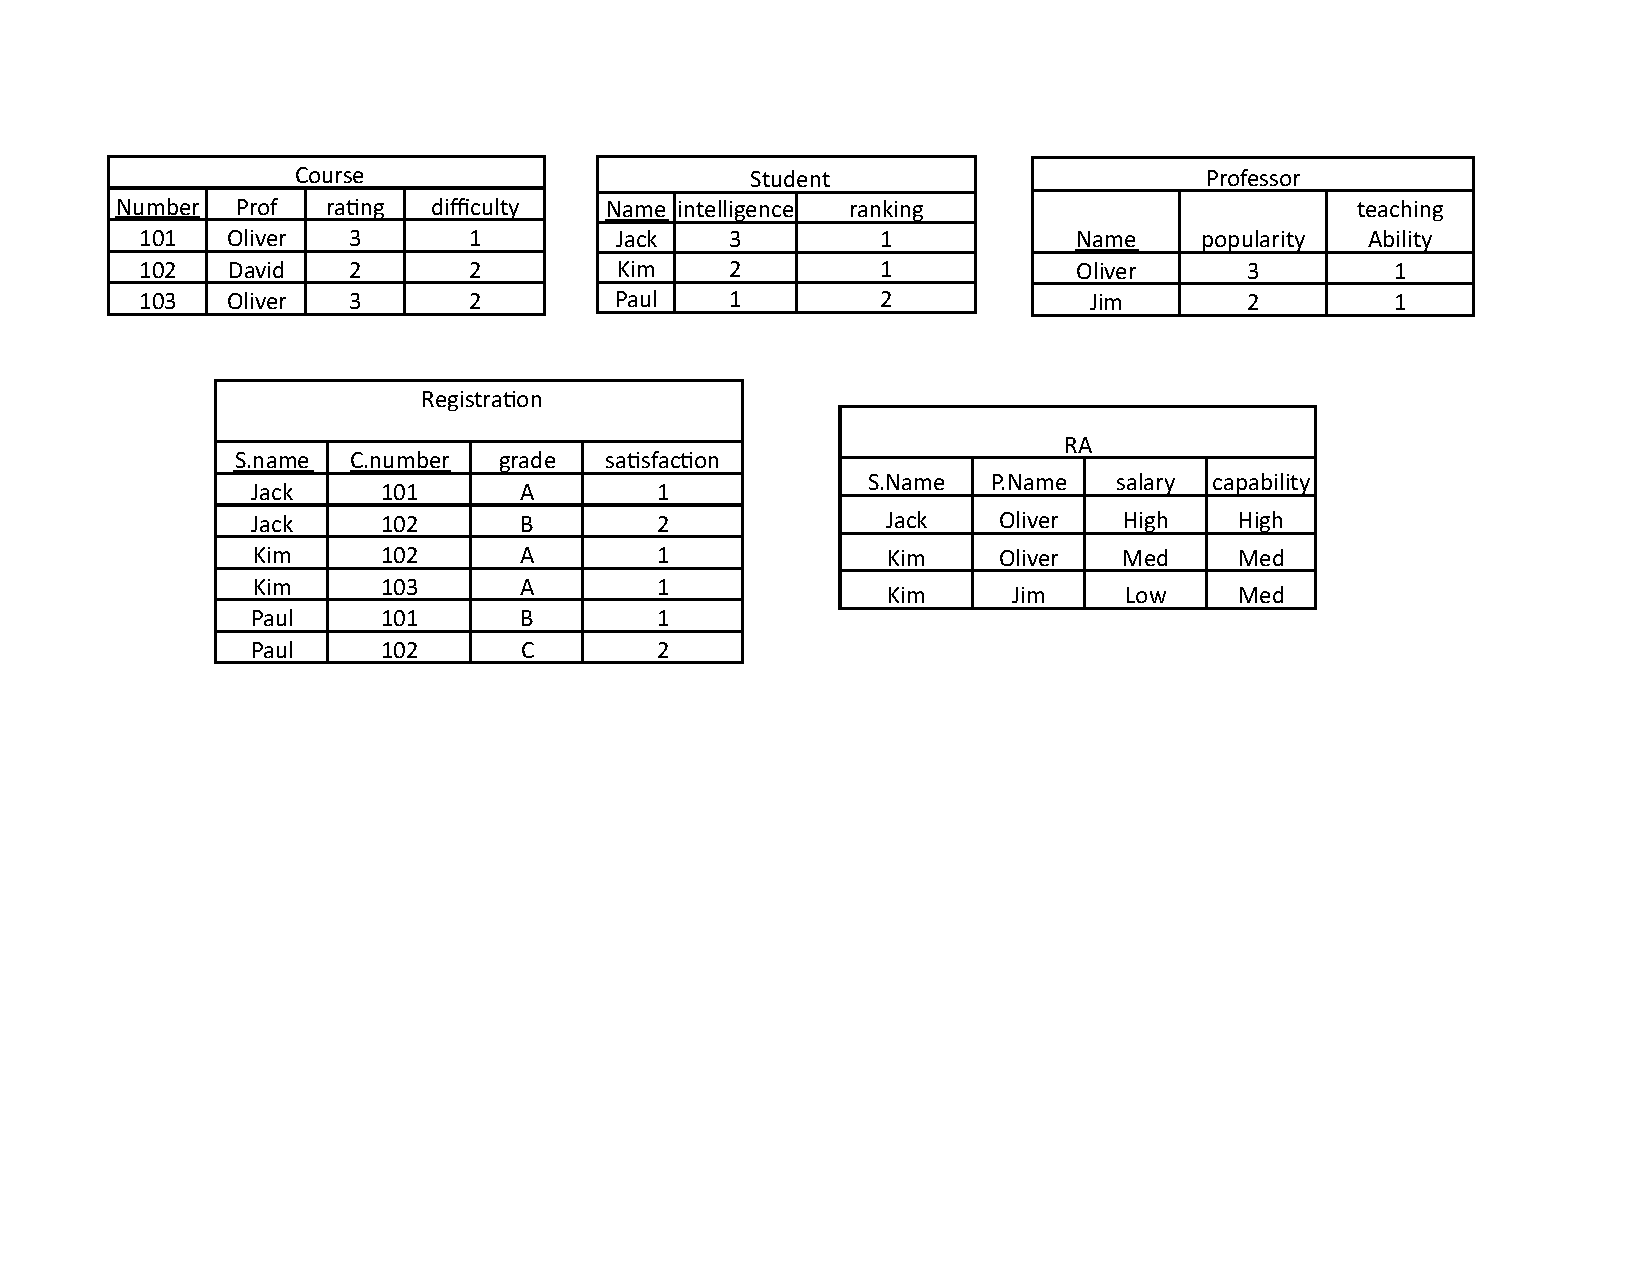
\includegraphics[width=0.7\textwidth]{db}
}
\caption{A simple relational database instance.\label{fig:db-tables}}
\end{center}
\end{figure}




\begin{figure}[htbp]
\begin{center}
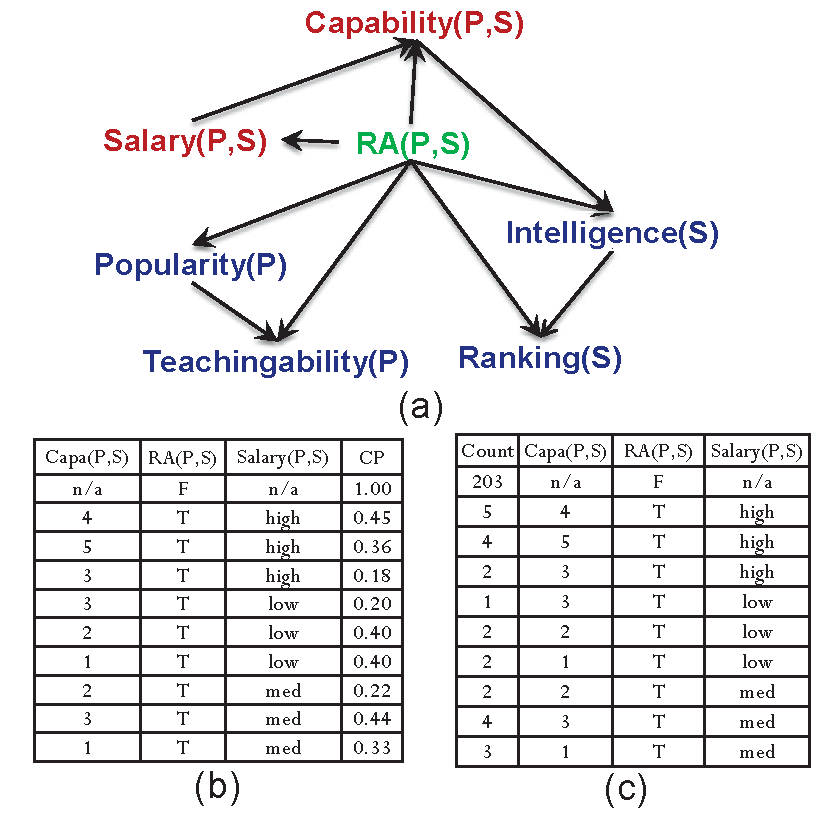
\includegraphics[width=0.7\textwidth]{pbn}
\caption{A Functor Bayes Net and its grounding for the database of Figure~\ref{fig:db-tables}. The double arrow $\leftrightarrow$ is equivalent to two directed edges. Conditional probability parameters are chosen arbitrarily for illustration.}
\label{fig:pbn}
\end{center}
\end{figure}

\begin{figure}[htbp]
\begin{center}
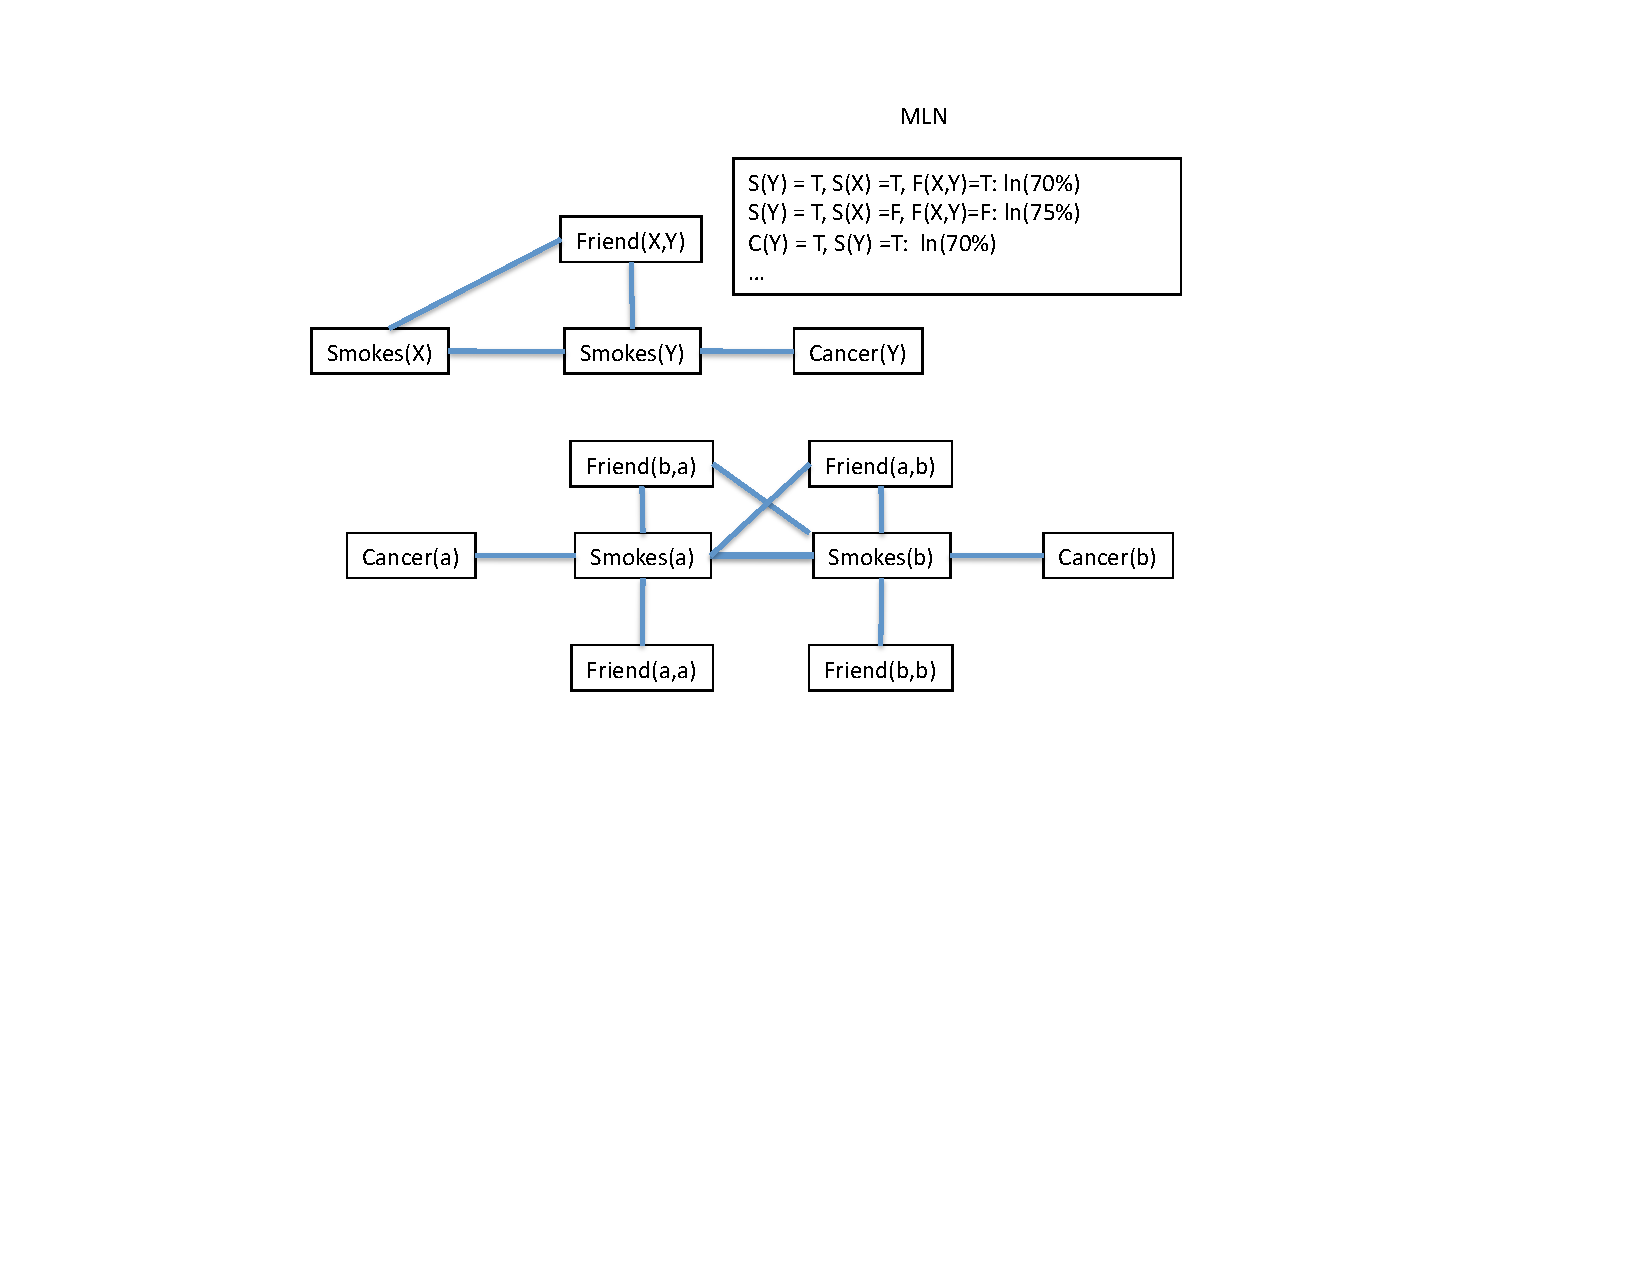
\includegraphics[width=0.7\textwidth]{mln}
\caption{The moralized Functor Bayes net of Figure~\ref{fig:pbn} and its ground Markov network for the database of Figure~\ref{fig:db-tables}. The clauses are the family formulas in the Functor Bayes net. Each clause weight is  the logarithm of the conditional probability that corresponds to the clause.}
\label{fig:mln}
\end{center}
\end{figure}


\paragraph{University Database.}
 Table~\ref{table:university-schema} shows a university relational schema and Figure~\ref{fig:university-tables} a parametrized Bayes net for this schema.

 \begin{table}[tbp] \centering
%{\small
 \resizebox{0.7\textwidth}{!}{
\begin{tabular}
[c]{|l|}\hline
$\student$(\underline{$student\_id$}, $\intelligence$, $ranking$)\\
$\it{Course}$(\underline{$\it{course}\_id$}, $\diff$, $rating$)\\
$\prof$ (\underline{$professor\_id$}, $teaching\_ability$, $popularity$)\\
$\reg$ (\underline{$student\_id$, $\it{course}\_id$}, $grade$, $satisfaction$)\\
$\it{Teaches}(\underline{\it{professor\_id, course\_id}})$
\\
\hline
$\it{RA}$ (\underline{$student\_id$, $prof\_id$}, $salary$, $capability$)\\
$\it{TA}$ (\underline{$course\_id$, $student\_id$}, $capability$)\\
\hline
\end{tabular}
}
\caption{A relational schema for a university domain. Key fields are underlined. The RA and TA relations are not used in all examples.
%An instance for this schema is given in Figure \ref{fig:university-tables}
\label{table:university-schema}}
\end{table}


%
\begin{figure}[htbp] %  figure placement: here, top, bottom, or page
   \centering
  \resizebox{0.7\textwidth}{!}{
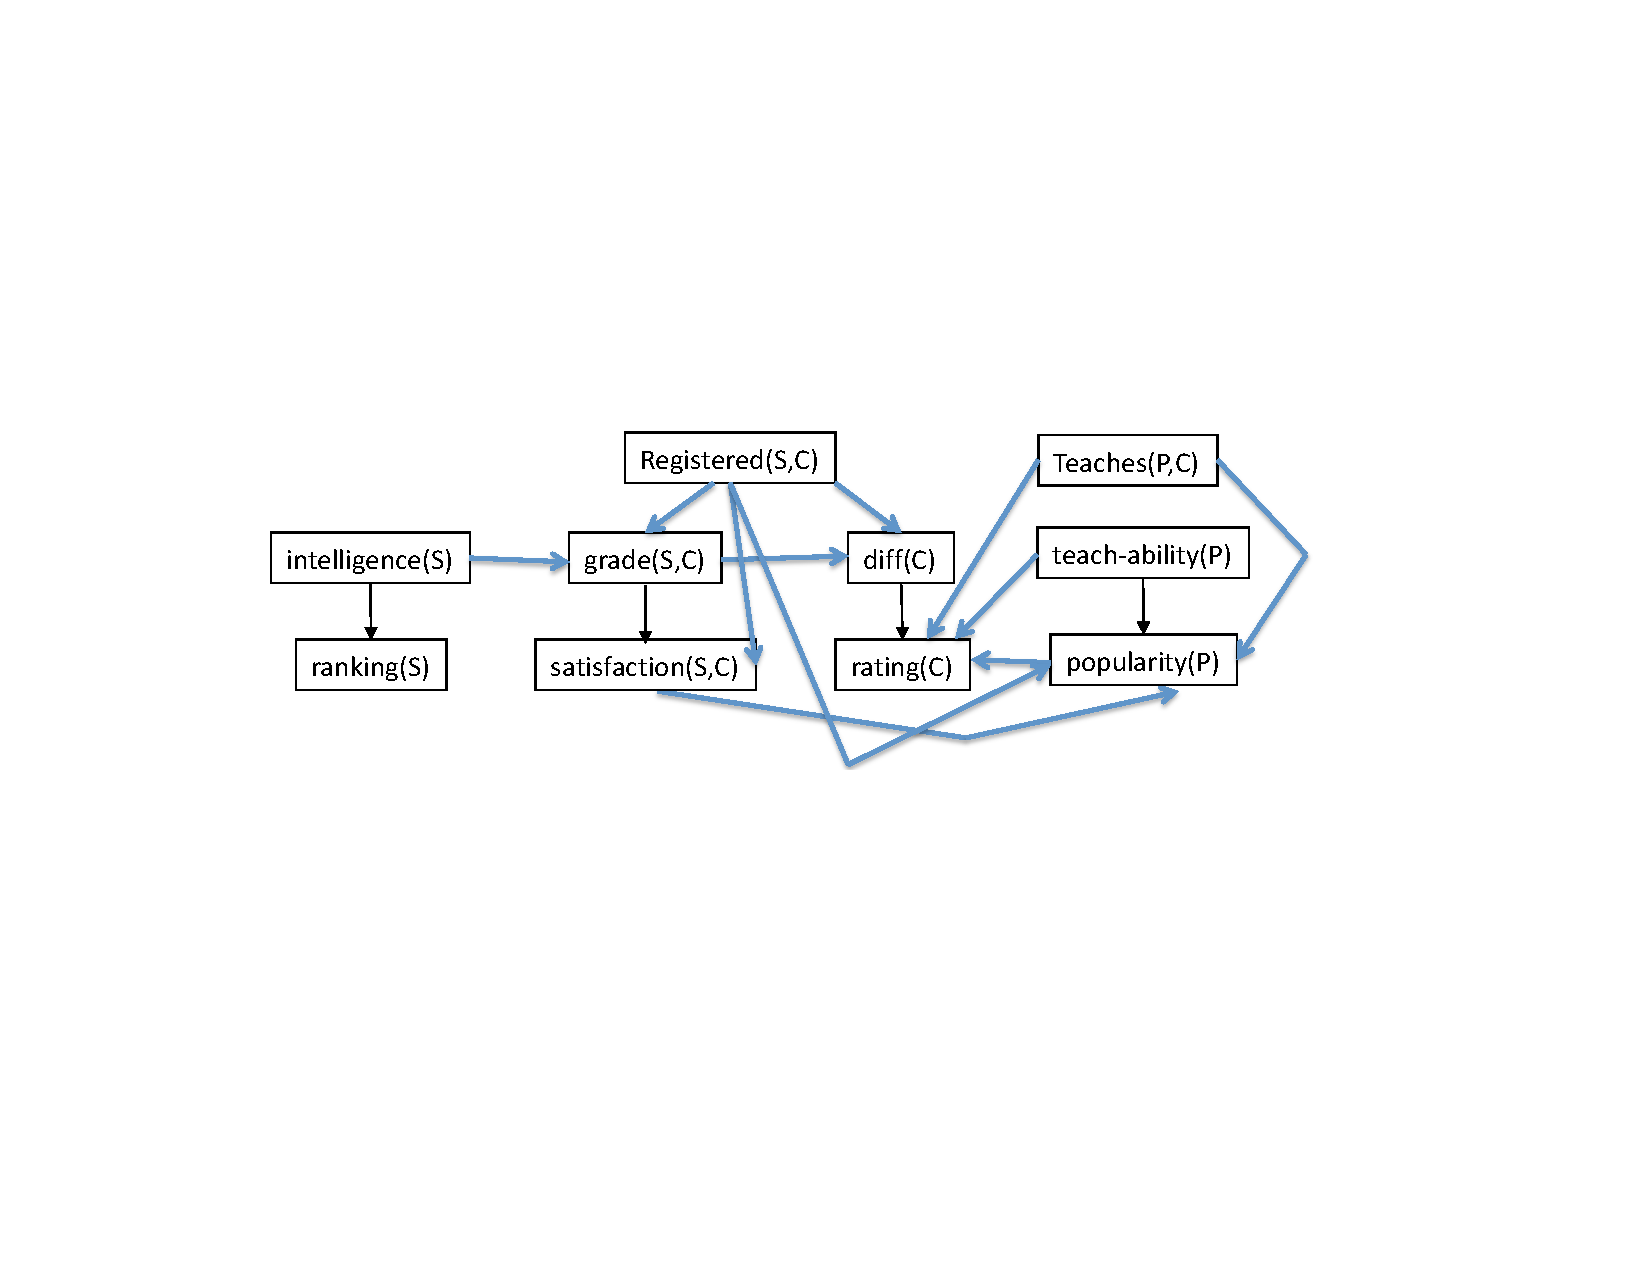
\includegraphics[width=0.7\textwidth]{uni-fbn}
}
   \caption{A Functor Bayes net graph for the relational schema of Table~\ref{table:university-schema} (without TA and RA relations). \label{fig:university-tables}}
\end{figure}

\subsection{Directed Models and the Cyclicity Problem}

In statistical-relational learning, the usual approach to inference for relational data is to use the ground graphical model for defining a joint distribution over the attributes and links of entities. This approach is known as {\em knowledge-based model construction} \cite{Ngo1997,Koller1997a,Wellman1992}. It raises two key issues.

(1) The directed model with population variables represents generic statistical relationships found in the database.
%In the terminology of Halpern \cite{Halpern90} and Bacchus \cite{Bacchus90}, the model represents type 1 probabilities or domain frequencies.
For instance, a Bayes net may encode the probability that a student is highly intelligent given the properties of a single course they haven taken. But the database may contain information about many courses that the student has taken, which needs to be combined; we may refer to this as the {\em combining problem}. In terms of the ground graph, the problem is how to define the conditional probability of a child gnode given its set of parents. For example, in the Bayes Net of Figure~\ref{fig:pbn}, the gnode $\it{Smokes}(a)$ will have a separate parent $\it{Smokes}(y)$ for each person $y$ instantiating the population variable $\Y$. (Since our toy database contains only two people, there is only one parent gnode $\it{Smokes}(b)$.) To address the combining problem, one needs to use an aggregate function, as in PRMs, or a combining rule as in BLPs, or the log-linear formula of MLNs. 

(2) Directed statistical-relational learning models face the {\em cyclicity problem}: there may be cyclic dependencies between the properties of individual entities. For example, if there is generally a correlation between the smoking habits of friends, then we may have a situation where the smoking of Jane predicts the smoking of Jack, which predicts the smoking of Cecile, which predicts the smoking of Jane, where Jack, Jane, and Cecile are all friends with each other. In the presence of such cycles, neither aggregate functions nor combining rules lead to well-defined probabilistic predictions. Figure~\ref{fig:pbn} shows a cycle of length 1 between the two gnodes $\it{Smokes}(a)$ and $\it{Smokes}(b)$. This model also illustrates how cycles arise in the presence of relationships that relate entities of the same type, as $\it{Friend}$ relates two people. Such relationships are called rings in Entity-Relationship models \cite{Ullman1982} and are called \textbf{self-relationships} by Heckerman, Koller, Meek \cite{Heckerman+al:SRL07}. Self-relationships typically give rise to \textbf{autocorrelations} where the value of an attribute for an entity depends on the value of the same attribute among related entities. For instance, in the ground Bayes net of Figure~\ref{fig:pbn}, the value of $\it{Smokes}(a)$ depends on the value of $\it{Smokes}$ for other people. 

Because cycles are not allowed in a valid Bayes net graph, grounding Functor Bayes nets that include self-relationships does not lead to a valid distribution for carrying out probabilistic inference. We refer to this as the {\em cyclicity problem}. The cyclicity problem has been difficult to solve, which has led Neville and Jensen to conclude that ``the acyclicity constraints of directed models severely limit their applicability to relational data" \cite[p.241]{bib:jensen-chapter}. Several researchers advocate the use of undirected models for relational data to avoid directed cycles. Markov random fields have therefore become a leading model class for learning and inference with relational data \cite{Domingos2007,Taskar2002}. 

The approach of this paper is essentially a hybrid method that uses directed models for learning and undirected models for inference. The idea is to use scalable Bayes net algorithms to learn a Parametrized Bayes net, then convert the Bayes net to a Markov Logic network for inference using moralization.
Converting the Bayes net to an undirected model avoids the cyclicity problem. Thus the approach of this paper combines advantages of both directed and undirected SRL models: Learning efficiency and interpretability from directed models on the one side, and on  the other, the solutions to the combining and cyclicity problems together with the inference power of undirected models.


\section{Lattice Search for Attribute Dependencies}
% Sep 27: start here.
We describe the learn-and-join method for learning a Functor Bayes net that models correlations among descriptive attributes {\em given the link structure}. We begin with the data structures that the algorithm  uses to represent relational objects. Then we give pseudocode for the algorithm and illustrate it with an example.

\subsection{Overview}

%We refer to a Functor Bayes net edge between two functors representing descriptive attributes as an Attribute-Attribute, or A2A edge.
The components of the algorithm address the following main issues.
% Pseudocode is provided as Algorithm~\ref{alg:structure}.
%The main issues are as follows.
(1) The representation of relationship sets. (2) Bounding the complexity of relational contexts. (3) Avoiding duplicate edges. (4) Propagating constraints from smaller relationship sets in the multinet lattice to larger ones.

Compared to the previous presentation of the learn-and-join algorithm by Khosravi {\em et al.} \cite{Khosravi2010}, we make two main changes. (i) We define and discuss the constraints on the graph structure that are used in the algorithm, separately from the description of the model search procedure. We also introduce some new constraints to avoid various potential redundancies. (ii) We describe the model search procedure as a lattice search, where the lattice points are chains of relationships. Conceptually, the lattice view makes the description simpler and more general without losing rigor. Computationally, the lattice diagram facilitates the implementation of the model search.

\subsection{The Multinet Lattice}
With each point in the relationship lattice, we associate a Bayes net model and a join data table. Thus the lattice structure defines a {\em multinet} rather than a single Bayes net. Multinets are a classic Bayes net formalism for modelling context-sensitive dependencies among variables. They have been applied  for modelling diverse domains, such as sleep disorders, eye diseases, and turbines that generate electricity. 
Geiger and Heckerman contributed a standard reference article for the multinet formalism  \cite{Geiger1996}.  In their illustrative example, a building guard watches for three different types of people, visitors, spies, and workers. The existence of a dependency between the gender of a person and whether or not they wear an identification badge depends on the type of person. This scenario is modelled with three multinets, one for each type of person. The type of person is the context for the corresponding multinet.

In the learn-and-join algorithm, the context of a multinet is defined by a chain of relationship functor nodes. Distinguishing these different contexts allows us to  represent that the existence of certain dependencies among attributes of entities depend on which kind of links exist between the entities. The final output of the learn-and-join algorithm is a single Bayes net derived from the multinets.

\subsubsection{The Functor Nodes} \label{sec:fnodes}
Throughout the discussion we assume that a set of functor random variables $\F$ is fixed. The random variables $\F$ are partitioned into (i) functor nodes representing descriptive attributes of entities, (ii) functor nodes representing descriptive attributes of links, (iii) Boolean relationship functor nodes that indicate whether a relationship holds. Descriptive attribute functor nodes (i) take as arguments a single population variable, whereas the relational functor nodes (ii) and (iii) take as arguments two or more population variables. %Throughout the paper w
We make the following assumptions about the functor nodes $\F$ that appear in a Functor Bayes net.

\begin{enumerate}
\item A functor node contains variables only.
\item No functor node contains the same variable $\X$ twice.
%\item Binary relationships: functors have at most two arguments.
\end{enumerate}

These assumptions are met in typical SRL models. They do not actually involve a loss of modelling power because a functor node with a constant or a repeated variable can be rewritten using a new functor symbol (provided the functor node contains at least one variable). For instance, a functor node $\it{Friend}(\X,\it{jack})$ can be replaced by introducing a new unary functor symbol $\it{Friend}_{\it{jack}}(\X)$. %(with corresponding data table) $\it{Friend}_{\it{jack}}(\X)$.
Similarly, $\it{Friend}(\X,\X)$ can be replaced by the unary functor symbol $\it{Friend}_{\it{self}}(\X)$.

The functor node set $\F$ may be explicitly specified by the user or automaticallly generated from a relational database schema \cite{Khosravi2010}.
%A simple way to generate  a default set of functor nodes is to specify a small number of population variables per entity type, say $b = 3$, so we may have variables $\X_{1},\X_{2},\X_{3}$. Then for each unary functor $\functor$, there are at most 3 functor nodes $\functor(\X_{1}),\functor(\X_{2}),\functor(\X_{3})$, and at most 6 functor nodes for binary function symbols (containing two distinct variables), such as $\functor(\X_{1},\X_{2}),\functor(\X_{1},\X_{3}),\ldots$.
%Since the functors are specified by the database schema, the bound $b$ translates a default set of functor nodes $\F$.
%Unless otherwise stated, our experiments used this default set of functor nodes with $b=3$.

{\em Examples.} The nodes of the Bayes net of Figure~\ref{fig:university-tables} are the functor nodes generated from the DB schema of Table~\ref{table:university-schema} with one population variable per entity type (e.g., $\S$ for $\it{Student}$). Self-relationships require two population variables of the same kind. This is illustrated in the Bayes net of Figure~\ref{fig:pbn}, which contains two population variables for the Person entity type $\X$ and $\Y$ for the self-relationship $\it{Friend}$. This allows the Bayes net to represent an autocorrelation involving the $\it{Smokes}$ attribute: Given that person $\X$ is friends with person $\Y$, the smoking habits of $\X$ predict those of $\Y$. 

We also assume that the functor nodes $\F$ are ordered in some way, so that a set of functor nodes corresponds to a unique ordered list. Conceptually and mathematically it is often most convenient to work with functor nodes, whereas algorithms are more easily implemented using lists. The choice of ordering does not matter for the performance of the algorithm. A concise method to define an ordering is by a lexicographic extension of an ordering on population variables as follows.

\begin{enumerate}
\item Choose an enumeration of the functors $\functor_{1},\ldots,\functor_{m}$.
\item For each entity type $\E$, with $m$ associated population variables, choose an enumeration $\X_{1},\X_{2},\ldots,\X_{m}$ of the associated variables.

\item We write $\functor(\terms)<\functor(\terms')$ for the resulting lexicographical ordering of functor nodes; that is $\functor_{i}(\terms)<\functor_{j}(\terms')$ holds if $i<j$ or if $i=j$ and the list of population variables $\terms$ is lexicographically less than the list $\terms'$.
\end{enumerate}

For instance, suppose that in Figure~\ref{fig:pbn} we order the functors as $\it{Friend} < \it{Smokes} < \it{Cancer}$ and the People variables as $\X < \Y$. The lexicographic ordering of the functor nodes is then $\it{Friend}(\X,\Y) < \it{Smokes}(\X) < \it{Smokes}(\Y) < \it{Cancer}(\Y)$.

%\subsection{The Multinet Lattice} Each point in the lattice corresponds to a subset $\set{\Relation}$ of relationship functors. With each point $\set{\Relation}$ is associated a Join Bayes net $\B_{\set{\Relation}}$ whose nodes are attribute functors, and a join data table $\Join_{\set{\Relation}}$. . The interpretation is that the Bayes net $\B_{\set{\Relation}}$ represents correlations among attributes conditional on all relationships in $\set{\Relation}$ being true. The  join data table represents a subdatabase conditional on the relationships being true.

\subsubsection{Relationship Chains}
To computationally represent sets of relationship functors, we represent them as lists without repeating elements. Assuming an ordering of relationship functors, a \textbf{relationship set} $\set{\Relation} = \{\Relation_{1}(\terms_{1}),\ldots,\Relation_{k}(\terms_{k})\}$ translates into a \textbf{relationship list} $[\set{\Relation}]=[\Relation_{1}(\terms_{1}),\ldots,\Relation_{k}(\terms_{k})]$. For order-independent concepts we refer to sets rather than to lists.
%We write $\numvariables(\set{\Relation})$ for the number of variables that occur in the relationship set.
%We associate a table join with each relationship set $\{\Relation_{1}(\terms_{1}),\ldots,\Relation_{k}(\terms_{k})\}$ as follows.
A relationship list $[\Relation_{1}(\terms_{1}),\ldots,\Relation_{k}(\terms_{k})]$ is a \textbf{chain} if each functor $\Relation_{i+1}(\terms_{i+1})$ shares at least one variable with the preceding terms $\Relation_{1}(\terms_{1}),\ldots,\Relation_{i}(\terms_{i})$.
%\footnote{Essentially the same concept is called a slot chain in PRM modelling \cite{Getoor2007c}.}
A relationship set forms a chain if the corresponding list is a chain. All sets in the lattice are constrained to form a chain.

For instance, in the University schema of Table~\ref{table:university-schema}, a %relationship 
chain is the list \[[\it{RA}(\P,\S),\it{Registered}(\S,\C)].\] If relationship node $\it{TA}(\C,S)$ is added,
%to record which student is a TA for which course,
we may have a three-element chain \[[\it{RA}(\P,\S),\it{Registered}(\S,\C),\it{TA}(\C,S)].\] The subset relation defines a lattice on relationship sets. Figure~\ref{fig:big-lattice} illustrates the  lattice for the relationship nodes in the University schema of Figure~\ref{fig:pbn}. For reasons that we explain below, entity tables are also included in the lattice and linked to relationships that involve the entity in question. 

 \begin{figure}[h]
\begin{center}
\resizebox{0.7\textwidth}{!}{
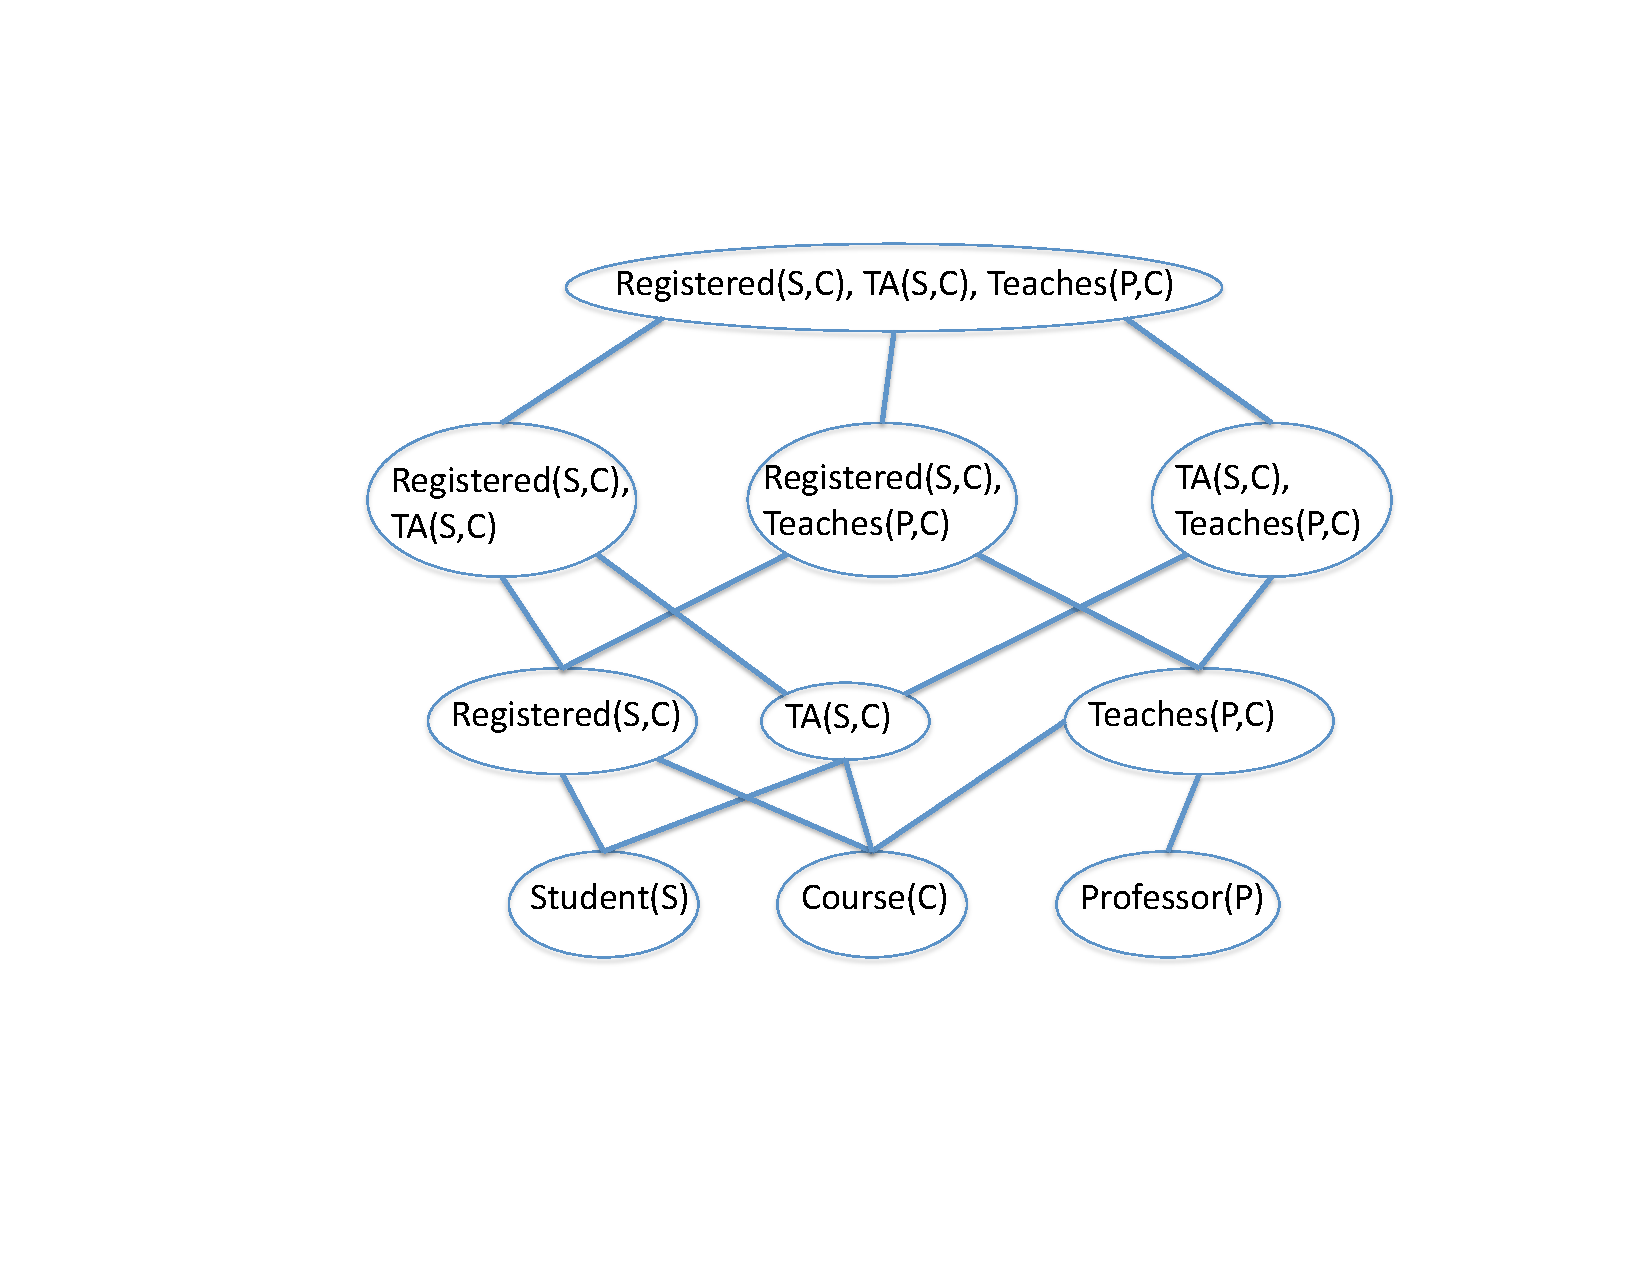
\includegraphics[width=0.7\textwidth]{big-lattice}
}
\caption{A lattice of relationship sets for the University schema of Table~\ref{table:university-schema} (without the RA relation). Links from entity tables to relationship tables correspond to foreign key pointers. The list representation of the sets is determined by the functor ordering $\it{Registered} < \it{TA} < \it{Teaches}$. \label{fig:big-lattice}}
\end{center}
\end{figure}

The concept of a relationship is related to but different from the notion of a slot chain as used in Probabilistic Relational Models \cite{Getoor2007c}. The main difference is that a slot chain can connect entity tables as well as relationship tables. 
Thus a path from the Student table to the Registered table 
to the Course table constitutes a slot chain of length 3, but contains only a single relationship (relationship chain of length 1).
% TODO: SHOW ASSOCIATED JOIN DATA TABLES.

\subsubsection{The Join Data Table} With each relationship set $\set{\Relation}$ is associated a join data table $\Join_{\set{\Relation}}$. The table represents the frequencies (sufficient statistics) with which combinations of attribute values occur, conditional on all relationships in $\set{\Relation}$ being true.
Let $\rtable_{i}$ denote the data table associated with relationship functor $\Relation_{i}(\terms_{i})$. For relationship functors $\set{\Relation} = \{\Relation_{1}(\terms_{1}),\ldots,\Relation_{k}(\terms_{k})\}$ let $\X_{1},\ldots,\X_{l}$ be the population variables that occur in the $k$ relationship functors, and write $\etable_{j}$ for the entity data table associated with the population variable $\X_{j}$. Then the join table for the relationship set, or \textbf{relationship join}, is given by

\[
\Join_{\set{\Relation}} \equiv \Join_{i=1}^{k} \rtable_{i} \Join_{j=1}^{l} \etable_{j}.
\]

If two or more variables are associated with the same population, then the same descriptive attribute will appear at least twice in the relationship join. In this case we disambiguate the names of the descriptive attributes by adding the variable as their argument. Similarly, we add variables to disambiguate repeated occurrences of descriptive link attributes. Thus each column label in the relationship join corresponds to exactly one functor node. 
%(Columns in the relationship join that do not correspond to any node in the fixed set $\F$ are omitted from the join.)
For each relationship set $\set{\Relation} = \{\Relation_{1}(\terms_{1}),\ldots,\Relation_{k}(\terms_{k})\}$, the nodes in the associated Bayes net $\B_{\set{\Relation}}$ are the column labels in $\Join_{\set{\Relation}}$, plus Boolean relationship indicator nodes $\Relation_{1}(\terms_{1}),\ldots,\Relation_{k}(\terms_{k})$.

{\em Examples.} For the relationship chain $[\it{RA}(\P,\S),\it{Registered}(\S,\C)]$, the join data table is given by
\[\it{RA}\Join \it{Registered} \Join \it{Professor} \Join \it{Student} \Join \it{Course}.\]
The join data table associated with the relationship functor $\it{Friend}(\X,\Y)$---shown in Figure ~\ref{fig:jtable}---is given by \[
\it{Friend} \Join \it{People} \Join \it{People}.\] 
%Figure~\ref{fig:jtable} shows the corresponding data table.
%
\begin{figure}[htbp]
\begin{center}
\resizebox{0.6\textwidth}{!}{
 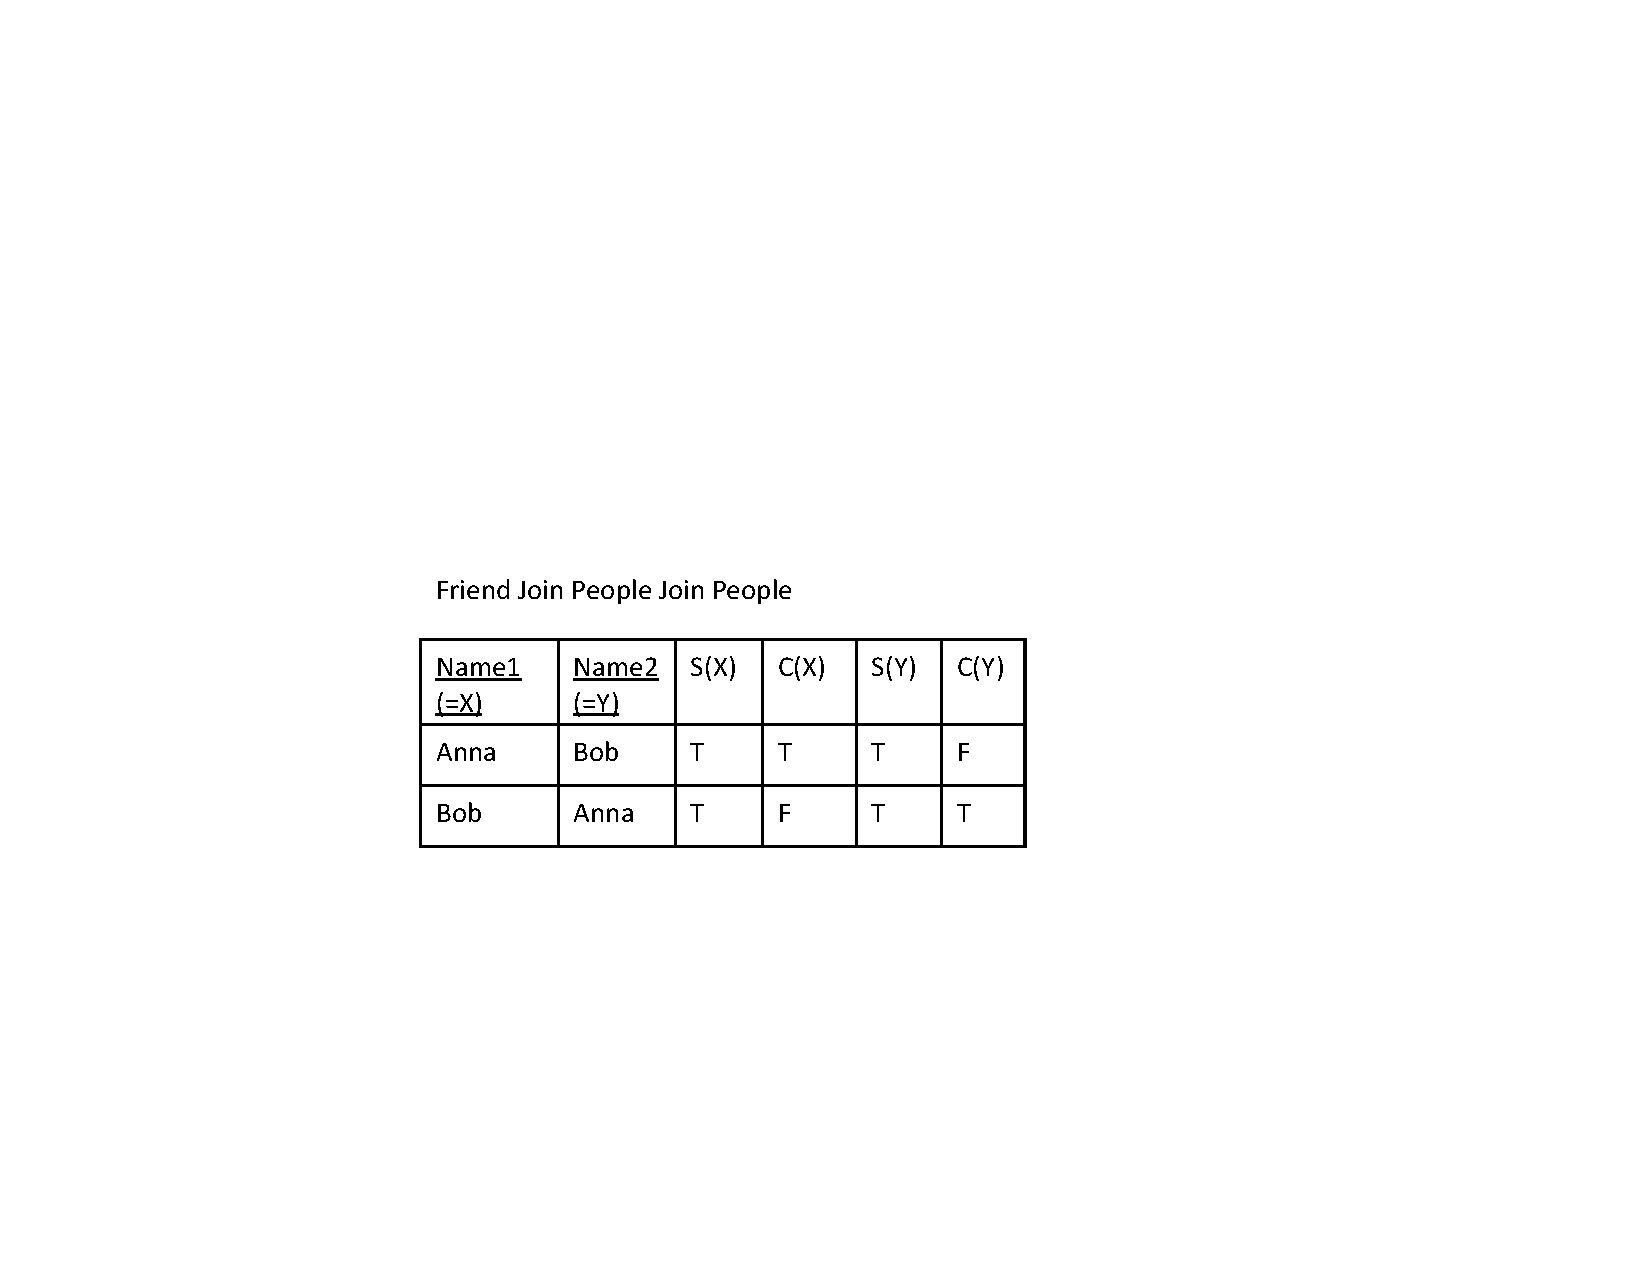
\includegraphics{jtable}
 }
\caption{The join data table associated with the $\it{Friend}$ relationship for the DB instance of Figure~\ref{fig:db-tables}.}
\label{fig:jtable}
\end{center}
\end{figure}
%
%shows the associated join data table. 

\subsection{Model Conversion} The output of the lattice search is the Bayes net associated with the largest relationship chain that forms the apex of the relationship lattice. The Bayes net of Figure~\ref{fig:university-tables} is associated with the relationship set $\it{Registered}(\S,\C),\it{Teaches}(\P,\C)$, which is the maximal conjunction of both relationship functors in this functor set. In Figure~\ref{fig:big-lattice} the maximally large relationship set has three members. For Markov Logic Networks, we convert the maximal Bayes net to an MLN using moralization. The Bayes net can similarly be converted to other clausal formalisms like BLPs and LBNs, since an  Functor Bayes net defines a set of directed clauses of the form $\it{child} \leftarrow \it{parents}$  \cite{Kersting2007}.
% and the union of these clauses over maximal Functor Bayes nets defines the complete set. 
%
% there is only one maximally large relationship set with three members. 
%A multi-net lattice can be straightforwardly converted to other SRL formalisms as follows. Say that a Functor Bayes net associated with a maximally large relationship set is maximal. 
%In Figure~\ref{fig:big-lattice} there is only one maximally large relationship set with three members. For Markov Logic Networks, the focus of this paper, we convert the maximal Functor Bayes nets to MLNs using moralization; the union of these MLNs is the final output MLN. A multi-net lattice can similarly be converted to other clausal formalisms like BLPs and LBNs: A single Functor Bayes net defines a set of directed clauses of the form $\it{child} \rightarrow \it{parents}$ and the union of these clauses over maximal Functor Bayes nets defines the complete set. The most complicated case arises if an application requires a single Functor Bayes net for the entire database, but the union of the maximal Functor Bayes net graphs is not acyclic. In this case it may be possible to apply a Bayes net combining algorithm to merge the maximal Functor Bayes nets into a single one \cite{Tillman2008}.

\section{The Learn-And-Join Algorithm} \label{Sec:LAJ}

This section presents the Learn-and-Join Algorithm (LAJ) that takes as input a relational database and constructs a Functor Bayes multinet for each relationship set in the multinet lattice.
%If an application requires a single Bayes net for the entire database, the lattice multinet can be converted to a single Bayes net by applying a Bayes net combining algorithm [Tilman].
The algorithm enumerates relationship lists. This can be done using any standard technique, such as those developed for enumerating itemsets in association rule  mining \cite{Agrawal1994}.  It proceeds level-wise by considering relationship sets of length $s = 1, 2, \ldots$. After Bayes nets have been learned for sets of length $s$, the learned edges are propagated to sets of length $s+1$. In the initial case of single relationship tables where $s=1$, the edges are propagated from Bayes nets learned for entity tables. In addition to the edge constraints, the algorithm enforces a number of constraints that are motivated by the relational structure of the functor nodes.

We next provide a compact description of the constraints used, including their definition, an intuitive interpretation and examples. Then we show by examples how the constraints operate. Finally, we summarize the algorithm with pseudocode as Algorithm~\ref{alg:structure}. Later sections discuss the constraints in detail, including motivation, mathematical analysis and references to related concepts that have appeared in the literature.

\subsection{Constraints Used in the Learn-And-Join Algorithm}

The constraints fall into two types: relational constraints that capture the semantics of the relational schema, and lattice constraints on the presence/absence of edges that connect the results of learning from different points in the relationship set lattice. 


The algorithm requires the specification of a main population variable for each entity type (e.g., $\Y$ for $\it{People}$). The intuitive interpretation is that the distribution of attributes for that entity type is modelled by functor nodes that involve the main variable, whereas other functor nodes play an auxilliary role (e.g., the distribution of the $\it{S mokes}$ attribute is modelled by the functor node $\it{Smokes}(\Y)$ rather than the functor node $\it{Smokes}(\X)$).


\subsubsection{Edge Inheritance In the Relationship Lattice}
These constraints state the presence or absence of edges in graphs associated with join tables lower in the lattice is inherited by graphs associated with join tables higher in the lattice. The intuition behind these constraints is that dependencies should be assessed in the most specific context possible. First edges from an entity table are inherited by relationship tables that involve the entity in question.

\begin{constraint} \label{clause:econstraints} Let $\X$ be the main population variable for an entity type associated with entity table $\etable$. Let $\set{\Relation}$ be any relationship set that contains the variable $\X$. Then the Bayes net associated with $\set{\Relation}$ contains an edge $\functor(\X) \rightarrow g(\X)$ connecting two descriptive attributes of $\X$ if and only if the Bayes net associated with $\etable$ contains the edge $\functor(\X) \rightarrow g(\X)$.
\end{constraint}

{\em Example.} 
If the $\it{People}$ Bayes net contains an edge $\it{Smokes}(\Y) \rightarrow \it{Cancer}(\Y)$, then the Bayes net associated with the relationship $\it{Friend}$ must also contain this edge (see Figure~\ref{fig:pbn}). If the edge is absent in the $\it{People}$ Bayes net, it must also be absent in the Bayes net associated with the relationship $\it{Friend}$.

The next constraint states that edges learned on smaller relationship sets are inherited by larger relationship sets. If the smaller sets are ambiguous with regard to the direction of an adjacency, the larger relationship set must contain the adjacency; the direction is then resolved by applying Bayes net learning to the larger relationship set.

\begin{constraint} \label{clause:rconstraints} Suppose that nodes $\functor(\terms),g(\terms')$ appear in the join table $\Join_{\set{\Relation}}$.
% and also in a subset join $\Join_{\set{\Relation'}}$ where $\set{\Relation}'$ is a subset of $\set{\Relation}$. 
Then
\begin{enumerate}
\item  If $\functor(\terms)$ and $g(\terms')$ are not adjacent in any graph $\B_{\set{\Relation}^{*}}$ associated with a relationship subset $\set{\Relation}^{*} \subset \set{\Relation}$, then $\functor(\terms)$ and $g(\terms')$ are not adjacent in the graph associated with the relationship set $\set{\Relation}$.
\item Else if all subset graphs agree on the orientation of the adjacency  $\functor(\terms)-g(\terms')$, the graph associated with the relationship set $\set{\Relation}$ inherits this orientation.
\item Else the graph associated with the relationship set $\set{\Relation}$. must contain the edge $\functor(\terms) \rightarrow g(\terms')$ or the edge $\functor(\terms) \leftarrow g(\terms')$.
\end{enumerate}
\end{constraint}

{\em Examples.} 
Consider the lattice shown in Figure~\ref{fig:big-lattice}. 
Suppose that the graph associated with the relationship $\it{Registered}(\S,\C)$ contains an edge $$\it{difficulty}(\C) \rightarrow \it{intelligence}(\S),$$ and that the graph associated with the relationship $\it{TA}(\S,\C)$ does not contain the edge $\it{difficulty}(\C) \rightarrow \it{intelligence}(\S)$. 
%(The latter will be the case since the relationship set $\it{TA}(\S,\C)$ does not contain the variable $\S$.)
% actually, the answer is that the main functor constraint overrides the inheritance constraint.
Then the edge $\it{difficulty}(\C) \rightarrow \it{intelligence}(\S)$ must be present in the Bayes net associated with the larger relationship set $\it{Registered}(\S,\C)$, $\it{TA}(\S,\C)$. If the edge is contained  in neither of the graphs associated with $\it{Registered}(\S,\C)$, and $\it{TA}(\S,\C)$, it must not be present in the graph associated with the $\it{Registered}(\S,\C)$, $\it{TA}(\S,\C)$.


\subsubsection{The Main Functor Node Format}
The algorithm requires the specification of a main functor node for each functor (e.g., $\it{Smokes}(\Y)$ is the main functor node for the functor $\it{Smokes}$). Only main functor nodes are allowed to have edges pointing into them (i.e., indegree greater than 0). The intuition behind this constraint is that it suffices to model the conditional distribution of just one ``copy'' of the functor. For example, to model the conditional distribution of the $\it{Smokes}$ attribute, it suffices to have parents only for  the functor node $\it{Smokes}(\Y)$, rather than allow parents for both the functor node $\it{Smokes}(\Y)$ and $\it{Smokes}(\X)$. One way to define main functor nodes is in terms of a lexicographic ordering derived from an ordering of population variables (cf. Section~\ref{sec:fnodes}). That is, the main node for function symbol $\functor$ is the functor $\functor(\term)$ where $\term$ is the lexicographically first list of terms for $\functor$. We refer to such Functor Bayes nets as
\textbf{main variable} Functor Bayes nets. 


\begin{constraint}
For any Bayes net associated with a relationship set, if its graph contains an edge $ \rightarrow \functor(\terms)$ pointing into a node $\functor(\terms)$, then $\functor(\terms)$ is the main functor node for $\functor$. 
% $\functor(\terms) \rightarrow g(\terms')$ then $g(\terms')$ is the main functor node for $g$. 
 \label{clause:head}
\end{constraint}

{\em Example.} Suppose that $\it{Smokes}(\Y)$ is the main functor node for $\it{Smokes}$. Then the main functor constraint permits the edges $\it{Smokes}(\X) \rightarrow \it{Smokes}(\Y)$ and $\it{Friend}(\X,\Y) \rightarrow \it{Smokes}(\Y)$, but rules out the edges $\it{Smokes}(\Y) \rightarrow \it{Smokes}(\X)$ and $\it{Friend}(\X,\Y) \rightarrow \it{Smokes}(\X)$.

%\subsubsection{Connectivity}
%
%The attributes of two distinct entities are independent of each other unless we condition on the information that there is a link between them, or a chain of links. More generally, in the database distribution two \marginpar{need to define database distribution} nodes are independent of each other unless we condition on shared links. As a graphical constraint, this means that we consider only edges between nodes that are connected by the given relationship context.
%
%\begin{constraint} \label{clause:connectivity}
%if the Bayes net associated with a relationship set $\set{\Relation}$ contains an edge $\functor(\terms) \rightarrow g(\terms')$, then both $\functor(\terms)$ and $g(\terms')$ share at least one population variable with $\set{\Relation}$.
%\end{constraint}
%
%{\em Example.} In the graph associated with the relationship set $\it{Registered}(\S,\C)$, 
%
%[Comment: this seems to be redundant because of the way nodes are associated with a relationship set].

 
\subsubsection{Population Variable Bound}
We allow the user to specify a bound on the number of population variables that occur in a family (child + parent nodes). Intuitively, this bounds the number of distinct (generic) objects that can be considered in a single child-parent configuration. For instance, if the bound is 1, the family expresses patterns only about a single entity. With 2 population variables, patterns involving pairs can be expressed, with 3 triples can be modelled, etc. 

{\em Examples.} For the node $\it{Cancer}(\Y)$ of Figure~\ref{fig:pbn}, its family contains a single population variable $\Y$, so only patterns involving a generic person can be represented. For the node $\it{Smokes}(\Y)$, its family  contains two population variables $\X$ and $\Y$, so patterns involving pairs of people can be represented.

We emphasize that a variable number bound does not imply any bound on the length of clauses: even with a single population variable like $\S$ associated with students, we can have an arbitrary number of attributes of students in a single clause. Kok and Domingos \cite{Kok2010} highlight the importance of learning long clauses for relational models. 


\subsubsection{Link Attributes} There is a deterministic dependency between a Boolean relationship indicator node  and a descriptive attribute associated with the relationship: If the relationship does not exist between two entities, then the value of the descriptive attribute is undefined. In our representation, this means that the descriptive attribute takes on the value $\bot$ for undefined (cf. Section~\ref{sec:functors}). This deterministic connection can be enforced given the following graphical constraint. 

\begin{constraint} \label{clause:r2ra} Suppose that $\functor_{\Relation}$ denotes a descriptive attribute of relationship $\Relation$ and that $\f_{\Relation}(\terms)$ is the main functor node for $\f_{\Relation}$ and $\Relation(\terms)$ is the main functor node for $\Relation$. Then there is an edge 

$\Relation(\terms) \rightarrow \f_{\Relation}(\terms)$ in any Bayes net that contains $\f_{\Relation}(\terms)$.
\end{constraint}

{\em Examples.} In the Bayes net of Figure~\ref{fig:university-tables}, the functors $\it{satisfaction}$ and $\it{grade}$ denote descriptive attributes of the $\it{Registered}$ relationship. So the Bayes net must contain edges $\it{Registered}(\S,\C) \rightarrow \it{satisfaction}(\S,\C)$ and $\it{Registered}(\S,\C) \rightarrow \it{grade}(\S,\C)$, which are the main nodes for their respective functors.

%Clause~\ref{clause:r2ra} models the deterministic impact of a relationship indicator variable $\Relation(\term)$ on each descriptive attribute $\functor_{\Relation}(\term)$ of the relationship: if $\Relation(\term) = \false$, then with probability 1, $\functor_{\Relation}(\term) = \bot$. Clause~\ref{clause:rcontext} says that if an association between attributes $\functor(\terms) \rightarrow g(\terms')$ depends on the relational context $\set{\Relation}$, then the Bayes net must include the relationship functors in $\set{\Relation}$ as parents of $g(\terms')$ in order to indicate the context-dependence. 
We discuss and analyze
%these and the other 
the constraints further in later sections.
%in the following sections. 
The next subsection presents examples of how the constraints operate in the learn-and-join algorithm.

%
%\begin{table}[htpb] \caption{Constraints for lattice multinets that represent dependencies among descriptive attributes. The notation $\B_{\etable}$  denotes the Bayes net associated with entity table $\etable$, the notation $\B_{\set{\Relation}}$ the Bayes net associated with relationship set $\set{\Relation}$.\label{table:a2a}}
%\begin{enumerate}
%\item Forbidden Edges I: if $\B$ contains $\functor(\terms) \rightarrow g(\terms')$ then $g(\terms')$ is the main functor for attribute $g$. \label{clause:head}
%\item Forbidden Edges II: if $\B_{\set{\Relation}}$ contains $\functor(\terms) \rightarrow g(\terms')$, then both $\functor(\terms)$ and $g(\terms')$ share at least one population variable with $\set{\Relation}$.
%\item Required Edges: $\Relation(\terms) \rightarrow \f_{\Relation}(\terms)$ where $\functor_{\Relation}$ is a descriptive attribute of relationship $\Relation$ whose main node is $\f_{\Relation}(\terms)$. \label{clause:r2ra}
%\item Lattice Constraints I: Suppose that (i) unary main nodes $\functor(\X)$ and $g(\X)$ appear in the join associated with relationship set $\set{\Relation}$, and (ii) $\X$ is the main population variable for the entity table $\etable$. % be the entity table for population variable $\X$.
%  Then there is an edge $\functor(\X) \rightarrow g(\X)$ in $\B_{\set{\Relation}}$ if and only if there is the same edge $\functor(\X) \rightarrow g(\X)$ in $\B_{\etable}$.\label{clause:econstraints}
%\item \label{clause:rconstraints} Lattice Constraints II: Suppose that nodes $\functor(\terms),g(\terms')$ appear in the join table $\Join_{\set{\Relation}}$ and also in a subset join $\Join_{\set{\Relation'}}$ with $\set{\Relation}' \subset \set{\Relation}$. Then
%\begin{enumerate}
%\item  If $\functor(\terms)$ and $g(\terms')$ are not adjacent in any subset graph $\B_{\set{\Relation}^{*}}$ with $\set{\Relation}^{*} \subset \set{\Relation}$, then $\functor(\terms)$ and $g(\terms')$ are not adjacent in the graph $\B_{\set{\Relation}}$.% associated with the relationship set $\set{\Relation}$.
%\item Else if all subset graphs agree on the orientation of the adjacency  $\functor(\terms)-g(\terms')$, the graph $\B_{\set{\Relation}}$ inherits this orientation.
%\item Else the graph $\B_{\set{\Relation}}$ must contain the edge $\functor(\terms) \rightarrow g(\terms')$ or the edge $\functor(\terms) \leftarrow g(\terms')$.
%\end{enumerate}
%\item \label{clause:rcontext} Lattice Constraints III: If the edge $\functor(\terms) \rightarrow g(\terms')$ appears in a graph $\B_{\set{\Relation}}$ but not in any graph associated with a subset of $\set{\Relation}$, then add edges $\Relation(\terms^{*}) \rightarrow g(\terms')$ for each relationship indicator node $\Relation(\terms^{*}) \in \set{\Relation}$.
%\end{enumerate}
%\end{table}


\subsection{Examples.} We illustrate the learn-and-join algorithm on the example database of Figure~\ref{fig:db-tables}; see Figure~\ref{fig:friend-mnl}. The $\it{TA}$ and $\it{RA}$ relations are omitted for simplicity.

\begin{enumerate}
\item Applying the single-table Bayes net learner to the $\it{People}$ table may produce a single-edge graph $\it{Smokes}(\Y) \rightarrow \it{Cancer}(\Y)$.
\item Then form the join data table \[\jtable = \it{Friend} \Join \it{People} \Join \it{People}\] shown in Figure~\ref{fig:jtable}.
The Bayes net learner is applied to $\jtable$, with the following constraints.
\begin{enumerate}
\item From the $\it{People}$ Bayes net, there must be an edge $\it{Smokes}(\Y) \rightarrow \it{Cancer}(\Y)$, where $\Y$ is the main population variable associated with $\it{People}$. (Constraint(\ref{clause:econstraints})).
\item No edges may point into $\it{Smokes}(\X)$ or $\it{Cancer}(\X)$, since these are not the main functor nodes for the functors $\it{Smokes}$ and $\it{Cancer}$. 
%$\X$ is not the main variable for $\it{People}$ 
(Constraint~\ref{clause:head}). 
\end{enumerate}
\end{enumerate}
The Bayes net learner applied to the join table $\jtable$ then may find an edge $\it{Smokes}(\X) \rightarrow \it{Smokes}(\Y)Lattice Constraints from relationship joins of size$. Since the dependency represented by this edge is valid only for pairs of people that are friends (i.e., conditional on $\it{Friend}(\X,\Y) = \true$), the algorithm adds an edge $\it{Friend}(\X,\Y) \rightarrow \it{Smokes}(\Y)$ %(Constraint(\ref{clause:rcontext})),
whose associated Bayes net is shown in Figure~\ref{fig:friend-mnl}. 

Figure~\ref{fig:uni-tables} shows the multinet for the University schema up to level 1. Continuing the construction up to the highest level 2 produces a single Bayes net for the maximal relationship set $\it{Registered}(\S,\C),\it{Teaches}(\P,\C)$ that is shown in Figure~\ref{fig:university-tables}.

\begin{figure}[htbp]
\begin{center}
  \resizebox{0.7\textwidth}{!}{
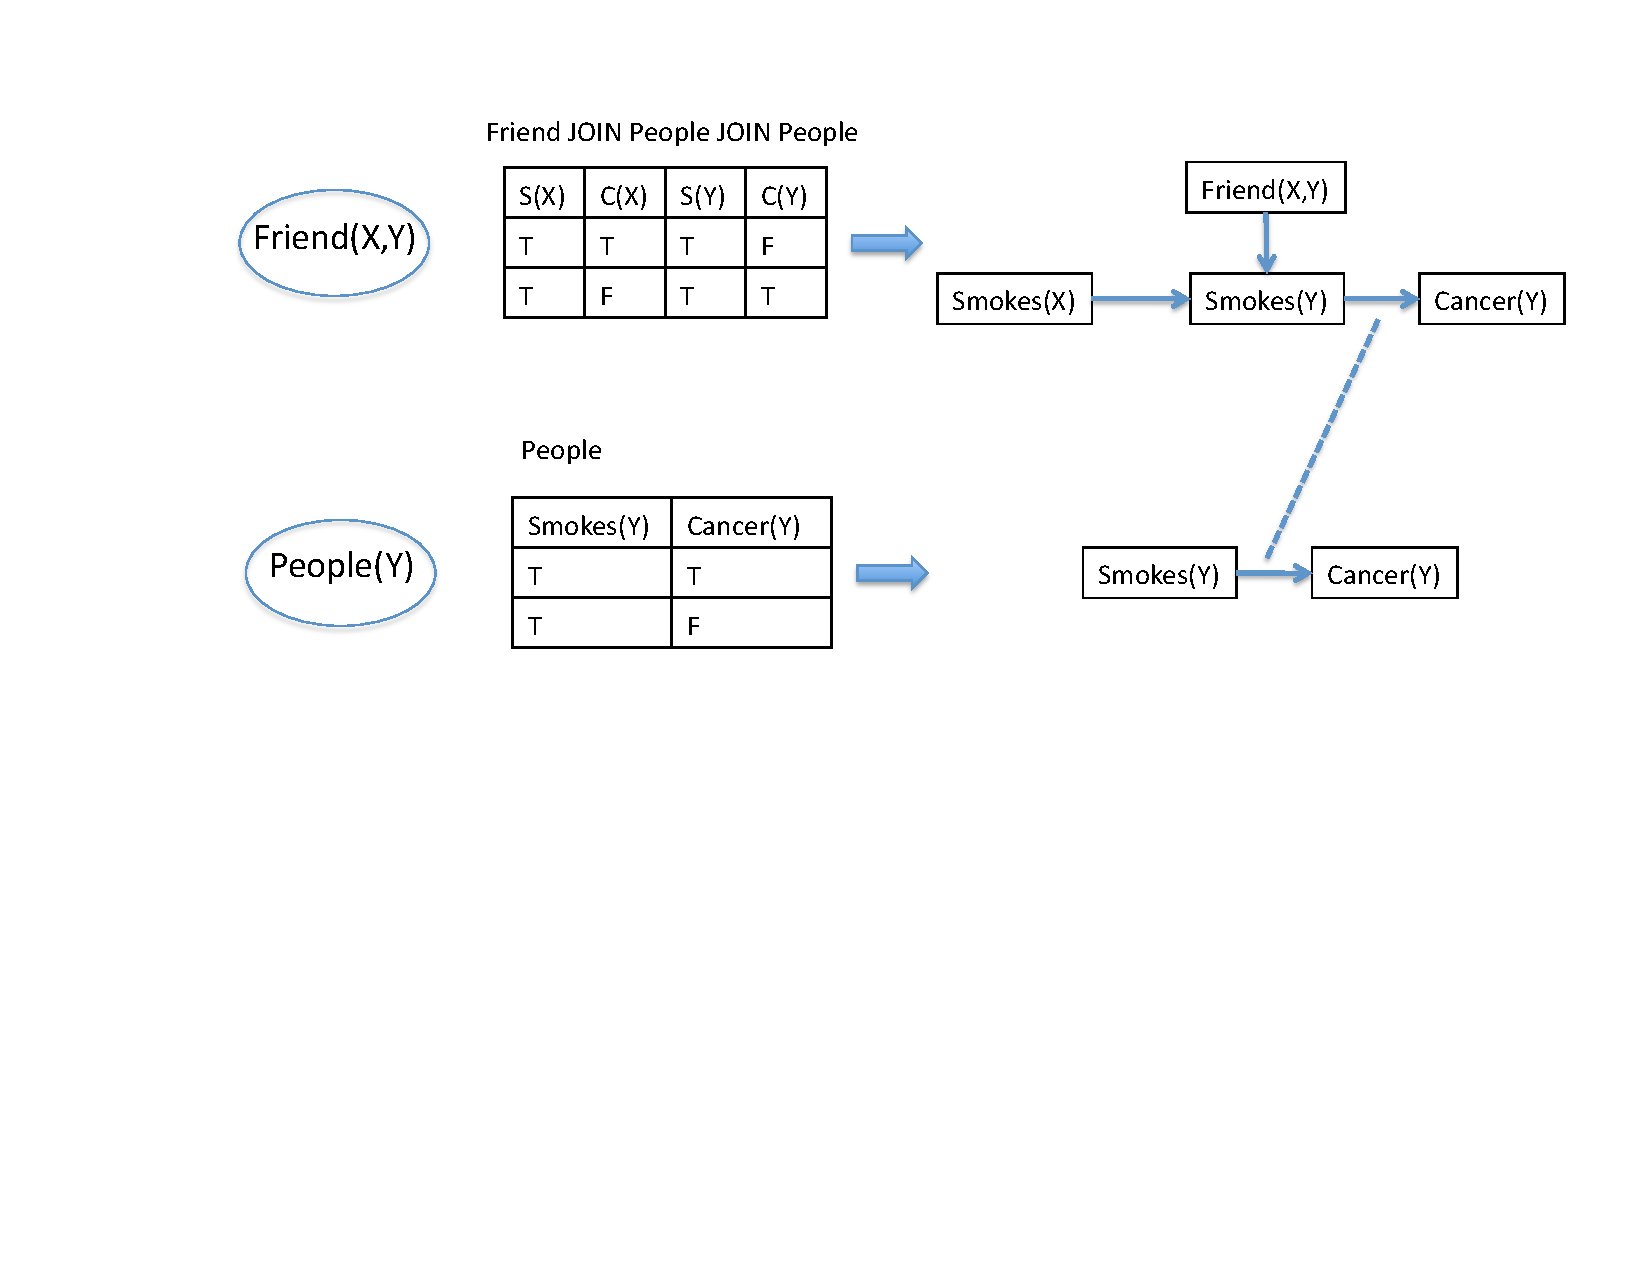
\includegraphics{friend-mn}
}\caption{The 2-net lattice associated with the DB instance of Figure~\ref{fig:db-tables}. The figure shows the data tables associated with the only entity table $\it{People}$ and the only relationship table $\it{Friend}$. The block arrow indicates that the output of a single-table Bayes net learner on the data table is the Bayes net shown. The dashed line that connects the two edges $\it{Smokes}(\Y) \rightarrow \it{Cancer}(\Y)$ indicates that this  edge is propagated from the lower-level Bayes net to the higher-level Bayes net.}
\label{fig:friend-mnl}
\end{center}
\end{figure}

  \begin{figure}[h]
\begin{center}
\resizebox{0.7\textwidth}{!}{
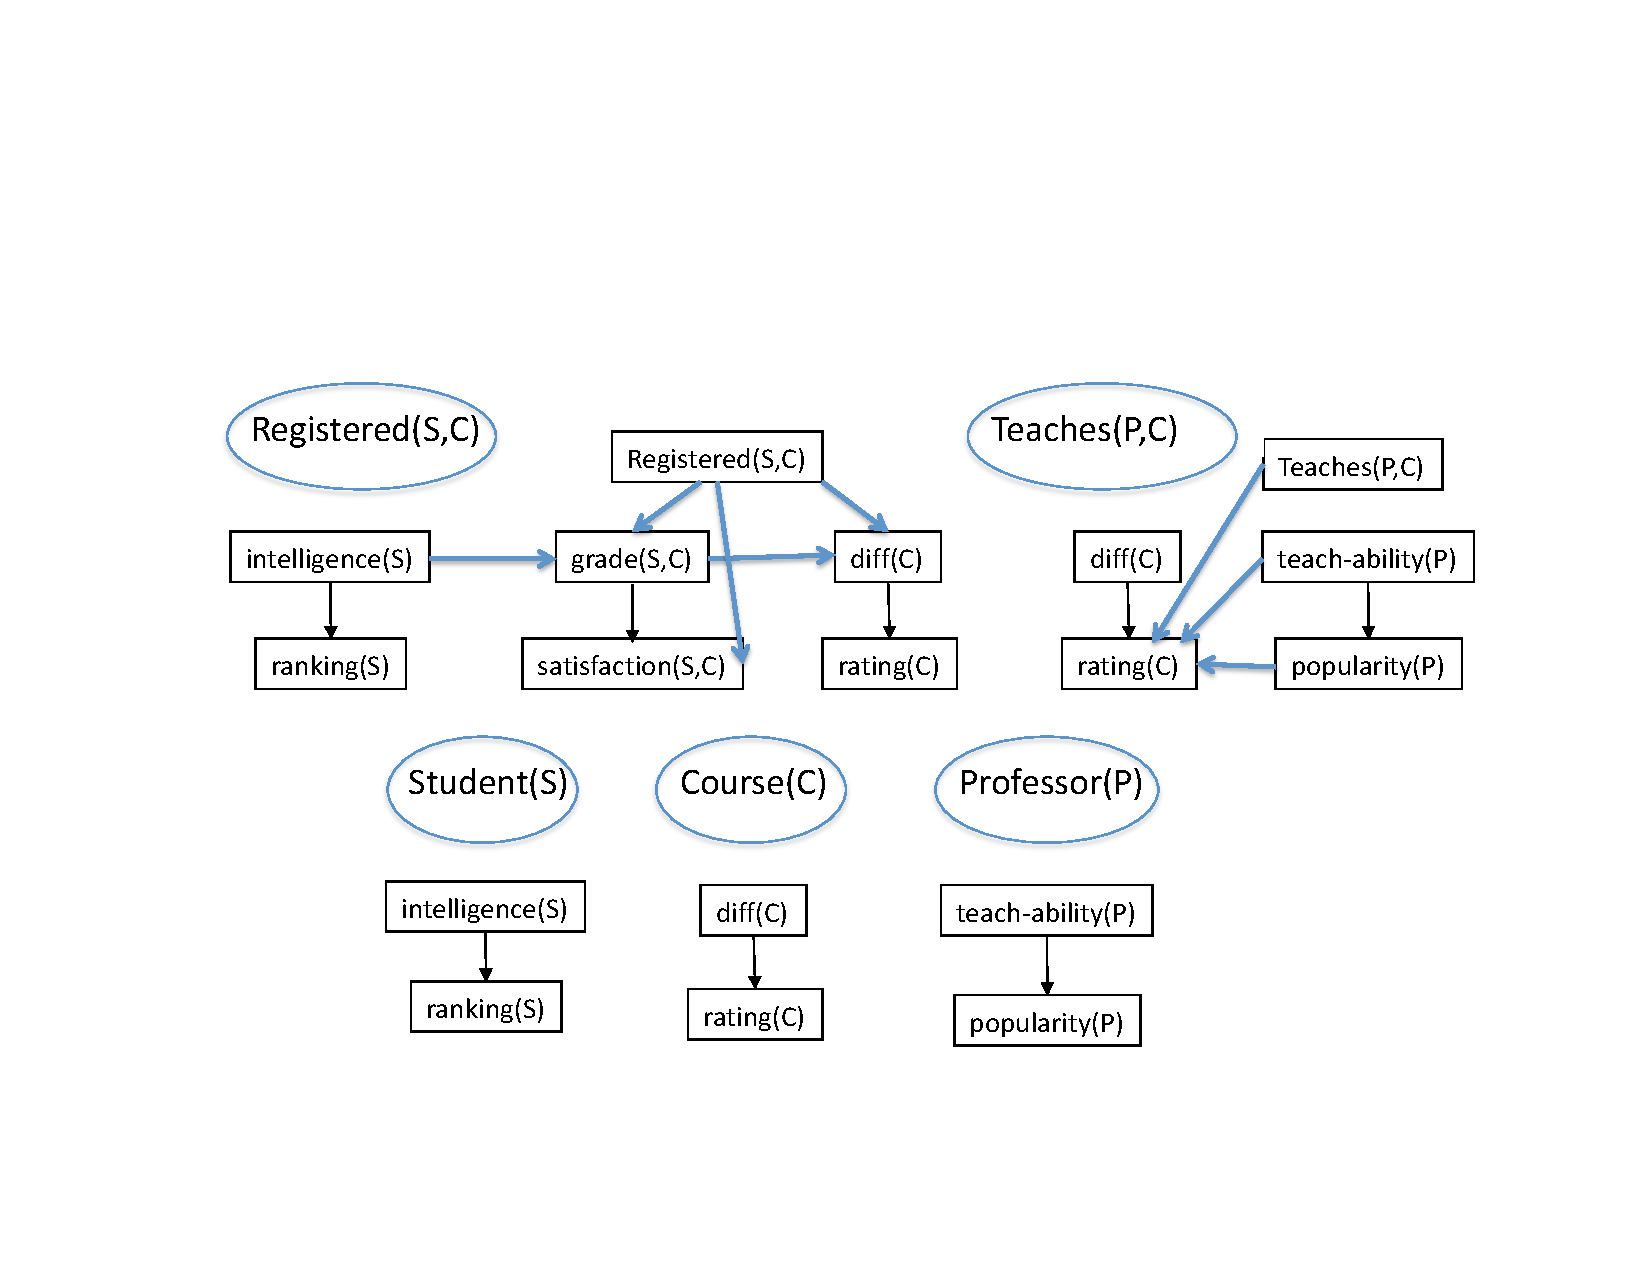
\includegraphics[width=0.7\textwidth]{uni-tables}
}
\caption{The multinet lattice for the University Schema, restricted to %single 
entity and relationship functors. Join data tables are not shown. We omit the $\it{TA}$ and $\it{RA}$ relationships for simplicity.\label{fig:uni-tables}}
\end{center}
\end{figure}
%
%  \begin{figure}[h]
%\begin{center}
%\resizebox{0.7\textwidth}{!}{
%\includegraphics[width=0.7\textwidth]{uni-bignet}
%}
%\caption{The multinet lattice for the University Schema (ii): for the maximal relationship set $\it{Registered}(\S,\C),\it{Teaches}(\P,\C)$. The join data table is not shown. We omit the $\it{TA}$ relationship for simplicity. \label{fig:uni-bignet}}
%\end{center}
%\end{figure}

\subsection{Pseudocode}

Algorithm~\ref{alg:structure} combines all the algorithm's components in pseudocode. We next discuss the constraints in more detail, including a mathematical analysis of the most important ones.

\begin{algorithm}[htbp]
%\linesnumbered
\SetKwData{Calls}{Calls}
\SetKwData{Notation}{Notation}
%\begin{algorithmic}
%{\footnotesize
%\STATE {\em Input}: Database $\D$ with $\etable_1,..\etable_e$ entity tables, functors $\F$, variable number bound $\varbound$.
\KwIn{Database $\D$ with  entity tables $\etable_1,..\etable_e$; functors $\F$; \#variable bound $\varbound$.}
\KwOut{MLN formulas for $\D$; a Bayes multi-net $\B_{\set{\Relation}}$ for relationship subsets of $\F$.}
\begin{algorithmic}
\STATE \Calls BNL: Any propositional Bayes net learner that accepts edge constraints and a single table of cases as input. %WL: Weight learner in MLN
\STATE \Notation: $\it{BNL}(\dtable,\it{Econstraints})$ is the output DAG of the Bayes net learner given data table $\dtable$ and constraints $\it{Econstraints}$.
%. Get-Constraints$(\G)$ specifies a new set of edge constraints, namely that all edges in $\G$ are required, and edges missing between variables in $\G$ are forbidden.
%} %fnsize
\end{algorithmic}
\begin{algorithmic}[1]
%{\footnotesize
%	\STATE Add descriptive attributes of all entity and relationship tables as variables to  $G$. Add a boolean indicator for each relationship table to $G$.
	\STATE Econstraints := Forbidden + Required Edges from Constraint(\ref{clause:head}) and Constraint(\ref{clause:r2ra}).
	%\STATE Econstraints += Required Edges from
	\FOR {$i \leftarrow 1$ \KwTo $e$}
	\STATE $\B_{\E_{i}} := \it{BNL}(\etable_{i},\it{Econstraints})$.
	\ENDFOR	
	\STATE Econstraints += Lattice Constraints from entity tables (Constraint(\ref{clause:econstraints})).
%%\FOR {m=1 to r}
%%	\STATE Econstraints += Get-Constraints(FBN($R_m$, Econstraints))
%%\ENDFOR
\FOR {list size $s \leftarrow 1,2 \ldots$}
\STATE Enumerate %valid 
relationship lists $[\set{\Relation}]_{1},\ldots,[\set{\Relation}]_{s_{k}}$ of size $s$, such that for each $i$:\\
	(1) $[\set{\Relation}]_{i}$ is a chain.\\
	(2) the number of population variables in $[\set{\Relation}]_{i}$ is no greater than $\varbound$.\\
	%(2) $\numvariables([\set{\Relation}]_{i}) \leq \varbound$.\\
	%(3) $[\set{\Relation}]_{i+1}$ is not $\theta$-equivalent to any preceding list $[\set{\Relation}]_{1},\ldots,[\set{\Relation}]_{i}$.
	\IF{there is no such %valid 
	list of size $s$}
	\STATE terminate computation
	\ELSE
	\FOR {$i \leftarrow 1$ \KwTo $s_{k}$}
	\STATE $\B_{[\set{\Relation}_{i}]} := \it{BNL}(\Join_{\set{\Relation}_{i}},\it{Econstraints})$ + edges from the $\set{\Relation}_{i}$ functors. %(Constraint(\ref{clause:rcontext})).
	\ENDFOR
	\ENDIF
\STATE Econstraints += Lattice Constraints from relationship joins of size $s$ (Constraint(\ref{clause:rconstraints})).
\ENDFOR
%\FORALL{relationship lists $[\set{\Relation}]$ of maximum size}
%\FORALL{combinations of values of a node and its parents in $\B_{[\set{\Relation}]}$}
\STATE Let $\B_{max}$ be the Bayes net associated with the maximal relationship set.
\STATE Add all family formulas of $\B_{[\set{\Relation}]}$ to MLN.
%\ENDFOR
%\ENDFOR
%\STATE Run WL on the MLN file
%\FORALL [A relationship node is a parent of a Entity node]{dependencies of kind $X(R_m) \rightarrow Y(E_i)$}
%	%\IF {dependency is of kind $X(R_m) \rightarrow Y(E_i)$ }
%	\STATE add $R_m \rightarrow Y(E_i)$ to $G$
%	\ENDFOR	
		%\STATE Run dynamic programming algorithm
	%	} %footnotesize
\end{algorithmic}
%\label{alg:cpt}
\caption{Pseudocode for structure learning with lattice search \label{alg:structure}}
\end{algorithm}


\section{Lattice Constraints}
A key feature of the learn-and-join algorithm are the lattice inheritance constraints~\ref{clause:econstraints} and~\ref{clause:rconstraints} that a Bayes net for a table join must respect the links found for the joined tables. 
%Formally, the absence of edges is inherited in a Bayes net $\B_{\set{R}}$ associated with a relationship set $\set{\R}$ in the sense that if the edge is absent in all subset graphs $\B_{\set{\Relation}^{*}}$ with $\set{\Relation}^{*} \subset \set{\Relation}$, it is absent in $\B_{\set{R}}$ as well. The presence of edges is inherited in the sense that if two functors are neighbors in some subset graphs $\B_{\set{\Relation}^{*}}$, they are neighbors in $\B_{\set{R}}$. If all subset graphs that contain the adjacency also agree on its orientation, the orientation is inherited by $\B_{\set{R}}$ as well. If there is disagreement, learning for the relationship context  $\set{\R}$ is free to orient the edge according to the data.
%Clauses~\ref{clause:econstraints} and~\ref{clause:rconstraints} of Table~\ref{table:a2a} formalize the lattice constraints. 
We describe a computational and a statistical motivation for them.

\paragraph{Computational Efficiency.}
The edge-inheritance constraint reduces the search complexity considerably. To illustrate, consider the impact of Clause~\ref{clause:econstraints} for two entity tables that contain $k$ descriptive attributes each. Then in an unconstrained join with a relationship table, the search space of possible adjacencies has size $\binom{2k}{2}$, whereas with the constraint, the search space size is $k^{2}/2$, which is smaller than $\binom{2k}{2}$ because the quadratic $k^{2}$ factor has a smaller coefficient. For example, with $k=6$, we have $\binom{2k}{2} = 66$ and $k^{2}/2=18$.
For the learn-and-join algorithm, the main computational challenge in scaling to larger table joins is therefore not the increasing number of columns (attributes) in the join, but only the increasing number of rows (tuples).
%
\paragraph{Statistical Motivation.} In addition to efficiency, a statistical motivation for the edge-inheritance constraint is that the marginal distribution of descriptive attributes may be different in an entity table than in a relationship table.
For instance, if a highly intelligent student $s$ has taken 10 courses, there will be at least ten satisfying groundings of the conjunction $\it{Registered}(\S,C), \it{intelligence}(\S) = \it{hi}$. If highly intelligent students tend to take more courses than less intelligent ones, then in the $\it{Registered}$ table, the frequency of tuples with intelligent students is higher than in the general student population.
%In terms of the Halpern-Bacchus database domain frequencies, t
In general, the distribution of database frequencies conditional on a relationship being true may be different from its unconditional distribution.
% \cite{Halpern90,Bacchus90}.
%  relationship being true implies that all pairs (groundings) satisfying the relationship are weighted equally, even if they involve the same entity repeatedly.database distribution, we have that $P_{\D}(\it{intelligence}(\S) = \it{hi}| \it{Registered}(\S,\C)) > P_{\D}(\it{intelligence}(\S) = \it{hi})$.
%The fact that marginal statistics about an entity type $E$ may differ between the entity table for $E$ and a relationship table (or a join table) is another reason why the learn-and-join algorithm constrains edges between attributes of $E$ to be determined only by the result of applying the Bayes net learner to the $E$ table.
The edge inheritance constraint ensures that the subgraph of the final parametrized Bayes net whose nodes correspond to the attributes of the $E$ table is exactly the same as the graph that the single-table Bayes net learner constructs for the $E$ table.

The motivation for Clause~\ref{clause:rconstraints} is similar: a dependency ought to be evaluated on a minimal context. For instance, the presence of an edge $\it{intelligence}(\S) \rightarrow \it{difficulty}(\C)$ given that $\it{Registered}(\S,\C) = \true$ ought to depend only on the $\it{Registered}$ relationship and not on a relationship that involves another object, such as a TA for the course (i.e., the edge is inherited in the larger context $\it{Registered}(\S,\C) = \true, \it{TA}(\C,\G)
$).

A further statistical foundation is provided by Schulte who shows that the learn-and-join algorithm optimizes a plausible pseudo-likelihood function that measures the fit of a Functor Bayes Nets to a given input database \cite{Schulte2010c}. The relational pseudo log-likelihood  is defined just like the regular single-table log-likelihood for a Bayes net, with the database frequency of a parent-child state replacing the number of rows that feature the parent-child state.


%\paragraph{Discussion.}
%The validity of the edge-inheritance principle is less clear in the case where the larger relational context does not introduce a new variable. For instance, if we have two relationships $\it{Likes}(\X,\Y)$ and $\it{Emails}(\X,\Y)$, it may be the case that an edge like $\age(\X) \rightarrow \intelligence({\Y})$ is correct for the context $\it{Likes}(\X,\Y)=\true,\it{Emails}(\X,\Y)=\true$, but not for either of the smaller relationship sets. A reasonable variant of the inheritance constraint Clause~\ref{clause:rconstraints} is therefore that it applies only to subsets $\set{\Relation}^{*} \subset \set{\Relation}$ when $\set{\Relation}$ also contains strictly more population variables than $\set{\Relation}^{*}$; we leave this variation for future work.
%
%This example also illustrates the advantages of a multinet representation. Suppose that the Bayes net for the context $\it{Likes}(\X,\Y) = \true$ contains an edge $\age(\X) \rightarrow \intelligence(\Y)$ which is oriented as $\age(\X) \leftarrow \intelligence(\Y)$ in the Bayes net for the context $\it{Emails}(\X,\Y)=\true$. The context-dependence of the orientation cannot be shown in a single Bayes net containing both relationship variables.

\section{The Main Functor Node Format} \label{sec:main-node}

The functor concept allows different nodes in a Functor Bayes net to be associated with the same attribute or relationship, where the difference between the nodes is in their variable arguments only. This expressive power is essential to represent recursive dependencies where instances of an attribute/relationship depend on other instances of the same attribute/relationship. However, it causes additional complexity in learning if each functor is treated as a separate random variables. Consider for example the Bayes net shown in Figure~\ref{fig:double}.

 \begin{figure}[h]
\begin{center}
\resizebox{1\textwidth}{!}{
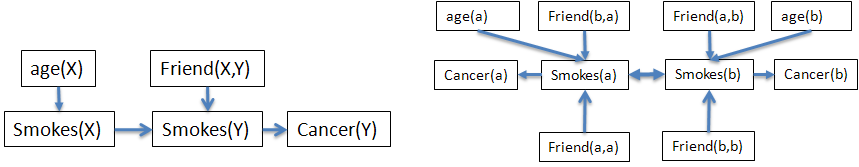
\includegraphics[width=1\textwidth]{double1.png}
}
\caption{A Bayes net with different predictors for $\it{Smokes}(\X)$ and $\it{Smokes}(\Y)$, and its grounding for two individuals $a$ and $b$.\label{fig:double}}
\end{center}
\end{figure}


%\begin{figure}[h]
%\begin{center}
%\resizebox{0.5\textwidth}{!}{
%\includegraphics{double}
%}
%\caption{An Bayes net with different predictors for $\it{Smokes}(\X)$ and $\it{Smokes}(\Y)$.\label{fig:double}}
%\end{center}
%\end{figure}
%
%If we treat $\it{Smokes}(\X)$ and $\it{Smokes}(\Y)$ as entirely separate variables, Bayes net learning needs to consider additional edges similar to those in the Bayes net, like \[\it{Smokes}(\X) \rightarrow \it{Cancer}(\X)\] and \[\it{age}(\Y) \rightarrow \it{Smokes}(\Y).\] Moreover, two edges like \[\age(X) \rightarrow \it{Smokes}(\X)\] and \[\age(\Y) \rightarrow \it{Smokes}(\Y)\] are redundant for the following reasons. (1) The population variables $\X$ and $\Y$ are interchangeable as they refer to the same entity set. (2) In terms of ground instances, the two edges connect exactly the same gnodes.


If we treat $\it{Smokes}(\X)$ and $\it{Smokes}(\Y)$ as entirely separate variables,  learning needs to consider additional edges similar to those already in the Bayes net, like $\it{Smokes}(\X) \rightarrow \it{Cancer}(\X)$ and $\it{age}(\Y) \rightarrow \it{Smokes}(\Y)$. However, such edges are redundant because the population variables $\X$ and $\Y$ are interchangeable as they refer to the same entity set. In terms of ground instances, the two exchanges connect exactly the same ground instances.
%
%\subsection{The Main Node and Main Variable Formats}
Redundant edges can be avoided if we restrict the model class to the main functor format, where for each function symbol $\functor$ (including relationships), there is a {\em main functor node} $\functor(\terms)$ such that all other functor nodes $\functor(\terms')$ associated with the same functor are sources in the graph, that is, they have no parents. 
%The intuition for this restriction is that statistically, two functors with the same function symbol are equivalent, so it suffices to model the distribution of these functors conditional on a set of parents just once. This leads to the following  definition.
%
%\begin{definition}
%A Bayes net $\B$ is in \textbf{main functor node form} if for every functor %symbol 
%$\functor$ of $\B$, there is a distinguished functor node $\functor(\terms)$, called the \textbf{main functor node} for $f$, such that every other functor node $\functor(\terms')$ for the same functor $\functor$ 
%%where $\terms' \neq \terms$, 
%has no parents in $\B$.
%\end{definition}
%Clause~\ref{clause:head} of Table~\ref{table:a2a} enforces the main variable format in the learn-and-join algorithm.
The term ``main functor node'' expresses that the main node is the main instance of functor $\functor$ from the point of view of modelling the conditional distribution of $\functor$. 
%One way to define main functor nodes is in terms of a lexicographic ordering derived from an ordering of population variables (cf. Section~\ref{sec:fnodes}). That is, the main node for function symbol $\functor$ is the functor $\functor(\term)$ where $\term$ is the lexicographically first list of terms for $\functor$. We refer to such Functor Bayes nets as
%\textbf{main variable} Functor Bayes nets. 

{\em Example.} The Bayes net of Figure~\ref{fig:pbn}, reproduced in Figure~\ref{fig:PBN-age}, is in main functor form. 
%The main functors are $\it{Friend}(\X,\Y)$ for the relationship predicate $\it{Friend}$, and $\it{Smokes}(\Y)$ for the function symbol $\it{Smokes}$, and $\it{Cancer}(\Y)$ for the function symbol $\it{Cancer}$. 
The Bayes net of Figure~\ref{fig:double} is not in main functor form because we have two functor nodes for $\it{Smokes}$ with nonzero indegree.
%For descriptive attributes of an entity, the corresponding functors that appear as child nodes all share a single variable (e.g., $\it{Cancer}(\X),\it{Smokes}(X)$); attribute functors with another variable may appear only as parents with indegree 0 and are used solely as auxilliary nodes to model recursive or auto-correlation relationships. Thus the main variable format helps to minimize the number of population variables used in Bayes net adjacencies. The Bayes net of Figure~\ref{fig:pbn} is in main variable form.

 \begin{figure}[h]
\begin{center}
\resizebox{1\textwidth}{!}{
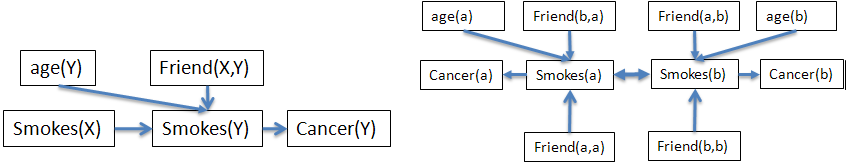
\includegraphics[width=1\textwidth]{single1.png}
}
\caption{An Bayes net in main variable format where $\it{Smokes}(\Y)$ is the main functor for $\it{Smokes}(\X)$. The ground Bayes net is the same as the ground Bayes net for the graph of Figure~\ref{fig:double}.\label{fig:PBN-age}}
\end{center}
\end{figure}


Schulte {\em et al.} \cite{Schulte2011a} provide a theoretical justification for the main functor node format by showing that under a mild assumption, every Bayes net $\B$ can be transformed into an equivalent Bayes net $\B'$ that is in main functor node form. It is easy to see that we can make {\em local} changes to the population variables such that all child nodes for a given functor are the same. For instance, in the Bayes net of Figure~\ref{fig:double} we can first substitute $\Y$ for $\X$ to change the edge $\age(X) \rightarrow \it{Smokes}(\X)$ into the edge $\age(\Y) \rightarrow \it{Smokes}(\Y)$. Then we delete the former edge and add the latter, that is, we make $\age(\Y)$ a parent of $\it{Smokes}(\Y)$. Figures~\ref{fig:double} and~\ref{fig:PBN-age} illustrate that the original and transformed Bayes nets have the same ground graph. However, in general the change of variables may introduce cycles in the Bayes net. The basis for the next proposition is that if the original Bayes net is stratified, the  transformed functor node graph is guaranteed not to contain cycles. 

A Functor Bayes Net is \textbf{stratified} if there is an ordering of the {\em functors} such that for every edge $\functor(\terms) \rightarrow g(\terms')$ in the Bayes net, either the functor symbol $\functor$ precedes the functor symbol $g$ in the ordering, or $\functor$ and $g$ are the same. Both Bayes nets in Figures~\ref{fig:double} and~\ref{fig:PBN-age} are stratified given the functor ordering $\it{age} > \it{Friend} > \it{Smokes} > \it{Cancer}$. 

\begin{proposition} \label{prop:normal}
Let $\B$ be a stratified Bayes net. Then there is a Bayes net $\B'$ in main functor form such that for every database $\D$, the ground graph $\ground{B}$ is the same as the ground graph $\ground{B'}$.
\end{proposition}

For the proof see \cite{Schulte2011a}. Stratification is a widely imposed condition on logic programs, because it increases the tractability of reasoning with a relatively small loss of expressive power \cite[Sec.3.5]{Lifschitz1996},\cite{Apt1991}. Related ordering constraints have also appeared in previous statistical-relational models  \cite{Fierens2009,Friedman99prm}. 


While the transformed Bayes nets have the same groundings, they are not equivalent at the variable or class level. For instance, in the model of Figure~\ref{fig:double} the maximum indegree is 2, whereas in the model of Figure~\ref{fig:pbn} the maximum indegree is 3. In effect, the transformation moves one or more parents from the auxilliary functor nodes to the main functor node, which produces larger families. In terms of Markov Logic Network clauses that result from moralization, the main functor format therefore leads to longer rules. 

\subsection{Population Variable Bound.} 
%We next discuss the bound on the relational complexity of a child-parent constellation, as measured by the number of population variables that appear in the constellation. 
As both the statistical and the computational complexity of Functor Bayes nets can be high, it is desirable to allow a user to specify a complexity bound to control the trade-off between expressive power and computational difficulty. A key issue is the length of the relationship chains 
%(foreign key chains, slot chains) 
that the algorithm needs to consider. The number of relationship chains grows exponentially with this  parameter. The computational complexity of computing sufficient statistics for a relationship set depends on the length of slot chains as well: with no bound on the length, the problem is \#P-complete \cite[Prop.12.4]{Domingos2007}.
We expect that more distantly related entities carry less information, so many SRL algorithms assume a small bound on the length of possible slot chains, on the order of 3 or so.
%[check this claim]
A less restrictive way to bound the complexity of relationship chains is to allow the user to specify a bound on the number of population variables that occur in a family (child + parent nodes), as proposed by Vardi \cite{Vardi1995}.
%Following a proposal of Vardi \cite{Vardi1995}, we allow the user to specify a bound on the number of population variables that occur in a family (child + parent nodes). 
Intuitively, this bounds the number of distinct (generic) objects that can be considered in a single child-parent configuration. 
%We emphasize that a variable number bound does not imply any bound on the length of clauses: even with a single population variable like $\S$ associated with students, we can have an arbitrary number of attributes of students in a single clause. Kok and Domingos \cite{Kok2010} highlight the importance of learning long clauses for relational models. 

%One possibility is to specify a bound on the number of parents of each node in an Bayes net. Vardi has proposed instead to bound the number of population variables that occur in a family (child + parent nodes).
%This implies a bound on the length of slot chains, but not on the number of parents of a node. For instance, we can add specifications of attribute values, and additional relationship nodes with the same population variables, without increasing the number of variables. 
With a constant bound on the number of variables, database frequencies involving these variables can be computed in polynomial time \cite{Vardi1995}. Khosravi {\em et al.} \cite{Khosravi2009} describe a dynamic programming algorithm for computing conditional probability parameters in a Functor Bayes Net that runs in polynomial time assuming a constant bound on the number of population variables in a family. 
%Our lattice search Algorithm~\ref{alg:structure} does not consider relationship sets that exceed the bound.
%%
%Algorithm~\ref{alg:structure} enforces the bound locally for each family.
%%dynamically during the local search.  
%An alternative is to enforce it globally by ensuring that the total number of population variables that occur in all functor random variables is bounded (cf. Section~\ref{sec:fnodes}).
%
%{\em Examples.} 
%The %relationship 
%chain $\it{Registered}(\S,\C),\it{TA}(\S,\C)$ has size 2 contains 3 variables. The %relationship 
%chain $\it{Likes}(\X,\Y),\it{Emails}(\X,\Y)$ has size 2 and contains 2 variables. This illustrates that adding relationships to a set does not necessarily increase the number of variables involved.

%An potential issue with the variable bound is that the maximally large relationship set may exceed it. For instance, in the University Schema example of Figure~\ref{table:university-schema}, the maximally large relationship set contains 3 variables, which  would exceed a bound of 2. In this case where
%%Even in the case where 
%the multi-net lattice contains more than one maximally large relationship set, the  lattice can be straightforwardly converted to other SRL formalisms as follows. Say that an Bayes net associated with a maximally large relationship set is maximal. 
%%In Figure~\ref{fig:big-lattice} there is only one maximally large relationship set with three members. 
%For Markov Logic Networks %, the focus of this paper, 
%we convert the maximal Bayes nets to MLNs using moralization; the union of these MLNs is the final output MLN. A multi-net lattice can similarly be converted to other clausal formalisms like BLPs and LBNs: A single Bayes net defines a set of directed clauses of the form $\it{child} \leftarrow \it{parents}$ and the union of these clauses over maximal Bayes nets defines the complete set. %The most complicated case arises 
%If an application requires a single Bayes net for the entire database, 
%%but the union of the maximal Bayes net graphs is not acyclic. In this case 
%it may be possible to apply a Bayes net combining algorithm to merge the maximal Bayes nets into a single one using BN merging algorithms \cite{Tillman2008}.


%\subsection{$\theta$-Equivalence Constraints}

% OS Nov 23. I was wrong to put this in. The problem is that after fixing the main functors, we may really need to consider relationships both ways. E.g., suppose that  in E-mails(X,Y), we have the main functor age(X). Then we need to consider Friend(X,Y) to find an edge from the sender to age(X), but also to consider Friend(Y,X) to find an edge from the receiver to age(X).

%Two functor sets $\set{\F}_{1},\set{\F}_{2}$ are statistically equivalent if they have the same cardinality and there is a 1-1 onto mapping $\pi$ from the population variables in $\set{\F}_{1}$ to the population variables in $\set{\F}_{2}$ such that the result of replacing each variable $\X$ in $\set{\F}_{1}$ with its image $\pi(\X)$ is  $\set{\F}_{2}$. This is a special case of $\theta$-equivalence as used by the \warmr system \cite{bib:query-ex}. Given the assumptions about functors from Section~\ref{sec:fnodes}, $\theta$-equivalence for binary relations is easy to check: If two functor lists are of different length, they are not $\theta$-equivalent. If they have the same length $k$, each functor list contains the  same number of argument positions (at most$2k$).
%% argument positions. 
%Say that $[\set{\F}_{1}$] \textbf{binds} a pair of positions if the same variable appears in both positions. Two functor lists $[\set{\F}_{1}],[\set{\F}_{2}]$ are $\theta$-equivalent if and only if they  bind the same positions.

%%
%% relationship sets $\set{\Relation}_{1},\set{\Relation}_{2}$ are statistically equivalent if they have the same cardinality and there is a 1-1 onto mapping $\pi$ from the population variables in $\set{\Relation}_{1}$ to the population variables in $\set{\Relation}_{2}$ such that the result of replacing each variable $\X$ in $\set{\Relation}_{1}$ with its image $\pi(\X)$ is  $\set{\Relation}_{2}$. This is a special case of $\theta$-equivalence as used by the \warmr system \cite{bib:query-ex}. Given the assumptions about relationship functors from Section~\ref{sec:fnodes}, $\theta$-equivalence for binary relations is easy to check: If two relationship lists are of different length, they are not $\theta$-equivalent. If they have the same length $k$, each relationship list contains $2k$ argument positions. Say that $[\set{\Relation}_{1}$] \textbf{binds} a pair of positions if the same variable appears in both positions. Two relationship lists $[\set{\Relation}_{1}],[\set{\Relation}_{2}]$ are $\theta$-equivalent if and only if they  bind the same positions.

%{\em Example.} The relationship chain \[\it{Friend}(\X,\Y),\it{Likes}(\Y,\X)\] is $\theta$-equivalent to the chain \[\it{Friend}(\Y,\X),\it{Likes}(\X,\Y).\]



%
%\section{Relationship Constraints}
%
%In this section we discuss the simpler constraints in Table~\ref{table:a2a} and the motivation for the variable bound.% then the main functor and lattice constraints.
%The two simplest constraints in Table~\ref{table:a2a} are Clause~\ref{clause:r2ra} and Clause~\ref{clause:rcontext}.
%Clause~\ref{clause:r2ra} models the deterministic impact of a relationship indicator variable $\Relation(\term)$ on each descriptive attribute $\functor_{\Relation}(\term)$ of the relationship: if $\Relation(\term) = \false$, then with probability 1, $\functor_{\Relation}(\term) = \bot$. Clause~\ref{clause:rcontext} says that if an association between attributes $\functor(\terms) \rightarrow g(\terms')$ depends on the relational context $\set{\Relation}$, then the Bayes net must include the relationship functors in $\set{\Relation}$ as parents of $g(\terms')$ in order to indicate the context-dependence. 
%The remaining constraints of Table~\ref{table:a2a} are more complex and we discuss them in detail in the following sections. 
%The constraints on relationship chains are of two types. (1)

%(2) Statistical equivalence constraints: Viewed as random variables, two population variables $\X,\Y$ that are associated with the same population behave exactly the same: they are identically distributed, and so are two functor nodes with the same function symbol, e.g., $\f(\X),\f(\Y)$. However, in an Bayes net these random variables correspond to distinct nodes and hence learning algorithms treat them separately, which leads to duplication of learning effort, unless further constraints are imposed.
%(3) Lattice constraints: Propate the presence or absence of edges from smaller relationship sets to larger ones. These enforce the general principle of evaluating statistical associations in minimal contexts. We discuss and motivate the constraints in turn.



%

%

%{\em Example.}

%%The functor concept allows different nodes in an Bayes net to be associated with the same attribute or relationship, where the difference between these functors is in their variable arguments only. This expressive power is essential to represent recursive dependencies where instances of an attribute/relationship depend on other instances of the same attribute/relationship. However, it causes additional complexity in learning if each functor is treated as a separate random variables. Consider for example the Bayes net shown in Figure~\ref{fig:double}.

%%  \begin{figure}[h]
%%\begin{center}
%%\resizebox{0.7\textwidth}{!}{
%%\includegraphics[width=0.7\textwidth]{double}
%%}
%%\caption{A Bayes net with different predictors for $\it{Smokes}(\X)$ and $\it{Smokes}(\Y)$.\label{fig:double}}
%%\end{center}
%%\end{figure}

%If we treat $\it{Smokes}(\X)$ and $\it{Smokes}(\Y)$ as entirely separate variables, Bayes net learning needs to consider multiple equivalent edges, like $\it{Cancer}(\X) \rightarrow \it{Smokes}(\X)$ and $\it{Cancer}(\Y) \rightarrow \it{Smokes}(\Y)$. In terms of the grounding semantics, these edges have exactly the same groundings.
%To avoid such redundancy, we restrict the model class to the head functor format, where for each function symbol $\functor$ (including relationships), there is a main or head functor $\functor(\terms)$ such that all other functors $\functor(\terms')$ associated with the same function symbol are sources in the graph, that is, they have no parents. The intuition for this restriction is that since two functors with the same function symbol are statistically equivalent, it suffices to model the distribution of these functors conditional on a set of parents just once. This leads to the following definition.

%\begin{definition}
%A Bayes net $\B$ is in \textbf{head functor form} if for every function or predicate symbol $f$ of $\B$, there is a distinguished functor $\functor(\terms)$, called the \textbf{head functor} for $f$, such that every other functor $\functor(\terms'), \terms' \neq \terms$ has no parents in $\B$.
%\end{definition}

%In what follows we assume that the head functors are derived from a lexicographic ordering of the functors (cf. Section~\ref{sec:pbns}). That is, the head functor for function symbol $\functor$ is the functor $\functor(\term)$ where $\term$ is the lexicographically first list of terms for $\functor$.
%%It can be shown that the normal form result for stratified Bayes nets extends to head functors defined lexicographically.
%The term ``head functor'' expresses that the head functor is the main instance of function $f$ from the point of view of modelling the conditional distribution of $f$. It also derives from the concept of the head of a rule in Logic Programming (LP), where the head is the consequent of a rule of the form $\it{head} \leftarrow \it{body}$. In terms of rules, the head functor format requires that for each function symbol $\functor$, only one functor $\functor(\terms)$ associated with $\functor$ appears as the head of any rule.
%%

The next section presents empirical evidence about the performance of the learn-and-join algorithm on benchmark datasets.



\section{Evaluation: Experimental Design}
%All experiments were done on a QUAD CPU Q6700 with a 2.66GHz CPU and 8GB of RAM. For single table Bayes net search we used GES search \cite{Chickering2003} with the BDeu score as implemented in version 4.3.9-0 of CMU's Tetrad package (structure prior uniform, ESS=10; \cite{2008a}). Our code and datasets are available for anonymous ftp download \cite{bib:jbnsite}.
%%Default structure learning, weight learning and the MC-SAT inference algorithm \cite{Poon2006} of the Alchemy package were also used.

All experiments were done on a QUAD CPU Q6700 with a 2.66GHz CPU and 8GB of RAM. Our code and datasets are available on the world-wide web \cite{bib:jbnsite}. We made use of the following existing implementations.

 \begin{description}
\item[\textbf{Single Table Bayes Net Search}]  GES search \cite{Chickering2003} with the BDeu score as implemented in version 4.3.9-0 of CMU's Tetrad package (structure prior uniform, ESS=10; \cite{2008a}).
\item [\textbf{MLN Parameter Learning}] The default weight training procedure \cite{Lowd2007} of the Alchemy package \cite{Kok2009a}, Version 30.
\item [\textbf{MLN Inference}] The MC-SAT inference algorithm \cite{Poon2006} to compute a probability estimate for each possible value of a descriptive attribute for a given object or tuple of objects. 
\item [\textbf{Join Data Tables}] The join data tables for a given relationship chain are computed using a straightforward SQL inner join over the required relationship and entity tables. Our database management system is MySQL Version 1.2.15.
\end{description}

The computation of the join data tables could be optimized in a number of ways. For instance, like most Bayes net scores, the BDeu score requires only the sufficient statistics, or database frequencies of events. Rather than materializing the entire join data table, we could use indices or the SQL $\it{Count}$ aggregate function to compute these summary statistics only. We did not include optimizations of the database computations because data management is not the focus of our paper, and we already achieve very fast learning without them. Thus the database is used only to find the set of tuples that satisfy a given joint condition (e.g., find the set of $(x,y)$ pairs such that $\it{Friend}(\X,\Y) = \true, \it{Smokes}(\X) = \true, \it{Smokes}(\Y) = \false$).

%don't forget Flavia's idea for subsampling
\subsection{Datasets} 
\label{sec:datasets}
We used two synthetic and five benchmark real-world datasets for our evaluation.%\marginpar{Add a note that we select datasets for different parts of the study} 


\paragraph{University Database.} We manually created a small dataset, based on the schema given in Table~\ref{table:university-schema}.
%The dataset is small and is used as a purpose of proofing the correctness of our algorithms.
The entity tables contain 38 students, 10 courses, and 6  Professors. The $\reg$ table has 92 rows and the $\it{RA}$ table has 25 rows. %This dataset is translated into 513 ground atoms.

\paragraph{University+ Database.} To test learning algorithms with autocorrelations, we extended this database with a self-relationship $\it{Friend}$ between Students and several descriptive attributes of students, such that the ranking and coffee drinking habits of a student are strongly correlated with the ranking and coffee drinking habits of her friends, respectively. 

\paragraph{MovieLens Database.} The MovieLens dataset is from the UC Irvine machine learning repository. %The schema for the dataset is shown in Table \ref{}.
It contains two entity tables: $\it{User}$ with 941 tuples and $\it{Item}$ with 1,682 tuples, and one relationship table $\it{Rated}$ with 80,000 ratings. The $\it{User}$ table has %key field $\it{user\_id}$ and
3 descriptive attributes $\age, \it{gender}, \it{occupation}$. We discretized the attribute age into three bins with equal frequency. The table $\it{Item}$ represents information about the movies. It has 17 Boolean attributes that indicate the genres of a given movie. We performed a preliminary data analysis and omitted genres that have only weak correlations with the rating or user attributes, leaving a total of three genres.

% The full dataset contains 170143 ground atoms and is too big for MLN to do structure learning or parameter learning on. We made small subsamples to make the experiments feasible. Sub sampling 100 Users and 100 Items transforms to a db file with 2505 number of groundings. takes around 30 min to run. Sub sampling 300 Users and 300 Items transforms to a db file with 18040 number of groundings takes around 2 days to run.
%The full table with 100,000 ratings exceeded the memory limits of Tetrad, so we randomly picked 40\% of the ratings of the relationship table as input data.

\paragraph{Mutagenesis Database.} This dataset is widely used in ILP research \cite{Srinivasan1996}. %It contains 4 tables total to 15218 tuples.
Mutagenesis has two entity tables, $\it{Atom}$ with 3 descriptive attributes, and $\it{Mole}$, with %188 entries and
5 descriptive attributes, including two attributes that are discretized into ten values each (logp and lumo). It features two relationships $\it{MoleAtom}$ indicating which atoms are parts of which molecules, and $\it{Bond}$ which relates two atoms and has 1 descriptive attribute. %The full dataset, with 35973 ground atoms, crashed while doing either parameter learning or structure learning. A subsample with 5017 ground atoms is used was running for 5 days and did not terminate. weight learning was feasible. another subsample with
%Representing a relationship between entities from the same table in a parametrized Bayes net requires using two or more variables associated with the same population (e.g., $\it{Bond}(\A_{1},\A_{2}))$.

% problem: Bahareh changed the dataset so that there is a binary relationship Bond(Mole, Atom). Is it the case that for a given mole and atom, there is only one bond type? And the atom is related only to one other atom?

%\paragraph{ Financial Database.} The third dataset is a modified version of the financial dataset from the PKDD 1999 cup. % used in \cite{}.
%We adapted the database design to fit the ER model. We have two entity tables: $\it{Client}$ with 5369 tuples and $\it{Account}$ with 4,500 tuples. Two relationship tables, $\it{CreditCard}$ with 5,369 tuples and $\it{Disposition}$ with 892 tuples relate  a client with an account.
%The Client table has 10 descriptive attributes: the client's age, gender and 8 attributes on demographic data of the client. The Account table has 3 descriptive attributes: information on loan amount associated with an account, account opening date, and how frequently the account is used.

\paragraph{Hepatitis Database.} This dataset is a modified version of the PKDD�02 Discovery Challenge database. We adopted the modifications of Frank {\em et al.} \cite{Frank2007}, which includes removing tests with null values. It contains data on the laboratory examinations
of hepatitis B and C infected patients. The examinations were realized between 1982 and 2001 on 771 patients. The data are organized in 7 tables (4 entity tables,  3 relationship tables and 16 descriptive attributes). They contain basic information about the patients, results of biopsy, information on interferon therapy, results of out-hospital examinations, results of in-hospital examinations. 
%This dataset is challenging for Alchemy's structure learning, which terminated neither on the original dataset nor on a subsample of about 60\% size.

\paragraph{Mondial Database.}  This dataset contains data from multiple geographical web data sources \cite{mondial}. We follow the modification of \cite{wangMondial}, and use a subset of the tables and features. Our dataset includes a self-relationship table  $\it{Borders}$ that relates two countries.
% which introduces Autocorrelation. 

\paragraph{UW-CSE database.} This dataset lists facts about the Department of Computer Science and Engineering at the University of Washington (UW-CSE) (e.g., Student, Professor) and their relationships (i.e. AdvisedBy, Publication). 
%The total number of ground atoms is 4,106,841. The database contained a total of 3380 ground atoms. 
The dataset was obtained  by crawling pages in the department's Web site (www.cs.washington.edu). Publications and AuthorOf relations were extracted from the BibServ database (www.bibserv.org). 

 Table~\ref{table:datasetsize} lists the  databases and their sizes in terms of total number of tuples and number of ground atoms, which is the input format for Alchemy.

\begin{table}[tbp] \centering
%\scalebox{0.7in}{
\resizebox{0.6\textwidth}{!}{
\begin{tabular}[c]
{|l|l|l|}\hline
 \textbf{Dataset} & \textbf{\#tuples} & \textbf{\#Ground atoms} \\\hline
University&171&513\\\hline
Movielens &82623&170143\\\hline
Mutagenesis &15218& 35973 \\\hline
Hepatitis &12447&71597 \\\hline
Mondial &814&3366 \\ \hline
UW-CSE &2099&3380 \\ \hline
\end{tabular}
}
%} % end scalebox
\caption{Size of datasets in total number of table tuples and ground atoms. Each descriptive attribute is represented as a separate function, so the number of ground atoms is larger than that of tuples.  \label{table:datasetsize}}
\end{table}

Because several of the Alchemy systems returned no result on some of the real-world datasets, we formed two subdatabases for each by randomly selecting entities for each dataset. We restricted the relationship tuples in each subdatabase to those that involve only the selected entities. Table \ref{Tab:subdatabase} lists the resulting subdatabases and their sizes in terms of total number
of tuples and number of ground atoms.



\begin{table}[tbp] \centering
%\scalebox{0.7in}{
\resizebox{0.7
\textwidth}{!}{
\begin{tabular}[c]
{|l|l|l|}\hline
 \textbf{Dataset} & \textbf{\#tuples} & \textbf{\#Ground atoms} \\\hline
MovieLens1 (subsample)&1468&3485\\\hline
MovieLens2 (subsample)&12714 &27134 \\\hline
Mutagenesis1 (subsample)&3375& 5868\\\hline
Mutagenesis2 (subsample)&5675&9058 \\\hline
Hepatitis1 &6162 & 41335 \\\hline
\end{tabular}
}
%} % end scalebox
\caption{Size of subdatasets in total number of table tuples and ground atoms. Each descriptive attribute is represented as a separate function, so the number of ground atoms is larger than that of tuples.  \label{Tab:subdatabase}}
\end{table}



\subsection{Graph Structures Learned by the Learn-and-Join algorithm}

%In these datasets, there is a unique maximal relationship set, and hence a unique output Bayes net.
Figure~\ref{fig:struct} shows the learned Bayes nets for the University, Hepatitis, MovieLens, and Mondial datasets. The graphs illustrate how the learn-and-join algorithm learns models with complex dependency patterns. 


\begin{figure}[htbp] %  figure placement: here, top, bottom, or page
   \centering
     \resizebox{1.2\textwidth}{!}{
   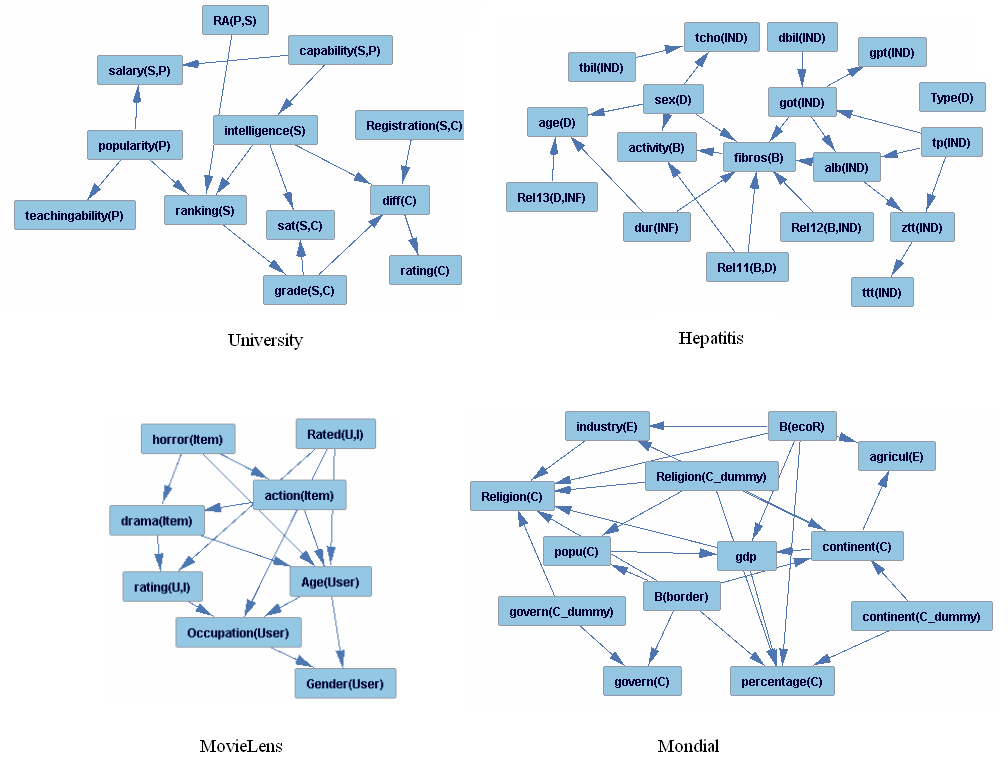
\includegraphics{mixBayesNets.png}
   }
   \caption{The Bayes net structures learned by the learn-and-join algorithm for 4 datasets. We omitted edges from Boolean relationship nodes to descriptive attributes of the relationship to make the figure more easily readable.}
   \label{fig:struct}
\end{figure}



%\begin{figure}[htbp] %  figure placement: here, top, bottom, or page
%   \centering
%     \resizebox{0.5\textwidth}{!}{
%   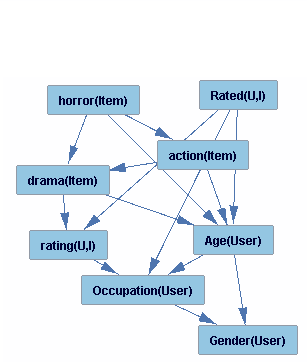
\includegraphics{movie}
%   }
%   \caption{The Bayes net structure learned by the learn-and-join algorithm for the MovieLens Dataset.}
%   \label{fig:structmovie}
%\end{figure}
%
%\begin{figure}[htbp] %  figure placement: here, top, bottom, or page
%   \centering
%   \resizebox{0.7\textwidth}{!}{
%   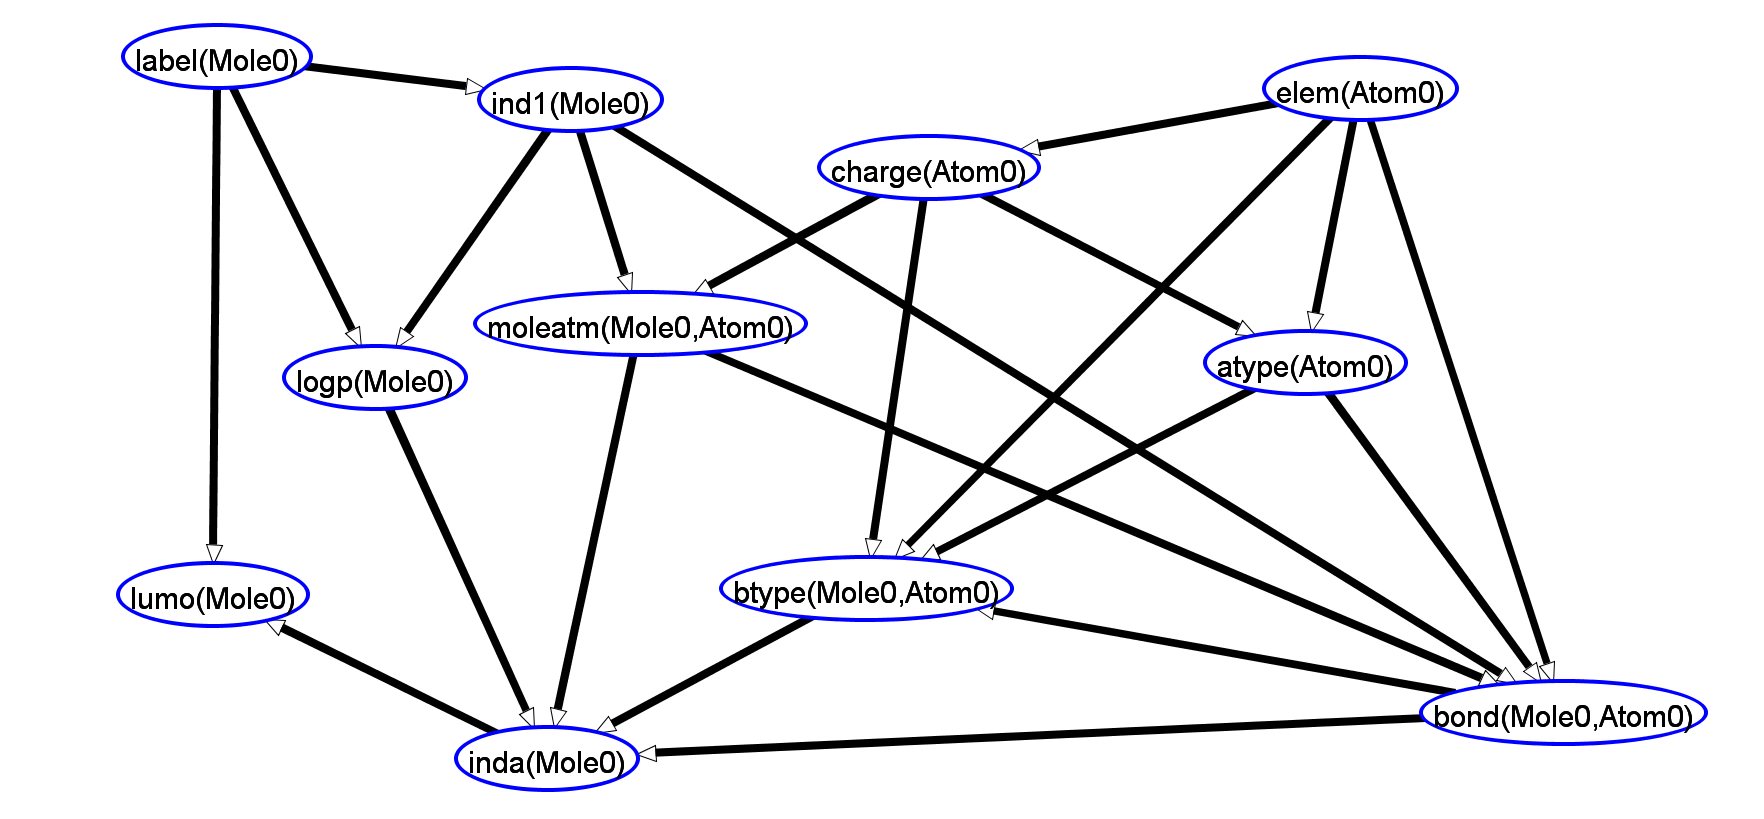
\includegraphics{muta.png}
%   }
%   \caption{The Bayes net structure learned by the learn-and-join algorithm for the Mutagenesis Dataset.}
%   \label{fig:structmuta}
%\end{figure}
%
%\begin{figure}[htbp] %  figure placement: here, top, bottom, or page
%   \centering
%   \resizebox{0.7\textwidth}{!}{
%   \includegraphics{hep.png}
%   }
%   \caption{The Bayes net structure learned by the learn-and-join algorithm for the Hepatitis Dataset. }
%   \label{fig:structhepa}
%\end{figure}

%
%\begin{figure}[h] %  figure placement: here, top, bottom, or page
%   \centering
%   \resizebox{0.7\textwidth}{!}{
%   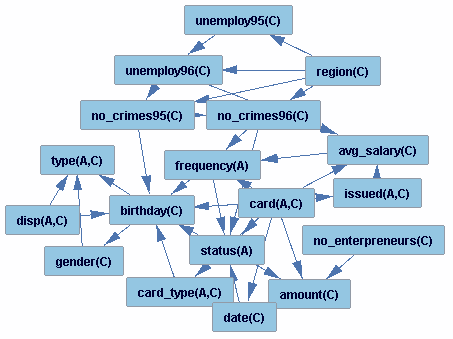
\includegraphics{financial1}
%   }
%   \caption{The Bayes net structure learned by the learn-and-join algorithm for the Financial Dataset.}
%   \label{fig:structfinancial}
%\end{figure}


\section{Moralization vs. Other Structure Learning Methods: Basic Comparisons}
\label{sec:basic-eval}

We begin with a set of comparisons on standard benchmarks that follows the design and  performance metrics of previous MLN structure learning studies \cite{Khosravi2010,Mihalkova2007,Kok2009}. Then we focus on experiments that assess specific components of the learn-and-join algorithm.

\subsection{Comparison Systems and Performance Metrics}

%We refer to the output of the learn-and-join Algorithm~\ref{alg:structure} as MBNs. Weight learning is carried out with Alchemy's default procedure, which currently uses the method of Kok and Domingos \cite{Kok2005a}.
 %, so that our parametrization method is comparable to that of Alchemy's in terms of runtime and quality.
We compared the learn-and-join algorithm with 4 previous Markov Logic Network structure learning methods implemented in different versions of Alchemy.

\begin{description}
\item [\textbf{MBN}] uses the learn-and-join algorithm to learn a Functor Bayes net. To perform inference, the Functor Bayes net is converted to a Markov Logic Network using moralization, which we refer to as the Moralized Bayes Net (see Section~\ref{sec:background}). Weights for the moralized Bayes net are learned using Alchemy's weight learning routine.
	\item[\textbf{$\MLNA$}] uses beam search which begins by adding unit clauses to an Markov Logic Network. $\MLNA$ then considers all clauses of length two and always maintains the $n$ highest-scoring ones
in the set. MSL terminates when it cannot find a clause that improves upon the current Markov Logic Network's score \cite{Kok2005a}.
	\item[\textbf{$\LHL$}] Lifted Hypergraph Learning \cite{Kok2009} uses relational path finding to induce a more compact representation of data, in the form of a hypergraph over clusters of constants. Clauses represent associations among the clusters.
	\item[\textbf{$\BUSL$}] Applies relational path finding to ground atoms and variabilizes each ground atom in a path. It then constructs a Markov network for the nodes in the path, then computes a single data table for the path and learns edges between the nodes using a single-table Markov network learner
%	viewed as Boolean variables and uses a Grow-Shrink Markov network learning algorithm to find the edges between the nodes using $\chi^2$ measure. 
	\cite{Mihalkova2007}.
\item[\textbf{LSM}]  Learning Structural Motifs \cite{Kok2010} uses random walks to identify densely connected objects in data, and groups them and their associated relations into a motif.
\end{description}


%Data reformatting was used by Kok and Domingos \cite{Kok2007}. To illustrate, for instance the predicate $\it{Salary}$ with values(high, medium, low), is represented with a single binary predicate $\it{Salary}(Student, Salary\_Type)$ in the standard Alchemy input format. The reformatted file contains instead three unary predicates \[\it{Salary}_{\it{high}}(\it{Student}), \it{Salary}_{\it{med}}(\it{Student}), \it{Salary}_{\it{low}}(\it{Student}).\] The effect is that the arguments to all predicates are primary keys, which tends to yield better results with Alchemy.
%To evaluate predictions, the Markov Logic Networks learned with the reformatted data were converted to the format of the original database.

 We use 3 performance metrics:  Runtime, Accuracy, and Conditional log likelihood. These measures have been used in previous studies of Markov Logic Network learning \cite{Mihalkova2007,Kok2009,Khosravi2010}. 
 
{\begin{description}
	\item[\textbf{Runtime}] The time taken to learn the model from the training dataset. 
	\item [\textbf{Accuracy (ACC)}] is the percentage of the descriptive attribute values that are correctly predicted by the Markov Logic Network.
	\item[\textbf{Conditional Log-Likelihood (CLL)}] The conditional log-likelihood of a ground atom in a database $\D$ given an Markov Logic Network is its log-probability given the Markov Logic Network and $\D$. The CLL directly measures how precise the estimated probabilities are.
\end{description}
 
%The AUC curves were computed by changing the CLL threshold above which a ground atom is predicted true (10 tresholds were used). The AUC is insensitive to a large number of true negatives. 
For ACC and CLL the values we report are averages over all attribute predicates. Khosravi {\em et al.} also report the AUC (area-under-curve) for predicates that correspond to descriptive attributes with binary values (e.g. gender), for the databases MovieLens and Mutagenesis \cite{Khosravi2010}. As there are only few binary descriptive attributes, we omit AUC from this study. For the existing binary predicates, the AUC improvement of the MBN approach over previous Markov Logic Network methods is similar to that for ACC and CLL.
%For AUC, it is the average over all attribute predicates that correspond to descriptive attributes with binary values (e.g. gender).  



\subsection{Runtime Comparison}

Table \ref{table:compare} shows the time taken in minutes for learning in each dataset. The Alchemy times include both structure and parameter learning. For the MBN approach, we report both the Bayes net structure learning time and the time required for the subsequent parameter learning carried out by Alchemy. 

\begin{table}[htbp] \centering
%\scalebox{0.8}
%\resizebox{0.7\textwidth}{!}{
\begin{tabular} [c]
{|l|l|l|l|l|l|} 
\hline &\multicolumn{4}{|c|}{Alchemy Methods}& LAJ
%\multicolumn{2}{|c|}{Moralization}
\\
\hline
 \textbf{Dataset}  & \textbf{\MLNA} &   \textbf{\LHL} & \textbf{BUSL}  &\textbf{ LSM} & \textbf{MBN} \\\hline
University & 5.02 &3.54& 0.5 &\textbf{0.01} &\textbf{0.03 + 0.032}\\\hline
MovieLens  &NT&NT &NT&\textbf{ 0.45} &\textbf{1.2 +120	 }\\\hline
MovieLens1 & 44& 34.52& 50 & \textbf{0.03} &\textbf{0.05 + 0.33 }\\\hline
MovieLens2 & 2760 & 3349& NT& \textbf{0.06} &\textbf{0.12 + 5.10 }\\\hline
Mutagenesis  &NT&NT&NT&\textbf{0.53} &0.5 + 106\\\hline
Mutagenesis1  &3360&  3960 &150 & \textbf{0.12}& \textbf{0.1 + 5  }\\\hline
Mutagenesis2  &NT& NT&NT& \textbf{0.17}&\textbf{0.2 +12 }\\\hline
Hepatitis &NT&NT&NT&\textbf{0.15}&\textbf{0.4 + 95.6  }\\\hline
Hepatitis1 &NT&NT&NT&\textbf{0.1}&\textbf{0.2 + 4.8}\\\hline
\end{tabular}
%} % end scalebox
\caption{Runtime to produce a parametrized Markov Logic Network, in minutes. The MBN column shows structure learning time + weight learning time. NT indicates non-termination. \label{table:compare}}
\end{table}

%\begin{table}[tbph] \centering
%\resizebox{0.7\textwidth}{!}{
%\begin{tabular} [c]
%{|l|l|l|l|l|l|}\hline
% \textbf{Dataset} & \textbf{MBN} & \textbf{\MLNA} & \textbf{\MLNConst} & \textbf{\LHL} &\textbf{\LHLConst} \\\hline
%University& 0.03 + 0.032 & 5.02 &11.44 &3.54& 19.29 \\\hline
%MovieLens &1.2 +120&NT&NT & NT& NT \\\hline
%MovieLens1& 0.05 + 0.33 & 44& 121.5&34.52&126.16\\\hline
%MovieLens2& 0.12 + 5.10 & 2760 & 1286 & 3349& NT\\\hline
%Mutagenesis &0.5 +NT&NT&NT&NT&NT\\\hline
%Mutagenesis1 &0.1 + 5&3360& 900& 3960 &1233\\\hline
%Mutagenesis2 &0.2 +12 &NT&3120&NT& NT\\\hline

%\end{tabular}
%} % end scalebox
%\caption{Runtime to produce a parametrized MLN, in minutes. The MBN column shows structure learning time + weight learning time. \textbf{Add Financial?}\label{table:compare}}
%\end{table}

%{\em Structure Learning.} The learn-and-join algorithm returns an MLN structure very quickly (under 2 minutes).
%This includes single-table BN parameter estimation as a subroutine.

%\paragraph{Structure and Weight Learning.}
{\em Structure learning is very fast for both the MBN and the LSM method}, orders of magnitude faster than for the other methods.
The total runtime for MBN is dominated by the time required by Alchemy to find a parametrization for the moralized Bayes net. On the smaller databases, this takes between 5-12 minutes. On MovieLens, parametrization takes two hours, and on Mutagenesis, over 1.5 hours. %and Financial, 
%it does not terminate. 
While finding optimal parameters for the MBN structures remains challenging, the combined structure+weight learning system is much faster than the overall structure + weight learning time of most of the Alchemy methods: They do not scale to the complete datasets, and for the subdatabases, the MBN approach is faster by a factor ranging from 200 to 1000. 

These results are strong evidence that the MBN approach leverages the scalability of Bayes net learning to achieve scalable Markov Logic Network learning on databases of realistic size. The LSM method is very fast for all datasets. Inspection of the learned clauses by LSM  shows that the rules are mostly just the unit clauses that model  marginal probabilities. This indicates underfitting the data, as the following measurements of accuracy and conditional log-likelihood confirm.
%
%As reported by Kok and Domingos \cite{Kok2009}, the runtimes reported on other smaller databases for other Markov Logic Network learners
%are also much larger (e.g., \textsc{BUSL} takes about 13 hr on the UW-CSE dataset with 2,112 ground atoms).



\subsection{Predictive Accuracy and Data Fit}

Previous work on Markov Logic Network evaluation has used a ``leave-one-out'' approach that learns Markov Logic Networks for a number of subdatabases with a small subset omitted \cite{Mihalkova2007}. This is not feasible in our setting
%for databases with many descriptive attributes
because even on a training set of size about 15\% of the original, finding an Markov Logic Network structure using the slower Alchemy methods is barely possible. Given these computational constraints, we investigated the predictive performance by learning an Markov Logic Network on one randomly selected 2/3 of the subdatabases as a training set, testing predictions on the remaining 1/3.  While this does not provide strong evidence about the
generalization performance in absolute terms, it gives information about the relative performance of the methods. In the next section we give further cross validation results using the fastest Alchemy methods LSM and LHL. Tables~\ref{results} and~\ref{tabletest:CLL} report the average accuracy and conditional log-likelihood of each real-world dataset. (The synthetic dataset University was too small for learning on a subset). %and AUC 
%of each dataset except Financial. 
%We left out Financial because even smaller subdatabases were infeasible for the Alchemy structure and parameter learning algorithms. 
Higher numbers indicate better performance and NT indicates that the system was not able to return an Markov Logic Network for the dataset, either crashing or timing out after 4 days of running. {\em MBN achieved substantially better predictions on all test sets, in the range of 10-20\% for accuracy.} 

The CLL performance of LSM is acceptable on average. The parameter estimates are biased towards uniform values, which leads to predictions whose magnitudes are not extreme. Because the average accuracy is low, this means that when mistaken predictions are made, they are not made with great confidence. The LSM pattern of low accuracy and acceptable log-likelihood is found in our other datasets as well.



\begin{table}[tph] \centering
%{\small
 %\resizebox{1\textwidth}{!}{
\begin{tabular} [c]
%{|l|l|l|l|l|l|l|l|l|l|llllll}\hline
{|c|c|c|c|c|c|c|c|c|} \hline
Accuracy &\multicolumn{4}{|c|}{Alchemy Methods}&LAJ\\\hline
 \textbf{Dataset}  & \textbf{\MLNA} &   \textbf{\LHL} & \textbf{BUSL}  &\textbf{ LSM} & \textbf{MBN} \\\hline
Movielens11& 0.40&  0.42&0.34 & 0.37& \textbf{0.63}\\\hline
Movielens12& 0.41&  0.44&NT& 0.49& \textbf{0.62}\\\hline
Movielens& NT & NT&NT& 0.30& \textbf{0.69}\\\hline
Mutagenesis1& 0.34&0.31&0.37&0.30 & \textbf{0.69}\\\hline
Mutagenesis2& NT&0.35&NT& 0.28& \textbf{0.65}\\\hline
Hepatitis &NT &NT&NT&0.32& \textbf{0.54}\\\hline
Hepatitis1 &NT &NT&NT&0.29 & \textbf{0.53}\\\hline
\end{tabular}
%} % end scalebox
\caption{The table compares accuracy performance of the moralization approach (MBN) vs. previous Markov Logic Network learning methods. The data are obtained by training on 2/3 of the database and testing on the other 1/3. ACC is reported as an average over all attribute predicates of the datasets.
\label{results}}
\end{table}

\begin{table}[thpb] \centering
% \resizebox{1\textwidth}{!}{
\begin{tabular} [c]
%{|l|l|l|l|l|l|l|l|l|l|llllll}\hline
{|c|c|c|c|c|c|c|} \hline
Conditional Log-likelihood &\multicolumn{4}{|c|}{Alchemy Methods}&LAJ\\
\hline
\textbf{Dataset}  & \textbf{\MLNA} &   \textbf{\LHL} & \textbf{BUSL}  &\textbf{ LSM} & \textbf{MBN} \\\hline
Movielens11&-4.22&-4.60&-2.80&-1.21& \textbf{-1.15}\\\hline
Movielens12&-3.55&-3.38&NT&\textbf{-1.06} & -1.33\\\hline
Movielens&NT&NT&NT&-1.1& \textbf{-0.98 }\\\hline
Mutagenesis1&-4.45&-4.33&-2.54& \textbf{-1.12}&-1.85\\\hline
Mutagenesis2 &NT &NT&NT& \textbf{-1.18}&-1.48\\\hline
Hepatitis &NT &NT&NT&-1.26 & \textbf{-1.18}\\\hline
Hepatitis1  &NT&NT&NT&-1.34& \textbf{-1.09}\\\hline
\end{tabular}
%} % end scalebox
\caption{The table compares conditional log likelihood performance of the moralization approach (MBN) vs. previous Markov Logic Network learning methods. The data are obtained by training on 2/3 of the database and testing on the other 1/3. CLL is reported as an average over all attribute predicates of the datasets. \label{tabletest:CLL}}
\end{table}


Where the learning methods return a result on a database, we also measured the
predictions
%data fit
of the different Markov Logic Network models
%by checking how well they predict
for the facts in the training database. This indicates how well the Markov Logic Network summarizes the statistical patterns in the data. %, and does not require selecting a subdatabase.
%These metrics have several advantages. (1) They do not require selecting a subdatabase. (2) Because of the complexity of relational databases, a compact summary of the database statistics is valuable. Research has shown that a model trained on the entire database can effectively support applications like query execution planning \cite{Getoor2001}. (3) The learn-and-join method learns a model of type 1 probabilities; even if such a model were to exactly reproduce the database frequencies, there are different ways to derive type 2 instance-level predictions from it.
%The most common way for parametrized Bayes nets is to employ combining rules \cite{Poole2003}.
These measurements test the log-linear equation~\eqref{eq:log-linear} as a solution to the combining problem for inference (see Section~\ref{sec:background}). While a small improvement in predictive accuracy may be due to overfitting, the very large improvements we observe are evidence that the Markov Logic Network models produced by the Alchemy methods underfit and fail to represent statistically significant dependencies in the data. Tables~\ref{results-notest} and~\ref{table:cll-notest} show the results for Accuracy and Conditional Log-likelihood.
{\em MBN achieved substantially better predictions on all test sets, at least 20\% for accuracy.}

%
%\begin{table}[tph] \centering
%%{\small
% \resizebox{1\textwidth}{!}{
%\begin{tabular} [c]
%%{|l|l|l|l|l|l|l|l|l|l|llllll}\hline
%{|c|c|c|c|c|c|c|c|c|c|c|c|c|c|c|c|} \hline
% \textbf{Dataset} &  \multicolumn{5}{c|}{\textbf{Accuracy}} &  \multicolumn{5}{c|}{\textbf{CLL}} & \multicolumn{5}{c|}{\textbf{AUC} }\\\hline
%&MBN&\MLN&\MLNConst & \LHL & \LHLConst& MBN&\MLN&\MLNConst & \LHL & \LHLConst & MBN&\MLN&\MLNConst &\LHL & \LHLConst\\\hline
%Movielens11 & \bf{0.63} & 0.39 & 0.45 & 0.42& 0.50& \bf{-0.99} & -3.97 & -3.55 & -4.14& -3.22& \bf{0.64}& 0.46 & 0.60 & 0.49&0.55 \\\hline
%Movielens12 & \bf{0.59} & 0.42 & 0.46 & 0.41& NT &\bf{-1.15} & -3.69 & - 3.56 & -3.68& NT& \bf{0.62} & 0.47 &0.54 & 0.50&NT \\\hline
%Mutagenesis1  & \bf{0.60} & 0.34 & 0.47 & 0.33 & 0.45 &  \bf{-2.44} & -4.97 & - 3.59 & -4.02& -3.12& \bf{0.69} & 0.56 &0.56 & 0.50 &0.53 \\\hline
%Mutagenesis2 & \bf{0.68} & NT & 0.53 & NT & NT& \bf{-2.36} & NT & - 3.65 & NT& NT & \bf{0.73} & NT & 0.59 & NT & NT \\\hline
%\end{tabular}
%} % end scalebox
%\caption{The table compares the predictive performance of the moralization approach (MBN) vs. previous MLN learning methods. The data are obtained by training on 2/3 of the database and testing on the other 1/3. \textbf{missing BUSL}
%\label{results}}
%\end{table}
%

%\begin{table}[tphb] \centering
% \resizebox{1\textwidth}{!}
%{
%\begin{tabular} [c]
%%{|l|l|l|l|l|l|l|l|l|l|llllll}\hline
%{|c|c|c|c|c|c|c|c|c|c|} \hline
% &\multicolumn{5}{|c|}{Alchemy Methods}&LAJ\\
%\hline
% \textbf{Dataset}&\MLN&\MLNConst & \LHL & \LHLConst & BUSL & MBN   \\\hline
%University & 0.37& 0.51& 0.37&0.55&0.38&0.84\\\hline
%Movielens11& 0.43& 0.43 & 0.42&0.49&0.36& 0.69\\\hline
%Movielens12& 0.42& 0.42 & 0.48&0.57&NT& 0.68 \\\hline
%Movielens& NT & NT& NT& NT&NT& 0.74\\\hline
%Mutagenesis1& 0.36& 0.55&0.33&0.52&0.37& 0.80\\\hline
%Mutagenesis2& NT&0.35&NT&NT&NT& 0.65\\\hline
%Hepatitis&NT &NT&NT&NT&NT&0.57 \\\hline
%Hepatitis1 &NT &NT&NT&NT&NT& 0.57\\\hline
%\end{tabular}
%} % end scalebox
%\caption{The table compares accuracy performance of the moralization approach (MBN) vs. previous Markov Logic Network learning methods. The data report the training error where inference is performed over the training dataset. \label{results-notest}}
%\end{table}

\begin{table}[tph] \centering
%{\small
% \resizebox{1\textwidth}{!}{
\begin{tabular} [c]
{|c|c|c|c|c|c|c|} \hline
Accuracy &\multicolumn{4}{|c|}{Alchemy Methods}&LAJ\\
\hline
\textbf{Dataset}  & \textbf{\MLNA} &   \textbf{\LHL} & \textbf{BUSL}  &\textbf{ LSM} & \textbf{MBN} \\\hline
University & 0.37&  0.37&0.38&0.40& \textbf{0.84}\\\hline
Movielens11& 0.43&  0.42& 0.36& 0.39&\textbf{0.69}\\\hline
Movielens12& 0.42&  0.48&NT&0.53&  \textbf{0.68 }\\\hline
Movielens& NT & NT&NT&0.34&  \textbf{0.74}\\\hline
Mutagenesis1& 0.36& 0.33&0.37& 0.33&  \textbf{0.80}\\\hline
Mutagenesis2& NT&NT&NT& 0.31&  \textbf{0.65 }\\\hline
Hepatitis&NT &NT&NT&0.33&  \textbf{0.57 }\\\hline
Hepatitis1 &NT &NT&NT&0.30&  \textbf{0.57}\\\hline
\end{tabular}
%} % end scalebox
\caption{The table compares accuracy performance of the moralization approach (MBN) vs. previous Markov Logic Network learning methods. The data report the training error where inference is performed over the training dataset. ACC is reported as an average over all attribute predicates of the datasets.
\label{results-notest}}
\end{table}

\begin{table}[tph] \centering
%\resizebox{\textwidth}{!}{
\begin{tabular} [c]
%{|l|l|l|l|l|l|l|l|l|l|llllll}\hline
{|c|c|c|c|c|c|c|c|c|} \hline
Conditional Log-likelihood &\multicolumn{4}{|c|}{Alchemy Methods}&LAJ\\
\hline
\textbf{Dataset}  & \textbf{\MLNA} &   \textbf{\LHL} & \textbf{BUSL}  &\textbf{ LSM} & \textbf{MBN} \\\hline
University &-5.79&-5.91&-2.92&-0.82& \textbf{-0.47}\\\hline
Movielens11&-4.09&-4.09&-2.44&-1.18& \textbf{-1.06}\\\hline
Movielens12&-3.55&-3.38&NT&-1.10& \textbf{-1.09}\\\hline
Movielens&NT&NT&NT&-1.02& \textbf{-0.6} \\\hline
Mutagenesis1&-4.33&-4.33&-2.54&-1.17& \textbf{-0.62}\\\hline
Mutagenesis2&NT &-4.65&NT&-1.15& \textbf{-0.7}\\\hline
Hepatitis &NT &NT&NT&-1.22& \textbf{-1}\\\hline
Hepatitis1 &NT &NT&NT&-1.28& \textbf{-1.03}\\\hline
\end{tabular}
%} % end scalebox
\caption{The table compares conditional log-likelihood performance of the moralization approach (MBN) vs. previous Markov Logic Network learning methods. The data report the training error where inference is performed over the training dataset. CLL is reported as an average over all attribute predicates of the datasets.
\label{table:cll-notest}}
\end{table}


\subsection{UW-CSE Dataset}

The UW-CSE dataset is naturally divided into 5 folds according to the subarea of computer science, so learning studies have used a cross-validation approach \cite{Kok2009,Mihalkova2007}, which we follow. This dataset has been used extensively in previous Markov Logic Network experiments, and it differs from the others in that it features a relatively small set of 4 attributes relative to the set of 5 relationships.
We therefore provide a more detailed set of measurements that compare predictive performance for each attribute separately. As with the other datasets, the speed and predictive accuracy of the learn-and-join algorithm is a substantive improvement. The breakdown by attribute shows that while the extent of the improvement varies with the predicates, performs uniformly well on all predicates.

 \begin{figure}[h]
\begin{minipage}{0.5\linewidth}
\begin{center}
\resizebox{1\textwidth}{!}{
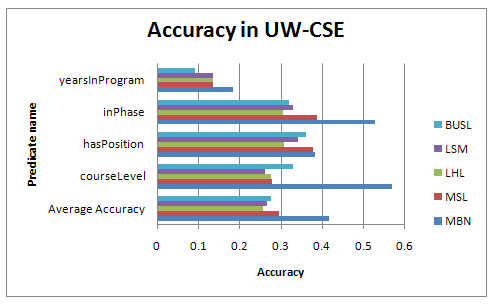
\includegraphics[width=0.7\textwidth]{UWCSE_ACC.png}
}
\caption{Predictive Accuracy by attribute, measured by 5-fold cross-validation. The methods are ordered as shown, with $MBN$ at the bottom. \label{fig:UWCSE_ACC}}
\end{center}
\end{minipage}
\begin{minipage}{0.5\linewidth}
\begin{center}
\resizebox{1\textwidth}{!}{
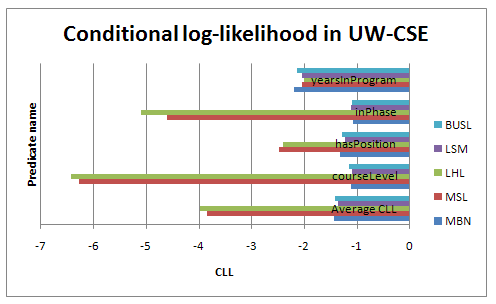
\includegraphics[width=0.4\textwidth]{UWCSE_CLL.png}
}
\caption{Conditional Log-likelihood by attribute, measured by 5-fold cross-validation. The methods are ordered as shown, with $MBN$ at the bottom. \label{fig:UWCSE_CLL}}
\end{center}
\end{minipage}
\end{figure}


% Table generated by Excel2LaTeX from sheet 'Sheet1'
\begin{table}[htbp]
  \centering
  \caption{Cross-validation averages for the UW-CSE dataset}
    \begin{tabular}{|r|r|r|r|r|r|} \hline
          & \textbf{MSL} & \textbf{LHL} & \textbf{LSM} & \textbf{BUSL} & \textbf{MBN} \\\hline
    Time(min) & 2160  & 2413  & 2     & 276   & \textbf{0.6} \\\hline
    Accuracy & 0.29 & 0.25 & 0.26 & 0.27 & \textbf{0.41} \\\hline
    Conditional log-likelihood   & -3.85 & -3.98 & \textbf{-1.37} & -1.42 & -1.43 \\\hline
    \end{tabular}%
  \label{tab:UWCSE}%
\end{table}%




Our results 
%reported in Section~\ref{sec:basic-eval} 
indicate that the two most recent Markov Logic Network structure learning methods----Lifted Hypergraph Learning and Learning Structural Motifs---show the best performance. This is confirmed in independent empirical studies by other researchers \cite{Kok2010}. The remaining sections of the paper therefore focuses on comparing LHL and LSM with the moralization approach.

\subsection{Comparison with Inductive Logic Programming on Mutagenesis}

We compare the performance of the learn-and-join algorithm for a classification task, predicting the mutagenicity of chemical compounds. This problem has been extensively studied in Inductive Logic Programming (ILP). The purpose of this comparison is to benchmark the predictive performance of the moralization approach against discriminative learning by methods that are different from Markov Logic Network learners. 

The class attribute is the mutagenicity (log p). Compunds recorded as having positive mutagenicity are labeled active (positive examples) and compounds recoreded as having 0 or negative mutagenicity are labeled inactive (negative examples). The database contains a total of 188 compounds. Whereas Inductive Logic Programming methods are discriminative, the moralization method performs generative learning over all attributes, a significantly more difficult task. 
We  compare the predictive accuracy of the Moralized Bayes net  with well-known ILP methods. Table \ref{table:muta} presents the results of Lodhi and Muggleton \cite{Lodhi2005}. For the STILL system, we followed the creators' evaluation methodology of using a randomly chosen training and test set. The other systems are evaluated using 10-fold cross-validation. The table shows that the classification performance of the generative Moralized Bayes net model matches that of the discriminative Inductive Logic Programming models.

\begin{table}[h]
\begin{center}
\begin{tabular}{|l|l|l|l|}
\hline
 Method & Evaluation & Accuracy & Reference\\ \hline
MBN &10-fold & 0.87& \\ \hline
P-progol &10-fold & 0.88&\cite{Muggleton1996} \\ \hline
FOIL &10-fold & 0.867& \cite{Quinlan1996}\\ \hline
STILL &90\%train-10\%test & 0.936& \cite{Sebag1997} \\ \hline
MBN &90\%train-10\%test & 0.944& \\ \hline

\end{tabular}
\end{center}

\caption{A comparison of the Moralized Bayes net method with standard Inductive Logic Programming systems trained to predict mutagenicity. Although Bayes net learning produces a generative model, its performance is competitive with discriminative learners.\label{table:muta}}
\end{table}%	


\section{Learning Autocorrelations}

In this section we focus on databases that feature self-relationships between entities of the same type. Such schemas potentially give rise to autocorrelations where the value of an attribute for an entity can be predicted by the value of the same attribute for related entities. While such recursive dependencies are a key statistical phenomenon in relational data, discovering valid autocorrelations has been a challenge for statistical-relational methods \cite{jensen-auto,Neville2007}. We investigate how well our approach using the main functor form discovers autocorrelations compared to general Markov Logic structure learning methods. Our benchmark databases are the synthetic University+ dataset and the real-world Mondial database.
Table~\ref{table:recurse} shows the recursive dependencies discovered by the learn-and-join algorithm on each database. We use clausal notation of the form $\it{child} \leftarrow \{\it{parents}\}$. {\em Neither of the Markov Logic methods LHL nor LSM discovered any recursive dependencies.}

\begin{table}[t]
\begin{center}
\begin{tabular}{|l|l|}
\hline
Database & Recursive Dependency Discovered \\ \hline
University &$gpa(X) \leftarrow  ranking(X), grade(X,Y) , registered(X,Y), friend(X,Z), gpa(Z) $\\ \hline
University &$\it{coffee}(X) \leftarrow coffee(Y), friend(X,Y)$\\ \hline
Mondial &$\it{religion} (X) \leftarrow continent(X) , border(X,Y), \it{religion}(Y)$\\ \hline
Mondial &$continent(X) \leftarrow  border(X,Y), continent(Y), gdp(X) , \it{religion}(Y)$\\ \hline
\end{tabular}
\end{center}
\caption{Autocorrelations discovered by the learn-and-join algorithm using the main functor constraints.\label{table:recurse}}
\end{table}%

Table~\ref{table:university} and \ref{table:mondial} show the runtime and average predictive performance. The time reported for MBN includes both structure and parameter learning. To achieve a high resolution, results on Mondial are based on 5-fold cross validation. The University dataset is small, so we test and train on the same dataset. As in the previous experiments, both MBN and LSM are fast. The predictive accuracy using Markov Logic Network inference was much better in the moralized Bayes net model (average accuracy improved by 25\% or more). This indicates that the discovered recursive dependencies are important for improving predictions.



\begin{table}[t] \centering
\small{
\begin{minipage}{0.5\linewidth}
\begin{tabular}
{|l||l||l||l|}\hline
&MBN  &LSM&LHL\\ \hline
Time (seconds) &12&\textbf{1}&2941\\ \hline
%Number parameters &223&33&52 \\ \hline
Accuracy & \textbf{0.85}&0.44&0.47\\ \hline
CLL &\textbf{-0.8}&-2.21&-4.68\\ \hline
\hline
\end{tabular}
\caption{Results on the University+ database. \label{table:university}} 
\end{minipage}
\begin{minipage}{0.4\linewidth}
%{\small

\begin{tabular}
{|l||l||l||l|}\hline
&MBN  &LSM&LHL\\ \hline
Time (seconds)& 50&\textbf{2}&15323\\ \hline
%Number parameters &242&15 &23 \\ \hline
Accuracy &\textbf{0.50}&0.26&26\\ \hline
CLL &\textbf{-1.05}&-1.43&-3.69\\ \hline
\hline
\end{tabular}
\caption{Results on the Mondial database. \label{table:mondial}} 
\end{minipage}

}
\end{table}
%

 


%\begin{tabular}
%{|l||l||l||l|}\hline
%&MBN  &LSM&LHL\\ \hline
%Time (seconds)& 50&2&15323\\ \hline
%%Number parameters &242&15 &23 \\ \hline
%Accuracy &0.50&0.26&26\\ \hline
%CLL &-1.05&-1.43&-3.69\\ \hline
%\hline
%\end{tabular}
%\caption{Learning Times and Predictive Performance on Databases with Autocorrelations. \label{table:auto-results}} 
%\end{table}

\section{Lesion Studies}
In this section we study the effects of relaxing different constraints used in the learn-and-join algorithm. We focus on the main functor constraint for learning autocorrelations, and on the lattice constraints. The other constraints simply reflect the semantics of the relational schema rather than learning principles. To achieve a high resolution, all results are based on 5-fold cross validation. We report a number of quantities for comparing the learned structures.

\begin{description}
\item[\textbf{SLtime(s)}]  Structure learning time in seconds
\item [\textbf{Numrules}] Number of clauses in the Markov Logic Network excluding rules with weight 0.
% to as a method to compare the quality of structure. 
\item [\textbf{AvgLength}] The average number of atoms per clause.
\item [\textbf{AvgAbWt}] 
%The weight of a clause is an indication of how important a clause is. Since large negative weights for clauses also show a strong correlation we compute 
The average absolute weight value.
\end{description}

Because constraints curtail the search space, we expect constrained methods to have the following effects compared with unconstrained methods.

\begin{enumerate}
\item Faster run-time. 
\item A simpler model with fewer rules.
\item If the constraints are chosen well, they should allow the system to identify important rules and not impair predictive performance.
\end{enumerate}
 

\subsection{Main Functor Constraints}
We remove the constraints of specifying a main functor node to study its importance. This means that we introduce a copy of an entity table that is potentially involved in an autocorrelation (e.g., in the University+ database, there are two tables $\it{Student}_{1}, \it{Student}_{2}$). This duplication approach is used other relational learning systems (e.g., \cite{Yin2004,Yin2008a}). 
The unconstrained method applies the learn-and-join algorithm in the same way to all entity tables, including the copies.
We investigated the following main hypotheses about the effect of the main functor constraint.

\begin{enumerate}
		\item There should be a tendency towards longer clauses associated with the main functor node (see Section \ref{sec:main-node}).
	\item Since Proposition \ref{prop:normal} implies that the ground models with and without the constraint are the same, predictive accuracy should be similar.
	\item The duplicate edges should lead to duplicate clauses without improvement in predictive performance since the ground models are the same.
	\end{enumerate}

Table \ref{tab:MainFuncUniversity} shows the results for University and Table \ref{tab:MainFuncMondial} shows the results for Mondial dataset. {\em Constraint} is the learn-and-join algorithm with the main functor constraint, whereas {\em Duplicate} is the learn-and-join algorithm applied naively to the duplicate tables without the constraint.
As expected, the constraint speeds up structure learning, appreciably in the case of the larger Mondial dataset. The number of clauses is significantly less (50-60), while on average clauses are longer.  The size of the weights indicates that the main functor constraint focuses the algorithm on the important rules.

% The predictive accuracy measurements are very similar, in fact the averages over all 5-folds are identical. The recursive dependencies discovered were the same.


 
% Table generated by Excel2LaTeX from sheet 'Sheet1'
\begin{table}[htbp]
%\begin{minipage} {0.5\linewidth}
% \resizebox{0.4 \textwidth}{!}{
  \centering
      \begin{tabular}{|l|l|l|}

  \hline
           & Constraint & Duplicate \\ \hline
 
    SLtime(s) & \textbf{3.1} & 3.2 \\ \hline
    \# Rules & \textbf{289} & 350 \\\hline
    AvgLength & 4.26 & 4.11 \\\hline
    AvgAbWt & \textbf{2.08} & 1.86 \\\hline
    ACC & \textbf{0.86} & \textbf{0.86} \\\hline
    CLL & \textbf{-0.89} & \textbf{-0.89} \\\hline
 
    \end{tabular}%
 %}
  \caption{Comparison to study the effects of removing Main Functor Constraints on University+ dataset.  \label{tab:MainFuncUniversity}}%
 %\end{minipage}
\end{table}%


% Table generated by Excel2LaTeX from sheet 'Sheet1'
%\begin{minipage} {0.5\linewidth}
\begin{table}[htbp]
  \centering
    \begin{tabular}{|r|r|r|}     \hline
           & Constraint & Duplicate \\\hline
     SLtime(s) & \textbf{8.9} & 13.1 \\\hline
   \# Rules & \textbf{739} & 798 \\\hline
    AvgLength & 3.98 & 3.8 \\\hline
    AvgAbWt & 0.22  & \textbf{0.23} \\\hline
    ACC & \textbf{0.43} & \textbf{0.43} \\\hline
    CLL & \textbf{-1.39} & \textbf{-1.39} \\ \hline
 
    \end{tabular}%
   \caption{Comparison to study the effects of removing Main Functor Constraints on Mondial dataset.\label{tab:MainFuncMondial}}
% \end{minipage}
\end{table}%


We also report the number of clauses of a given chain length. Since a clause contains conditions on both attributes and links, we use the maximal slot chain length: The chain length of a rule is computed as the maximal length of a sequence of predicates appearing in the rule such that the database tables corresponding to the predicates are related by foreign key pointers \cite{Getoor2007c}. The measurements show that potentially the algorithm can find long chains, although informative long chains are rare.
% we just compute this as the number of variables per rule. Can be long if we put together two short chains, e.g. student intelligence is predicted by course difficulty and by professor popularity

%TODO: would be nice to show actual Mondial graph with duplicate edges.

\begin{figure*}[htbp] %  figure placement: here, top, bottom, or page
   \centering
   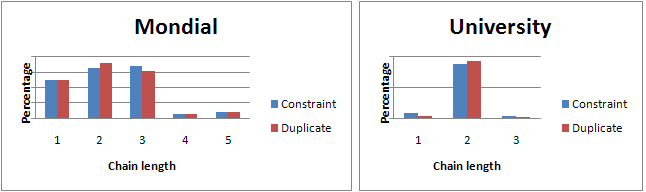
\includegraphics[width=4in]{chain_length2.png}
   \caption{The figure illustrates the  percentage of rules of a given chain length for Mondial and University+ dataset in the autocorrrelation lesion study.}
\label{fig:chainlength2}
\end{figure*}
 
\subsection{Lattice Constraints}

A key feature of the learn-and-join algorithm is the use of lattice constraints. In terms of the join lattice, Bayes nets for join tables higher in the lattice inherit the edges from Bayes nets for join tables lower in the lattice. 
We remove this constraint to assess its effect on learning. If the Bayes nets learned for different join tables are no longer constrained to be consistent with each other, the question arises how to merge them into a single Bayes net. One possibility is to learn a Bayes net for the maximum join table (e.g., for the relationship set $\it{Registered}(\S,\C),\it{Teaches}(\P,\C)$ in Figure~\ref{fig:university-tables}). However, in experiments we found that for our benchmark datasets, the maximum join table is too small to yield meaningful results, because too few tuples meet the join conditions (e.g., not many students are RAs). We therefore investigated an intermediate approach where different Bayes nets are learned for single relationship tables joined with the associated entity tables (e.g., $\it{Registered(\S,\C)} \Join \it{Student} \Join \it{Course}$). In our benchmark datasets, there were very few conflicts between the edges in different Bayes nets, which we broke randomly. So we could obtain a single acyclic graph for the database by merging the graphs of the intermediate joins; we refer to this approach as the {\em intermediate} method.

%We investigated the following hypotheses.
%
%\begin{enumerate}
%\item The analysis of Section ?? suggests that the lattice constraints should lead to faster run-time. 
%%This effect should be more pronounced as the size of the join tables increases.
%\item The constraints eliminate possible clauses from the search space and give higher priority to clauses that involve shorter slot chains. They should therefore lead to a simpler model with fewer rules.
%\end{enumerate}

Tables \ref{tab:LatticeUniversity}, \ref{tab:LatticeHepatitis}, and \ref{tab:LatticeMondial}  shows the results for the University+, Hepatitis, and Mondial datasets. The numbers are averages from 5-fold cross validation. Folds are formed by randomly selecting entities as described in Section~\ref{sec:datasets}. The lattice constraints speed up the learning time spent on join tables, which is the dominant factor. The constrained model features fewer rules with comparatively higher weights. The average predictive accuracy was somewhat higher than with the unconstrained model, whereas the conditional log-likelihood performance was very similar. This is evidence that the constraints helped identify predictively relevant clauses.
% Table generated by Excel2LaTeX from sheet 'Sheet1'
\begin{table}[htbp]
  \centering
      \begin{tabular}{|r|r|r|} \hline
    & Constraint & Intermediate \\\hline
    SLtime(s) & \textbf{3.1} & 3.3 \\\hline
    \# Rules & \textbf{289} & 443 \\\hline
    AvgAbWt & \textbf{2.08} & 1.86 \\\hline
    AvgLength & 4.26  & 4.94 \\\hline
    ACC & \textbf{0.86} & 0.84 \\\hline
    CLL & \textbf{-0.89} & -0.9 \\\hline
    \end{tabular}%
  \caption{Comparison to study the effects of removing Lattice Constraints on the University+ dataset.\label{tab:LatticeUniversity}}
\end{table}%


% Table generated by Excel2LaTeX from sheet 'Sheet1'
\begin{table}[htbp]
  \centering
  
    \begin{tabular}{|r|r|r|} \hline
          & Constraint & Intermediate \\\hline
    SLtime(s) & \textbf{5.2} & 6.1 \\\hline
   \# Rules & \textbf{818} & 848 \\\hline
    AvgAbWt & \textbf{1.68} & 1.53 \\\hline
    AvgLength & 4.15  & 4.11 \\\hline
    ACC & \textbf{0.47} & 0.41 \\\hline
    CLL & \textbf{-1.31} & -1.34 \\\hline
          
    \end{tabular}%
  \caption{Comparison to study the effects of removing Lattice Constraints on the Hepatitis dataset.\label{tab:LatticeHepatitis}}%
\end{table}%

%\marginpar{Why Hepatitis?}

% Table generated by Excel2LaTeX from sheet 'Sheet1'
\begin{table}[htbp]
  \centering

    \begin{tabular}{|r|r|r|} \hline
          & Constraint & Intermediate \\\hline
    SLtime(s) & \textbf{8.9} & 13.2 \\\hline
    \# Rules & \textbf{739} & 1053 \\\hline
    AvgAbWt & \textbf{0.22} & 0.24 \\\hline
    AvgLength & 3.98  & 4.66 \\\hline
    ACC & \textbf{0.43} & 0.37 \\\hline
    CLL & \textbf{-1.39} & \textbf{-1.39} \\\hline
    \end{tabular}%
   \caption{Comparison to study the effects of removing Lattice Constraints on Mondial dataset \label{tab:LatticeMondial}}
\end{table}%

\begin{figure*}[htbp] %  figure placement: here, top, bottom, or page
   \centering
   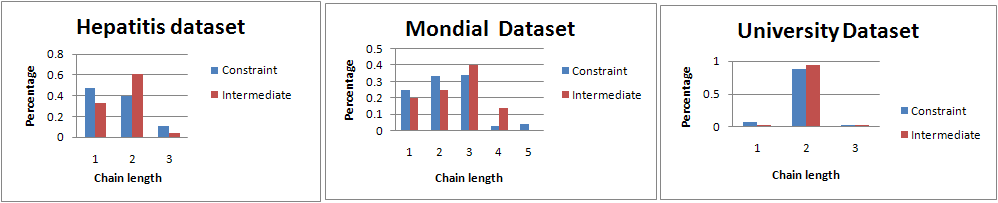
\includegraphics[width=5in]{chain_length1.png}
   \caption{The figure illustrates the  percentage of rules of a given chain length for Hepatitis, Mondial, and University dataset in the Lattice constraint lesion study.}
\label{fig:chainlength1}
\end{figure*}

\section{Conclusion and Future Work} %

This paper considered the task of building a statistical-relational model for databases with many descriptive attributes. We combined Bayes net learning, one of the most successful machine learning techniques, with Markov Logic networks, one of the most successful statistical-relational formalisms. The main algorithmic contribution is an efficient new structure learning algorithm for a parametrized Bayes net that models the joint frequency distribution over attributes in the database, given the links between entities. Moralizing the BN leads to an Markov Logic Network structure. Our evaluation on six benchmark databases with descriptive attributes shows that compared to current Markov Logic Network structure learning methods, the approach using moralization improves the scalability and run-time performance by orders of magnitude. With standard parameter estimation algorithms and prediction metrics, the moralized Markov Logic Network structures make substantially more accurate predictions.
%
We discuss limitations of our current system and how they may be addressed in future work.

{\em Parameter Estimation.} In this work we used generic Markov Logic Network algorithms for parameter estimation implemented in the Alchemy package. While the parameter estimation routines of Alchemy run much faster than the structure learning routines, on some datasets we found that parameter estimation can still take a long time. As Markov Logic Networks obtained by moralization have a special structure, it may be possible to design fast parameter estimation routines for them.

%{\em Pruning and Local Independencies.}
%A disadvantage of learning at the predicate level rather than the literal level is that the resulting Markov Logic Networks contain a relatively large number of formulas; basically, each CP-table row in the parametrized Bayes net becomes a formula in the moralized Bayes net. Often there are local independencies that  allow CP tables to be represented more compactly. SRL research has used decision trees as an effective compact representation for CP-tables \cite{Getoor2001}. This suggests that combining decision trees with parametrized Bayes nets will lead to more parsimonious Markov Logic Network structures. Another possibility is to use Markov Logic Network weight estimation procedures to prune uninformative clauses.
%%We observed that the Alchemy routines assign 0 weight to some uninformative clauses;
%Huynh and Mooney \cite{Huynh2008} show that L1-regularization can be an effective method for pruning a large set of Markov Logic Network clauses.

{\em Link Prediction.} The learn-and-join algorithm learns a model of the distribution over descriptive attributes conditional on the relationship information in the database. An important project is to extend the learn-and-join algorithm so that it can learn not only dependencies among attributes, but also among relationships (e.g. $\it{Daughter}(\X,\Y)$ implies $\it{Parent}(\X,\Y)$). Since previous Markov Logic Network algorithms have performed well in link modelling, an interesting approach would be a hybrid system that uses the output of the learn-and-join algorithm as a starting point for an Alchemy-based structure learning system. In principle, the key ideas of the learn-and-join algorithm such as the lattice and main functor node constraints should also be applicable to link prediction problems.

%\section*{Acknowledgements}

\begin{acknowledgements}
This research was supported by a Discovery Grant from the Natural Sciences and Engineering Council of Canada (NSERC). Preliminary results were presented at the 2010 AAAI conference, the 2011 ILP conference, to the AI group at the University of British Columbia, and the IJCAI-STRUCK and IJCAI-GKR workshops (2009). We are grateful to the audiences for helpful questions and comments, especially Lise Getoor.
\end{acknowledgements}

\bibliographystyle{plain}
\bibliography{master}
\end{document}

\section{INTRO FOR LILNK PREDICTION}


Khosravi {\em et al.} provide a detailed discussion of the differences between the moralization approach and other MLN learning methods \cite{Khosravi2010}. The main differences are as follows. (1) The learn-and-join algorithm uses BN learning, whereas most other MLN methods use techniques from Inductive Logic Programming (ILP). (2) The learn-and-join algorithm learns associations at the level of predicates (attributes and relationships), rather than clauses.

\section{Introduction} [special case of theta-subsumption lattice. Constraints express structural knowledge.] The field of statistical-relational learning (SRL) has developed a number of new statistical models for relational databases \cite{SRL2007}. Markov Logic Networks (MLNs) form one of the most prominent SRL model classes; they generalize both first-order logic and Markov network models \cite{Domingos2007}. MLNs have achieved impressive performance on a variety of SRL tasks. Because they are based on undirected graphical models, they avoid the difficulties with cycles that arise in directed SRL models \cite{bib:jensen-chapter,Domingos2007,Taskar2002}.
%\cite{Domingos2007,Taskar2002}.
An open-source benchmark system for MLNs is the Alchemy package \cite{Kok2009a}.

\paragraph{The Moralization Approach to MLN structure learning}

One of the most effective MLN structure learning methods is the moralization
approach:
First, learn a parametrized Bayes net (FBN) \cite{Poole2003} for relational data. Second, convert the BN to an MLN via moralization (connect spouses and omit edge directions). This approach combines the efficiency and reliability of BN learning with the conceptual advantages and inference capabilities of MLNs. Khosravi {\em et al.} developed the learn-and-join algorithm (LAJ) for BN structure learning from relational data \cite{Khosravi2010}. The algorithm upgrades a single-table BN learner: it constructs larger and larger table joins that are presented as data tables to the BN learner. The results of learning on smaller joins are propagated as edge constraints to learning on larger joins. Khosravi {\em et al.} show theoretically that although larger joins imply more BN  nodes, the edge constraints keep the model search space essentially the same size. In empirical evaluation, the LAJ algorithm improves runtimes by a factor of 200-1,000 compared to previous MLN learning systems. Predictive accuracy also improves substantially by several measures.

The LAJ algorithm constructs join data tables that are joins of relationship tables. This means that the learner searches for correlations among attributes {\em conditional on} the existence of a relationship. Thus the learner does not search for correlations between relationships. Intuitive examples of such correlations would be ``if $\X$ is friends with $\Y$, then $\X$ is more likely to send $\Y$ a message'', or ``if $\X$ is friends with $\Y$, and $\Y$ is friends with $\Z$, then $\X$ is more likely to be friends with $\Z$''. In this paper we extend the LAJ algorithm to learn correlations among relationships. The main challenge in the extension is that it is computationally infeasible to compute a data table that enumerates entities that are {\em not} related, because there are too many. Instead of a data table, we compute a {\em frequency table} that lists the frequencies with which combinations of joint value assignments to the Bayes net nodes occur in the database. We utilize a virtual join algorithm that efficiently computes these frequencies, including frequencies that involve nonexistent relationships, {\em without} enumerating the set of unrelated pairs of tuples. Essentially the virtual join algorithm is a dynamic program for computing the Moebius parameters of a set of binary random variables [cite nips, sdm paper]. We modify the single-table BN learner so that it takes as input a frequency table rather than a data table. This is straightforward as BN learners usually use the data table only to compute frequencies (sufficient statistics).

%To facilitate the more complex model search, we organize the search results according to the levels in the subset lattice whose points are sets of relationship tables. Level-wise lattice search is a well-known search design, familiar from the Apriori algorithm, that provides conceptual clarity and computational efficiency.

For empirical evaluation, we apply the lattice search to four relational databases. The benchmark runtimes of the algorithm are excellent, with structure learning times ranging from 1 to 10 minutes. The extended LAJ algorithm discovers a number of adjacencies between relationship indicator nodes, which substantially improve the prediction of both relationships and attributes.

\section{Link Prediction Models}

In this section we consider learning dependencies involving relationships, rather than dependencies between attributes given relationships. Graphically, this amounts to learning edges that point to relationship nodes.
%Our approach is to learn a model of the joint distribution among relationship nodes, rather than a set of models for different relational contexts.
The main challenge in applying Bayes net learning is computational: A link prediction model needs to consider empirical statistics that involve {\em nonexistent} or absent links. A naive approach to computing such sufficient statistics would be to construct a data table by enumerating unrelated tuples of objects. A numerical example will illustrate why this is infeasible. Consider a university database with 20,000 Students, 1,000 Courses and 2,000 TAs. If each student is registered in 10 courses, the size of the $\it{Registered}$ table is $200,000 = 2 \times 10^{5}$. So the number of complementary student-course pairs is $2 \times 10^{7}-2 \times 10^{5}$, which is a much larger number that is too big for most database systems. If we consider joins, complemented tables are even more difficult to deal with: suppose that each course has at most 3 TAs. Then the number of satisfying instantiations of $\it{Registered}(\S,\course),\it{TA}(\T,\course)) < 6  \times 10^{5}$, whereas for $\neg \it{Registered}(\S,\course),\neg \it{TA}(\T,\course))$ that number is on the order of $4 \times 10^{10}$.

\subsection{The Frequency Table and Model Score Comparison}
Getoor {\em et al.} observed that in the case of a single relationship functor $\Relation(\X,\Y)$, sufficient statistics can be obtained without enumerating all pairs in the relation complement, by using a ``1-minus'' trick: The database frequency of a condition involving the negation $\Relation(\X,\Y) = \false$ is 1 minus the frequency of the condition with $\Relation(\X,\Y) = \true$. It is possible to extend this insight to develop an efficient dynamic programming algorithm for the case of multiple relations that {\em does not enumerate tuples that fail to satisfy a relationship.} The next section provides the details of this algorithm; here we show it can be applied to upgrade a single-table BN learner for multi-relational learning.

Let $\F = \functor_{1}(\term_{1}),\ldots,\functor_{k}(\term_{k})$ be a finite set of functors. A \textbf{frequency table} for $\F$ and database $\D$ is a table $\ftable(\F,\D)$ with $k+1$-columns such that for each possible joint assignment $\functor_{1}(\term_{1}) = \a_{1},\ldots,\functor_{k}(\term_{k}) = \a_{k}$, there is exactly one row in $\ftable(\F,\D)$. The $k+1$-st column specifies the database frequency $P_{\D}(\functor_{1}(\term_{1}) = \a_{1},\ldots,\functor_{k}(\term_{k}) = \a_{k})$.

{\em Example.}

\paragraph{Model Selection Score Comparison}

A single-table model selection score has the form $\score(\G,\datatable)$ where $\G$ is a graphical model and $\datatable$ a data table. We consider scores that trade off data fit against model complexity, and that can be computed given the following quantities.

\begin{enumerate}
 % \item The log-likelihood $L_{\G}(\datatable)$.
  \item The sufficient data statistics for joint functor value assignments.
  %events $\p_{ijk}(\datatable)$.
  \item The number of parameters $\parameters_{\G}$.
  \item The sample size $m = $ number of rows in $\datatable$.
\end{enumerate}

We also assume that the score is {\em decomposable}, i.e. can be written as the sum of local scores for each node in the BN.
An example is the Bayes Information Criterion (BIC) score \cite[Ch.8.3.2]{Neapolitan2004}
\[
\mathit{BIC}(\G,\datatable) \equiv ln(P_{\widehat{G}}(\datatable)) - \parameters(\G) \cdot \frac{ln(m)}{2}
\]
where $\widehat{G}$ is the BN $\G$ with its parameters instantiated to be the maximum likelihood estimates given the datatable $\datatable$, and $\parameters(\G)$ is the number of free parameters in the structure $\G$.


In the relational context, we use a frequency table that lists the database frequencies of each joint assignment to a given set of functors (typically, joint assignments to a node and its parents). For the sample size, we use the number of all possible groundings of the variables in the functors. Knowing this number allows an algorithm to convert database frequencies to counts if necessary. Algorithm~\ref{alg:compare} shows pseudocode for the comparison procedure.

\begin{algorithm}[htb]
\linesnumbered
\SetKwData{Calls}{Calls}
\SetKwData{Notation}{Notation}
%\begin{algorithmic}
%{\footnotesize
%\STATE {\em Input}: Database $\D$ with $\etable_1,..\etable_e$ entity tables, functors $\F$, variable number bound $\varbound$.
\KwIn{Database $\D$; Join Bayes nets $\B^{*},\B$.}
\KwOut{Difference in model selection score $\score(\B,\D) - \score(\B^{*},\D)$.}
\begin{algorithmic}
\STATE \Calls $\lscore(\functor_{i},\B^{*},\B,\ftable,m)$: procedure that computes the local model selection score difference for functor node $\functor_{i}$ between a current graph $\B$ and a candidate graph $\B^{*}$ given database $\D$.
\STATE \Calls $\ftable(\F,\D)$: procedure that constructs a table that lists the frequencies of joint assignments to functors $\F$ in database $\D$.
\STATE \Notation $|\population_{\X}|$: the size of the population associated with population variable $\X$ in database $\D$.
%\STATE \Notation: $\it{BNL}(\ftable,\it{Econstraints},m)$ is the output DAG of the BN learner given frequency table $\ftable$, constraints $\it{Econstraints}$, and base size $m$.
%. Get-Constraints$(\G)$ specifies a new set of edge constraints, namely that all edges in $\G$ are required, and edges missing between variables in $\G$ are forbidden.
%} %fnsize
\end{algorithmic}
\begin{algorithmic}[1]
\STATE $\lscore := 0$.
\FORALL{functor nodes $i$ such that $\parents_{i,\B^{*}} \neq \parents_{i,\B}$}
\STATE $\F_{i} := \functor_{i} \cup \parents_{i,\B^{*}} \cup \parents_{i,\B}$.
\STATE $\ftable_{i} := \ftable(\F_{i},\D)$.
\STATE $m_{i} := \prod_{\X} |\population_{\X}|$, where $\X$ is a population variable appearing in $\F_{i}$.
\STATE $\lscore += \lscore(\functor_{i},\B^{*},\B,\ftable_{i},m_{i})$.
\ENDFOR
\RETURN $\lscore$.	
\end{algorithmic}
%\label{alg:cpt}
\caption{Pseudocode for model selection comparison of two Join Bayes Nets \label{alg:compare}}
\end{algorithm}

\subsection{Structure Learning for Link Prediction}

Given the procedure for numerically comparing different candidate models, it is straightforward to incorporate relational constraints. Algorithm~\ref{alg:2R} presents pseudocode for a simple hill-climbing search. The algorithm can be adapted easily for more complex search strategies. In our experiments, we used the GES method. Table~\ref{table:2R} specifies the constraints for learning edges that point into relationship indicators. The main impact of first running an algorithm for learning A2A edges is to introduce cyclicity constraints. For instance, if the A2A algorithm introduces an edge of the form $\R(\X,\Y) \rightarrow \functor(\X)$, then the 2R algorithm rules out the edge $\R(\X,\Y) \leftarrow \functor(\X)$.

\begin{algorithm}[htb]
\linesnumbered
\SetKwData{Calls}{Calls}
\SetKwData{Notation}{Notation}
%\begin{algorithmic}
%{\footnotesize
%\STATE {\em Input}: Database $\D$ with $\etable_1,..\etable_e$ entity tables, functors $\F$, variable number bound $\varbound$.
\KwIn{Database $\D$; functors $\F$; \#variable bound $\varbound$.}
\KwOut{MLN formulas for $\D,\F$; a Join Bayes net with relationship functors as children.}
\begin{algorithmic}
\STATE \Calls $\it{Compute\_Score}(\B,\B^{*},\D)$: procedure that computes the model selection score difference between a current graph $\B$ and a candidate graph $\B^{*}$ given database $\D$.
%\STATE \Notation: $\it{BNL}(\ftable,\it{Econstraints},m)$ is the output DAG of the BN learner given frequency table $\ftable$, constraints $\it{Econstraints}$, and base size $m$.
%. Get-Constraints$(\G)$ specifies a new set of edge constraints, namely that all edges in $\G$ are required, and edges missing between variables in $\G$ are forbidden.
%} %fnsize
\end{algorithmic}
\begin{algorithmic}[1]
%{\footnotesize
%	\STATE Add descriptive attributes of all entity and relationship tables as variables to  $G$. Add a boolean indicator for each relationship table to $G$.
	\STATE Econstraints := Relational Redge Constraints from Table~\ref{table:redge}.
	\STATE Econstraints := Apply LAJ algorithm~\ref{alg:struct} to learn attribute-attribute edges.
	\STATE Constraints := Econstraints +  for each functor node, the number of first-order variables in its family is no greater than $\varbound$.
	\COMMENT{Apply local BN search method with constraints.}
	\STATE Initialize local search.
	\REPEAT
	\STATE Let $\B^{*}$ be current graph.
	\FORALL{Candidate Graphs $\B$ satisfying Constraints}
	\STATE $\score(\B) := \it{Compute\_Score}(\B,\B^{*},\D).$
	\IF{there is higher-scoring candidate graph}
	\STATE $\B^{*} :=$ highest-scoring candidate graph.
	\ENDIF
	\ENDFOR
	\UNTIL{No candidate graph scores higher.}
	\RETURN $\B^{*}$.	
\end{algorithmic}
%\label{alg:cpt}
\caption{Pseudocode for MBN structure learning for link prediction \label{alg:redge}}
\end{algorithm}


\begin{table} \caption{Constraints for learning link prediction edges that point towards relationship indicator nodes. For a functor node $\functor(\terms)$, the \textbf{family} of $\functor(\terms)$ is $\functor(\terms)$ together with its parents.
 %$\set{\Relation}_{\functor(\terms)}$ comprise the set of relationship nodes that occur in the family of $\functor(\terms)$.
%%The notation $\B_{\etable}$  denotes the BN associated with entity table $\etable$, the notation $\B_{\set{\Relation}}$ the BN associated with relationship set $\set{\Relation}$.
\label{table:redge}}
For each functor node $\functor(\terms)$, the  following must hold.
\begin{enumerate}
\item Forbidden Edges: If $\B$ contains $\functor(\terms) \rightarrow \functor'(\terms')$, then $\functor'(\terms')$ is the main functor for $\functor'$ and $\functor$ or $\functor'$ is a predicate $\Relation$. \label{clause:redge}
\item Family Connections: For each functor node $\functor(\terms)$, the family of $\functor(\terms)$ is connected. That is, there is an ordering $\functor_1(\terms_1),\ldots,\functor_k(\terms_k)$ of the family nodes such that for each $i<k$, the nodes $\functor_i(\terms_i)$ and $\functor_{i+1}(\terms_{i+1})$ share at least one first-order variable.
     \label{clause:chain}
%\item % Family II: For each functor node $\functor(\terms)$, if $\functor'(\terms')$ is an attribute node that occurs in the family of $\functor(\terms)$, then $\functor'(\terms')$ shares at least one population variable with at least  one relationship node in $\set{\Relation}_{\functor(\terms)}$. \label{clause:chain2}
\end{enumerate}
\end{table}

\section{Edge Constraints}

We now discuss the motivations for the constraints of Table~\ref{table:redge}. Constraint~\ref{clause:chain} is based on the fact that

%\begin{table} \caption{Relationship edge constraints for learning link prediction edges that point towards relationship indicator nodes. For a relationship functor $\Relation(\X,\Y)$, let $\set{\Relation}_{\Relation(\X,\Y)}$ comprise $\Relation(\X,\Y)$ plus the set of relationship nodes that occur among the parents of $\Relation(\X,\Y)$.
%%The notation $\B_{\etable}$  denotes the BN associated with entity table $\etable$, the notation $\B_{\set{\Relation}}$ the BN associated with relationship set $\set{\Relation}$.
%\label{table:2R}}
%\begin{enumerate}
%\item Forbidden Edges: If $\B$ contains $\functor(\terms) \rightarrow \functor'(\terms')$, then $\functor'(\terms')$ is the head functor for $\functor$ and $\functor$ or $\functor'$ is a predicate $\Relation$. \label{clause:redge}
%\item Family I: The set $\set{\Relation}_{\Relation(\X,\Y)}$ is connected.
%\item  Family II: If $\functor$ is an attribute node that occurs among the parents of $\Relation(\X,\Y)$, then $\functor$ shares at least one population variable with at least  one relationship node in $\set{\Relation}_{\Relation(\X,\Y)}$.
%\end{enumerate}
%\end{table}

\subsection{The Virtual Join Algorithm for Computing Database Frequencies}
Joint probabilities involving negated relationship variables can be derived using the {\em M\"obius parametrization} \cite{Drton08}. Given a finite set of binary variables $\X_{1},\ldots,\X_{n}$, the M\"obius parameters are the marginal probabilities of the form $P(\set{X}= 1)$ that assigns 1 to all variables in each subset $\set{X}$ of variables. In the relational setting, if we have three relationship indicator variables $\R_{1},\R_{2},\R_{3}$, the M\"obius parameters are the joint probabilities $P(\R_{i}), P(\R{i},\R_{j}), P(\R_{1},\R_{2},\R_{3})$, for $i,j=1,2,3, i \neq j$. The M\"obius inversion theorem shows that every joint probability involving any number of positive and negative relationship variables, can be computed as an alternating sum of the M\"obius parameters.

To fill in CP-table entries, we need to compute every joint probability, so instead of using the M\"obius formula directly, we utilize an efficient dynamic programming scheme that reuses intermediate results as much as possible. (1) We compute all frequencies that are defined by the same join table at once when the join has been built. (2) We use a JP-table as our data structure for storing the results of intermediate computations (marginal joint probabilities). A JP-table is just like a CP-table whose rows correspond to joint probabilities rather than conditional probabilities. The marginal probabilities are represented with a third value $*$ for relationship predicates (in addition to $\true,\false$). This is used to represent the frequencies where a relationship predicate is unspecified. After initializing the table with the M\"obius parameters, we perform a dynamic-program style update of joint probabilities that involve $k+1$ negative relationships, given that all joint probabilities involving at most $k$ negative relationships have been computed:

\begin{eqnarray}
P(\C, \neg \R) := P(\C) - P(\C, \R).	
	\label{eq:dynamic}
\end{eqnarray}

where $\C$ is a conjunction of atoms involving at most $k$ negative relationship indicators and $\R$ is a relationship predicate. We refer to this dynamic program as the Virtual Join algorithm. Algorithm~\ref{alg:adapted} shows the pseudocode for the VJ algorithm. Figure \ref{fig:example} illustrates the recursion.

\begin{figure*}[htbp] %  figure placement: here, top, bottom, or page
   \centering
   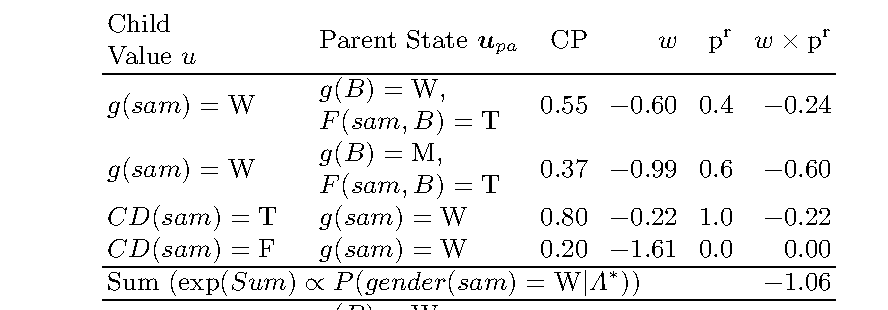
\includegraphics[width=6in]{example.pdf}
   \caption{A frequency with %two
   negated relationships (nonexistent links) can be computed from frequencies that involve positive relationships (existing links) only. The leaves in the computation tree involves existing database tables only. The subtractions involve looking up results of previous computations. % (line 16).
To reduce clutter, we abbreviated some of the predicates.}
\label{fig:example}
\end{figure*}

\begin{algorithm}
\begin{algorithmic}
\STATE \underline{Notation}: A row $\r$ corresponds to a partial or complete assignment for function terms. The value assigned to function term $\f(\set{\theta})$ in row $\r$ is denoted by $\f_{\r}$. The probability for row $\r$ stored in JP-table $\tau$ is denoted by $\tau(\r)$.
\STATE \underline{Input}: database $\D$; child variable and parent variables divided into a set $\set{\R_{1},\ldots,\R_{m}}$ of relationship predicates and a set $\set{C}$ of function terms that are not relationship predicates.
 \STATE \underline{Calls}: initialization function $\join(\set{\C},\true = \R_1 = \cdots = \R_k)$. Computes join frequencies conditional on relationships $\R_{1},\ldots,\R_{k}$ being true.
\STATE \underline{Output}: Joint Probability table $\tau$ such that the entry $\tau(\r)$ for row $\r \equiv
(\set{\C} = \set{\C}_{\r}, \set{\R} = \set{\R}_{\r})$ is the frequencies $P_{\D}(\set{\C} = \set{\C}_{\r}, \set{\R} = \set{\R}_{\r})$ in the database distribution $\D$.
\end{algorithmic}
\begin{algorithmic}[1]

\STATE \COMMENT{fill in rows with no false relationships using table joins}\label{line:start-join}
\FORALL{valid rows $r$ with no assignments of $\false$ to relationship predicates}
\FOR{$i=0$ to $m$}
\IF[$r$ has $m-i$ unspecified relationships]{$r$ has exactly $i$ true relationships$\R^1,..,\R^i$}
\STATE find $P_{\D}(\set{\C} =\set{\C}_{\r}, \set{\R} = \set{\R}_{\r})$ using $\join(\set{\C} =\set{\C}_{\r}, \set{\R} = \set{\R}_{\r})$. Store the result in $\tau(\r)$. \label{line:join}
\ENDIF
\ENDFOR
\ENDFOR \label{line:end-join}

\STATE \COMMENT{Recursively extend the table to JP-table entries with false relationships.}
\FORALL{%valid
rows $r$ with at least one assignment of $\false$ to a relationship predicate}
\FOR{$i=1$ to $m-1$}
\IF[find conditional probabilities when $\R^1$ is true and when unspecified]
{$r$ has exactly $i$ false relationships $\R^1,..,\R^i$}
\STATE Let $\r_{\true}$ be the
row such that (1) $\R^1_{\r_{\true}} = \true$, (2) $\f^{R^1}_{\r_{\true}}$ is unspecified for all attributes $\f^{R^1}$ of $\R^1$, and (3) $\r_{\true}$ matches $\r$ on all other variables.
\STATE Let $\r_{*}$ be the %consistent
row that matches $\r$ on all variables $\f$ that are not $\R^1$ or an attribute of $\R^1$ and has $\R^1_{\r_{*}}$ unspecified.
\STATE \COMMENT{The rows $r_{*}$ and $\r_{\true}$ have one less false relationship variable than $\r$.}
\STATE Set $\tau(\r) := \tau(\r_{*}) - \tau(r_{\true}).$ \label{line:update}
\ENDIF
\ENDFOR
\ENDFOR
\end{algorithmic}
 \caption{The Virtual Join dynamic program for parameter estimation in a Join Bayes Net.\label{alg:adapted}}
\end{algorithm}

%\section{Attribute Prediction with Link Uncertainty: Learning R2A Dependencies}

%The only class of edges in an Bayes net that has not been considered so far are edges of the R2A type, of the form $\Relation(\X,\Y) \rightarrow \f(\X)$, where $\f$ is a unary attribute.
% Abstract for Learning Markov Logic Networks with Link Uncertainty
\begin{abstract} Many machine learning applications that involve relational databases incorporate first-order logic and probability. Markov Logic Networks (MLNs) are a prominent statistical relational model that consist of weighted first order clauses. One of the most effective methods for learning MLN structure is the moralization approach: First learn a parametrized Bayes net (PBN) \cite{Poole2003}, then convert the PBN to an MLN via the standard moralization procedure for converting directed models to undirected models. The learn-and-join algorithm is the most recent moralization algorithm. However, it is currently restricted to learning dependencies among attributes {\em given} the link structure; it does not learn association between links. In this paper we generalize the learn-and-join algorithm to learn an MLN model of the joint distribution over links and attributes. Two algorithmic innovations make this computationally feasible. (1) We design the model search as a level-wise search through a lattice of table sets. The results of learning on smaller lattices are propagated to larger lattices as constraints. (2) We use a virtual join algorithm to compute a summary of sufficient statistics that involve missing links. Empirical evaluation on x benchmark databases shows that the lattice search is fast, and  finds significant dependencies missed by the simple learn-and-join algorithm that lead to better predictions for both links and attributes.
\end{abstract}


\section{OLD STUFF Introduction} This is old writing. The {\em cyclicity problem} arises because the ground BN may contain cycles even when the population model does not. In this case it is not clear how to measure the fit of the model to the data with a likelihood function. A common approach to computational and/or conceptual difficulties in defining a likelihood function is to employ a pseudo-likelihood [cite]; a prominent example in statistical-relational learning (SRL) is the pseudo likelihood defined for Markov Logic Networks (MLNs).


In the single-table learning setting, the goal is often to represent predictive dependencies between the attributes of a single individual (e.g., between the intelligence and ranking of a student). In the SRL setting, the goal is often to represent in addition dependencies between attributes of different individuals that are related or linked to each other (e.g., between the intelligence of a student and the difficulty of a course given that the student is registered in the course). In this paper we apply Bayes nets (BNs) to represent such dependencies. Bayes nets  have been one of the most widely studied and applied generative model classes. A common approach to defining a graphical model for relational data is {\em knowledge-based model construction} (KBMC), which distinguishes two levels of models [cite Koller, Jensen], a 1st-order template or class dependency level model, and an instance-level model (also called the ground or unrolled model) \cite{Getoor2007c,deraedt2007} [poole]. A class-level model $M$ is  instantiated with the specific entities, their attributes and their relationships in a given database to obtain an instance dependency model $M_{\instance}$. In formalisms that employ 1st-order logical variables, the class-level model features terms that involve first-order variables (e.g., $\it{intelligence}(\S)$, where $\S$ is a logical variable ranging over a domain like $\it{Students}$), whereas the instance-level model features terms that involve constants (e.g., $\it{intelligence}(\it{jack})$ where $\it{jack}$ is a constant that denotes a particular student) \cite{deRaedt08,deraedt2007,Domingos2007}. The instance-level model $B_{\instance}$ can be used to define a likelihood measure for the ground facts in the database that  measures the fit of the class-level model $B$ to the data.

%For example, suppose that the class-level model indicates that if a student $\S_1$ is friends with another student $\S_2$, then their smoking habits are likely to be similar, so $\it{Smokes}(\S_{1})$  predicts $\it{Smokes}(\S_{2})$. Now if in the database we have a situation where $a$ is friends with $b$, and $b$ with $c$, and $c$ with $a$, the entity-level model could contain a cycle $\it{Smokes} \rightarrow \it{Smokes} \rightarrow \it{Smokes} \rightarrow \it{Smokes}$ unless further restrictions are met \cite{Getoor2007c,bib:jensen-chapter}. When the instance-level graph $B_{\instance}$ contains cycles, it is no longer clear how to use it to define a likelihood function for the class-level model $B$. However, a quantitative measure of how well a model fits the data is key to model selection in both classical and Bayesian statistics.

Although undirected models have no problem with defining a likelihood measure in principle, in practice the likelihood is usually intractable because of an intractable normalization constant (the partition function). So computational constraints require the definition of a different measure of data fit; the most widely used is the pseudo likelihood measure [Bessig]. In graphical terms, the pseudo likelihood is the product, over all nodes $\node$, of the probability that the model assigns to the value of $\node$, conditional on the values of its neighbors. This measure computes how well the model predicts the value of each node given the values of other nodes, and treats each of these predictions as independent. In general the predictions are not independent, which leads to probabilistic incoherence: the sum of the pseudo likelihood measures, over all value assignments in a given Markov random field, is not 1. Parameters for the pseudo likelihood measure are relatively easy to optimize by gradient descent, and many applications have shown that this is a useful measure of model fit to data. Research on Markov Logic Networks, which generalize Markov nets for relational data, has made extensive use of pseudo likelihood for relational data [domingos, mooney]

\subsection{Consistency} We now consider the asymptotic behaviour of the relational criteria as in the limit of the sample size. Our treatment follows that of estimators in social network analysis.

\begin{proposition}
Suppose that the $P$ equals the true data-generating distribution. Then as $m_{i} \rightarrow \infinite$, the relational scores prefer an I-map over $\D$. Or maybe: consider a sequence of databases $\D_{0},\ldots,\D_{n},\ldots$ such that $P_{\D}(\set{nodes} = \set{nodevalue}) - P(\set{nodes} = \set{nodevalue}) \rightarrow 0$, $\groundall_{i} \rightarrow \infinity$. Then as $i \rightarrow \infinitely$, the score $S^{\pseudo}$ prefers an I-map of $P$.
\end{proposition}

model selection with the look up social network consistency. A mathematical/analytic advantage of the Halpern likelihood is that has the form of a standard single-table likelihood function for a hyperpopulation of groundings. Thus concepts and proofs for single-table learning can be applied with the Halpern likelihood, at least heuristically. Consistency is standard for pseudo likelihood estimators. Also true for us. Only issue is sample size.
